\documentclass[a4paper]{report}

\usepackage{amssymb,amsmath,amsfonts}
\usepackage{ntheorem}
\usepackage[usenames]{color}
\usepackage{fancybox}
\usepackage[utf8]{inputenc}
\usepackage[english,russian]{babel}
\usepackage{psfrag}
\usepackage[dvips]{graphicx}
\usepackage[unicode=true,colorlinks=true,pdfstartview=FitH,pdfpagemode=UseOutlines,linkcolor=black,citecolor=black,urlcolor=black,pdftitle={dis},pdfauthor={steve},pdfkeywords={},pdfproducer={LaTeX},pdfcreator={LaTeX}
]{hyperref}
%breaklinks=true]{hyperref}
\usepackage[T2A]{fontenc}
% \usepackage{pscyr}
\usepackage{geometry}
\usepackage{framed}
\usepackage{setspace}
\usepackage{a4}
\usepackage{algorithmic} % noend
\usepackage[boxed]{algorithm} % boxed, ruled, plain (also)
\usepackage[14pt]{extsizes}
\usepackage{iccdisser}
\usepackage{indentfirst}
%\usepackage[sorting=none]{biblatex}
\usepackage{color}
\usepackage[usenames,dvipsnames,svgnames,table]{xcolor}
\bibliography{intelle}


\setcounter{tocdepth}{3}  % Точность представления содержания

\setlength{\textwidth}{16.5cm}
\setlength{\textheight}{24cm}

\setlength{\topmargin}{20mm}
\setlength{\headheight}{0mm}
\setlength{\headsep}{0mm}

\setlength{\evensidemargin}{25mm}
\setlength{\oddsidemargin}{25mm}

\setlength{\footskip}{45pt} % Расстояние от нижней грани текста до нижней грани номера страницы
\setlength{\parindent}{10mm} % Абзацный отступ

%\doublespacing
\onehalfspacing

%---------------------------------------------------------------
\begin{document}
%\setlanguage{russian}
\renewcommand\contentsname{Содержание}
\floatname{algorithm}{Процедура}
\renewcommand{\listalgorithmname}{Список процедур}
%\tolerance=5000
%
%
\def\algsty{\nsize\baselineskip=2pt}
\newcommand{\annq}[1]{\textbf{??? - #1}}
\newcommand{\kw}[1]{\texttt{#1}}
\newcommand{\excode}[1]{\texttt{#1}}


\definecolor{code_bk}{rgb}{0.95,0.95,0.95}
\definecolor{note_bk}{rgb}{1,1,0.82}

\newenvironment{code}
{
\fboxrule=1.0pt
\fboxsep=5pt
\renewcommand{\FrameCommand}{\fcolorbox{black}{code_bk}}
\begin{framed}\footnotesize
}
{
\end{framed}
}
\newenvironment{note}
{
\fboxrule=1.0pt
\fboxsep=5pt
\renewcommand{\FrameCommand}{\fcolorbox{black}{note_bk}}
\begin{framed}\sl\footnotesize
}
{
\end{framed}
}

\theorembodyfont{\rmfamily}
\newtheorem{definition}{Определение}
\newtheorem{example}{Пример}
\newtheorem{remark}{Замечание}
\newtheorem{theorem}{Теорема}
\newtheorem{proposition}{Предложение}
\newtheorem{lemma}{Лемма}
\newtheorem{corollary}{Следствие}
%\newtheorem*{proofs}{Доказательство.}

%-------
\newcommand{\fictAquantor}{\ensuremath{\forall\colon\boldsymbol{True}}}
\newcommand{\fictEquantor}{\ensuremath{\exists\colon\boldsymbol{True}}}
\newcommand{\bomega}{\boldsymbol{\omega}}
\newcommand{\bphi}{\boldsymbol{\phi}}
\newcommand{\eqdef}{\stackrel{\mathrm{df}}{=}}
\newcommand{\bigand}[2]{\raisebox{-4pt}{\ensuremath{\overset{#1}{\underset{#2}{\text{\huge\&\normalfont}}}}}}

\definecolor{rclr}{rgb}{0.5,0.1,0.1}
\definecolor{eclr}{rgb}{0,0.5,0.5}
\newcommand{\rem}[2]{\textcolor{rclr}{\framebox{#1}}%
  \ovalbox{\small{}\it{}\color{rclr} #2}%
}
\newcommand{\que}[1]{\rem{#1}{???}}
\newcommand{\app}[1]{\textcolor{eclr}{#1}}

% \sffamily
%\maketitle
%\begin{center}
%\copyright Иркутск 2010
%\end{center}

\begin{titlepage}
%\begin{center}
%    УЧРЕЖДЕНИЕ РОССИЙСКОЙ АКАДЕМИИ НАУК \\
%ИНСТИТУТ ДИНАМИКИ СИСТЕМ И ТЕОРИИ УПРАВЛЕНИЯ \\
%СИБИРСКОГО ОТДЕЛЕНИЯ РАН
%\end{center}
%\vspace{1cm}
\hfill{\vbox{\hbox{На правах рукописи}}}
\vspace{1cm}\vfill
\begin{center}
    Ларионов Александр Александрович \\
    \vspace{0.5cm}
\bf ПРОГРАММНЫЕ ТЕХНОЛОГИИ ДЛЯ ЭФФЕКТИВНОГО ПОИСКА ЛОГИЧЕСКОГО ВЫВОДА В ИСЧИСЛЕНИИ ПОЗИТИВНО-ОБРАЗОВАННЫХ ФОРМУЛ
\end{center}
\vfill
\hfil\hbox{\hbox{05.13.11 --- }
    \hbox{\vtop{
        \hbox{Математическое и программное обеспечение вычислительных}
        \hbox{машин, комплексов и компьютерных сетей}
    }}%
}\hfil
\vspace{1cm}
\begin{center}
    Автореферат \\
    диссертации на соискание ученой степени \\
    кандидата технических наук
\end{center}
\vfill
%\hfill\hbox{\vbox{
%    \hbox{Научный руководитель}
%    \hbox{к.т.н.~Е.А.~Черкашин}
%}}%
\vfill
\begin{center}
{Иркутск --- 2012}
\end{center}
\end{titlepage}

%
% название ИС
\def\namepc{\hbox{$\rm\mu{}$PrISM}}

\newpage
%=======================================================================================

Работа выполнена в Федеральном государственном бюджетном образовательном учреждении высшего профессионального образования <<Иркутский государственный университет>>

Научный руководитель: кандидат технических наук, доцент Черкашин Евгений Александрович


\newpage
%=======================================================================================

\section*{ОБЩАЯ ХАРАКТЕРИСТИКА РАБОТЫ}

%-------------------
\textbf{Актуальность темы.}
Перечислем основные положения, влекущие за собой актуальность исследования.

Во--первых, имеется богатая история систем АДТ, начиная с середины 20--ого века. Область их применения достаточно широка и успешна. Планка решаемых задач постоянно повышается. Существует конкуренция между системами АДТ.

Во--вторых, это основные границы формальных систем:
\begin{enumerate}
\item Полуразрешимость исчислений первого порядка. Если формула является теоремой, то существуют алгоритм устанавливающий данный факт. Но если формула не является теоремой, то такого алгоритма нет, в общем случае.
\item Полнота исчислений первого порядка. Соответствие между семантикой и синтаксисом. Можно абстрагироваться от смысла решаемой задачи.
\item Теорема Гёделя о неполноте непротиворечивых формальных систем, включающих арифметику.
\end{enumerate}

В--третьих, обязательно найдутся теоремы, которые имеют сколь угодно большой минимальный вывод, т.е., даже если система АДТ сумеет перебрать все варианты доказательства до определенной глубины, то она всё равно не докажет теорему лежащую вне этого пространства поиска.

Четвёртое --- это гегемония метода резолюции.

Из вышеперечисленного следует, что \emph{всегда является актуальным} исследование любых методов, позволяющих расширить возможное пространство поиска (глубину вывода), ускорить решение задач, найти новые способы решений. С другой стороны, такое отодвижение границ даёт лишь потенциальную возможность для доказательства более широкого класса формул. Полный перебор с возрастанием глубины вывода отнимет очень много вычислительных ресурсов. Поэтому так же актуальным является и возможная интеллектуализация процедуры поиска вывода, т.е., дополнительные эвристики о задаче, позволяющие двигаться в предположительно верном направлении поиска.

Исичсление ПО--формул, даёт фундаментальное сокращение шагов вывода, в силу крупноблочности правила вывода и иерархической структуры; не основано на методе резолюции, т.е. даёт иной подход к решению задач; сохраняет эвристическую структуру знания о задаче, а значит более приспособленно к усвоению эвристик, чем наиболее популярный в настоящее время метод резолюции.

% Надо было упомянуть мена исследователей, а то как-то странно получается. + Актуальность у тебя пафосная совсем. Скромнее надо быть.

%-------------------
\textbf{Объектом исследования} является разработка эффективных алгоритмов и программного обеспечения для автоматического доказательства теорем в исчислении ПО--формул. В работе производится повышение эффективности АДТ по следующим критериям: сокращение времени решения задач; экономное использование оперативной памяти; минимизация количества шагов логического вывода; расширение класса решаемых задач.

%-------------------
\textbf{Предметом исследования} являются разработка методик повышения производительности логического вывода в исчислении ПО--формул, оригинально разработанные или адаптированные из существующих систем АДТ.

%-------------------
\textbf{Цель диссертационной работы:} разработка высокопроизводительной программной системы для автоматического доказательства теорем в исчислении позитивно--образованных формул.

%-------------------
\textbf{Основные задачи диссертационной работы.}
Для достижения описанной выше цели решаются следующие задачи:
\begin{enumerate}
\item Исследование языка и исчисления ПО--формул, анализ его свойств, влияющих на возможность адаптации существующих алгоритмов и разработки новых алгоритмов;
\item Разработка эффективных структур данных представления ПО--формул в памяти компьютера;
\item Разработка алгоритмов преобразования ПО--формул для организации автоматического логического ввода;
\item Адаптация существующих методик реализации алгоритмов АДТ для исчисления ПО--формул;
%\item Разрешение основных проблем исчисления ПО--формул, негативно влияющих на эффективность автоматического поиска ЛВ;
\item Исследование вопросов автоматизации построения эффективного логического вывода с использованием предиката равенства;
\item Разработка программной системы АДТ, создание инструментальных средств для программирования специальных версий АДТ, ориентированных на определенные классы теоретических и практических задач поиска ЛВ.
%\item Реализация программной инфраструктуры, обеспечивающей человеку возможность управления процессом поиска логического вывода;
\item Апробация разработанных программных средств в решении тестовых и практических задач.
\end{enumerate}

%-------------------
%\textbf{Методы исследования.}

% Добавь из моего автореферата.

%-------------------
\textbf{Научная новизна.} Разработаны новые и адаптированы существующие алгоритмы, реализующие метод АДТ для реализации исчислений ПО--формул. Использование данных алгоритмов позволило реализовать полноценную программную систему АДТ для этих исчислений. В результате проведенного исследования получены следующие новые научные результаты:
\begin{enumerate}
\item Изучены свойства исчисления ПО--формул, определяющие характер адаптации существующих алгоритмов;
\item Предложены и реализованы ряд стратегий поиска логического вывода ПО--формул с неограниченными переменными;
\item Предложена и реализована стратегия $k,m$--ограничения;
\item Усовершенствован подход к представлению структур данных ПО--формул в направлении использования разделения оперативной памяти;
\item Адаптированы алгоритмы индексирования термов для системы АДТ ПО--формул;
\item Предложены и реализованы стратегии параллельного логического вывода для системы АДТ ПО--формул;
\item Предложен подход для работы с предикатом равенства, без прямого представления аксиом равенства в виде ПО--формулы.
\end{enumerate}


%-------------------
\textbf{Практическая значимость} представляется следующими основными результатами:
\begin{enumerate}
\item Разработана система АДТ и инструментальная среда разработки систем АДТ, направленных на решения специальных классов задач.
\item Выделены классы задач, на которых разработанная система ведёт себя более эффективно чем самые производительные современные системы АДТ, предложены специальные стратегии поиска ЛВ для этих классов;
\item Реализована инфраструктура тестирования разработанных алгоритмов и программного обеспечения АДТ на тестовых задачах TPTP.
\end{enumerate}


\paragraph{Результаты, выносимые на защиту}\hspace{-1em} представляется следующими основными результатами:
\begin{enumerate}
\item Адаптированны некоторые общеупотребимые стратегии. Три типа параллельных стратегий, индексирование термов, один вариант разделения памяти (data sharing).
\item Реализованы оригинальные стратегии предложенные именно для исчисления ПО--формул. Дерево состояний вывода, $k,m$--ограничение, стратегии направленные на решение проблем открытых переменных, варианты разделения памяти.
\item Реализован транслятор формул из языка библиотеки TPTP в язык ПО--формул.
\item Продемонстрирована сравнимая с современными системами АДТ производительность системы на задачах из библиотеки TPTP.
\end{enumerate}

%-------------------
\textbf{Личный вклад автора.}
Все представленные результаты получены лично автором или в соавторстве с научным руководителем Черкашиным~Е.А. и Давыдовым~А.В. Автором лично разработаны:
\begin{enumerate}
\item Разработка стратегий поиска ЛВ, являющихся основой разработанных алгоритмов;
\item Разработка и адаптация алгоритмов поиска логического вывода в исчислении ПО--формул;
\item Реализация структур данных для представления ПО--формул;
\item Реализация программной системы АДТ;
\item Тестирование системы АДТ на тестовых примерах АДТ.
\end{enumerate}


%-----------------------------------
\textbf{Апробация работы.}
Основные результаты работы представлены на Международной конференции <<Мальцевские чтения>>, г.Новосибирск, 24-28 августа 2009 г.;
Семинаре ИДСТУ СО РАН <<Ляпуновские чтения>>, ИДСТУ СО РАН, г. Иркутск, 21-23 декабря 2009 г.;
Всероссийской конференции молодых ученых <<Математическое моделирование и информационные технологии>>, г. Иркутск, 15-21 марта 2010 г.;
Международной конференции <<Облачные вычисления. Образование. Исследования. Разработки>>, г.Москва 15-16 апреля 2010 г.;
Международном симпозиуме по компьютерным наукам в России. Семинар <<Семантика, спецификация и верификация программ: теория и приложения>>, г.Казань, 14-15 июня 2010 г.;
4-ой Всероссийской конференции <<Винеровские чтения>>, г.Иркутск, 9-14 марта 2011г.
34-ом международном симпозиуме <<MIPRO>>, г.Опатия, Хорватия, 23-27 мая 2011г.
4-ой Всероссийской мультиконференции по проблемам управления, с. Дивноморское, 3-8 октября 2011г.
13-ой национальной конференции по искусственному интеллекту с международным участием (КИИ-2012), г. Белгород, 16-20 октября 2012 г


%----------------------------------
\textbf{Публикации.} Результаты диссертации отражены в 15 научных работах, в том числе 4 статьи в журналах, рекомендованных ВАК для опубликования научных результатов диссертации на соискание ученой степени доктора или кандидата наук.

%---------------------------------
\textbf{Структура и объём работы.} Диссертация состоит из введения, трёх глав, заключения, библиографии из 78 наименований и 3 приложений. Общий объём работы --- 121 страница, из которых 102 страницы основного текста, включающего 12 рисунков.


%=======================================================================================
\section*{СОДЕРЖАНИЕ РАБОТЫ}

\textbf{Во введении} даётся исторический взгляд на развитие систем АДТ, предложена классификация современных систем АДТ по уровню управляемости процессом поиска ЛВ, теоретический базис работы, в качестве которого выступает исчисление позитивно-образованных формул (ПО--формул).


%------------------------------------------------------
\textbf{Во второй главе} выделены основные проблемы, потребовавшие разрешения, а именно: эффективные структуры данных хранения ПО--формул и сопутствующей информации для возможности реализации основных стратегий ЛВ; экономия памяти, поскольку всегда найдётся такие задачи, в которых даже минимальный ЛВ будет сколь угодно большим, а значит размер исходной формулы может разрастаться неограниченно; проблема неограниченных переменных, т.е. тех переменных в подформулах--вопросах, которые не ограничены типовым условием вопроса (т.е. переменные, которые не содержатся в конъюнкте вопроса). Для таких переменных, в при поиске ответных подстановок, возможно применение любой подстановки из всего эрбранова универсума, который, в общем случае, (при наличии функциональных символов) является бесконечным. Какую именно подстановку выбрать изначально неизвестно, а перебор всего множества является крайне неэффективной процедурой.

Для решения перечисленных проблем предложен ряд подходов и стратегий.

Дерево состояний вывода (ДСВ) является основной структурой хранения информации о состояниях логического вывода. Структура разработана так, что позволяет одновременно решать несколько задач. Во--первых, реализовывать стратегию экономии памяти --- разделение общих базовых подформул. Во--вторых, такая структура позволяет производить поиск вывода с возвратом (backtracking). В--третьих, собирать разнообразные статистические данные о ходе ЛВ.

Стратегии экономии памяти. Предложено несколько вариантов таких стратегий.

Агрессивное разделение термов. Данная методика заключается в том, что разделяются общие участки оперативной памяти среди термов. Например, в термах $A(g(a,f(x)),h(c))$ и $B(k,g(a,f(x)))$, подтермы $g(a,f(x))$ являются общими и представляют собой один и тот же участок в памяти. Данный подход позволяет экономить большие объемы оперативной памяти при ограниченных ресурсах, однако требует дополнительное процессорное время на вычисление общих подтермов. Такой метод является общеупотребимым в системах АДТ.

Мягкое разделение термов. Отличается от агрессивного подхода намного меньшим потреблением процессорных ресурсов, но и меньшей эффективностью с точки зрения объема экономии памяти, поскольку разделяет только часть общих подтермов, используемых в качестве ответных подстановок.

Разделение базовых подформул. ПО--формулы, в которых производится ответ на вопрос с дизъюнктивным ветвлением, расщепляются на несколько новых базовых подформул. Количество новых базовых подформул совпадает с количеством непосредственных дизъюнктивных подформул в консеквенте вопроса. В простом варианте реализации ЛВ \cite{dissChe} такое расщепление требует копирования предыдущего состояния формулы несколько раз; такое копирование хотя и имеет линейную сложность \cite{Che2}, но всё равно естественно приводит к большим затратам памяти и процессорного времени, затрачиваемого для копирования. Разделение базовых подформул вполне реализуемо при помощи агрессивного разделения оперативной памяти термами. Однако, если формула предполагает достаточно сильное ветвление, сохраняется проблема наличия множества ссылок на разделяемые атомы баз, поскольку конъюнкт представляется как множество ссылок на атомы. Поскольку расщепление предполагает разделение общих частей баз, то имеет смысл разделять упомянутые выше ссылки. Данная стратегия реализуется за счёт средств ДСВ. Любая общая часть двух ветвей ДСВ является разделяемой. Кроме того такой подход сохраняет эффективность по времени по сравнению с агрессивным разделением.

Удаление неиспользуемых фактов из базы. Поскольку количество вопросов конечно, то нетрудно определить, может ли некоторый факт хотя бы в принципе использоваться при построении вывода, если нет то такие факты можно без потери полноты удалить. Кроме того возможно удаление фактов, если они не использовались на протяжении заданного количества шагов.

Использование формул минимального веса. На данном шаге вывода из всех возможных ответов выбирается такой, который приводит к формуле наименьшего веса. Под весом формулы или термы понимается количество узлов в дереве, представляющем выражение.

Для повышения скорости доступа к частям формулы или к формулам ЛВ используются методики индексирования термов и формул. За основу методики индексирования взят метод индексирования путями (path indexing), широко применяемых в других системах АДТ. Данный подход адаптирован для метода доказательства ПО--формул.

Для решения проблем неограниченных переменных предложено несколько стратегий.

Стратегия ленивых конкретизаций. В качестве подстановки для неограниченной переменной выбирается не конкретный элемент эрбранова универсума, а неопределенный эрбрановский элемент (НЭЭ), который, в дальнейшем, исходя из стратегии поиска необходимых термов для построения шага вывода, постепенно конкретизируется до основного терма, либо в некоторых ситуациях так и остается недоопределенным. В данном случае необходимые термы обеспечивают возможность ответа на вопрос: НЭЭ постепенно конкретизируется таким образом, чтобы на очередном шаге вывода возможно было построить новый ответ на какой--либо или заданный вопрос. Одновременно решается следующая задача: до какого терма конкретизировать НЭЭ, что бы появился ответ на вопрос? Отметим, что НЭЭ первоначально появляется как часть ответа в одном вопросе, а его конкретизация производится при поиске ответов на другие вопросы. Под <<постепенной конкретизацией>> понимается процедура аналогичная ленивым вычислениям: НЭЭ доопределяется на столько точно, на сколько этого достаточно для ответа на текущий вопрос, т.е. конкретизация может быть неполной (т.е. не конкретизирующая НЭЭ до основного терма), например НЭЭ $h$ конкретизируется до $f(h_1)$, где $h_1$ новый НЭЭ. Кроме того для этой стратегии предлагается ряд ограничений, повышающих эффективность.

Стратегия сохранения выражений содержащих НЭЭ.

Стратегия фильтрации эрбранова универсума. В противовес стратегиям основанных на использовании НЭЭ, предлагается стратегия с явным использованием элементов эрабранова универсума, но с наложением на него определённых ограничений, выводимых из других подформул--вопросов формулы.

Данная стратегия формулируется следующим образом. Некоторый ответ применяется, если за последующие $k$ шагов произойдет заданное событие по меньшей мере $m$ раз. Пользуясь терминологией ДСВ, это означает, что для данного узла дерева применяется ответ в случае, если построенное в результате дальнейшего вывода поддерево, коренящееся с этого узла, не превысит глубину $k$, и до этого момента произойдет $m$ раз заданное событие. Предложено три специальных случая данной стратегии, онда из которой является обобщением стратегии предложенной авторами исчисления ПО--формул.

Параллельные стратегии. Предложено несколько параллельных схем алгоритмов. Во--первых, опровержение каждой базовой подформулы, возможно исполнять в отдельном процессе; во--вторых, поиск ответов на все вопросы можно так же производить независимо друг от друга (на каждый вопрос ответы ищутся в отдельном процессе); в--третьих, поиск подстановок для каждого атома в вопросе тоже производится параллельно. Перечисленные стратегии обладают единым для всех них свойством --- свойством однородности. А именно, все они, по сути, сводятся к применению некоторой операции (опровержение базы, поиск ответов и т.д.) для каждого элемента некоторого множества (базы, вопросы и т.д.).

Кэширование результатов.

Равенства. Для обработки предиката равенства, как правило, крайне неэффективно напрямую использовать аксиомы равенства (рефлексивность, симметричность, транзитивность, подстановочность) без специальной адаптации алгоритмов АДТ. Для того, чтобы не использовать на прямую аксиомы равенства, предлагается генерировать эквивалентные по модулю $E(B)$ атомы--факты с помощью систем переписывания термов (СПТ), где $E(B)$ есть множество равенств из базы $B$. С помощью правил переписывания генерируются новые атомы--факты, эквивалентные, уже имеющимся в базе. В сочетании со стратегией удаления неиспользуемых фактов (стратегия экономии памяти), очевидно, что базу не будут добавляться ненужные cгенерированные факты. Такой подход не нарушает основных особенностей исчисления ПО--формул. Правило вывода сохраняется, остаётся единственным и унарным. Ответные подстановки по прежнему зависят лишь от базы, и не зависят от других вопросов. Базы по прежнему остаются независимы и содержат основные термы. Структура формулы не изменяется.




%------------------------------------------------------
\textbf{В третьей главе} рассматриваются вопросы реализации и данные о разработанной программной системе.

Программная система АДТ реализована в среде программирования D. Язык D и его система программирования обладают рядом особенностей, позволяющих повысить продуктивность и упростить реализацию алгоритмов системы, в том числе встроенным сборщиком мусора.

Архитектура системы. В основе подхода к проектированию архитектуры системы использовалась методика проектирования последовательной конкретизации (``сверху--вниз''). Архитектура представляет собой набор взаимодействующих друг с другом функциональных блоков.

Программная система АДТ состоит из следующих функциональных блоков (подсистем):
\begin{description}
  \item{Супервизор} --- подсистема исполнения любой реализованной стратегии. Поскольку особенности некоторых стратегий требуют анализа и модификации данных на всех уровнях вывода, то необходима подсистема, которая следит за всеми процессами ЛВ, и посылает по запросу нужную информацию о ЛВ. Данная подсистема реализована как отдельный поток исполнения, ожидающий сигналов.
  \item{Контроллер доступа к ПО--формуле} --- подсистема эффективного доступа к частям ПО--формулы.
  \item{Выборщик стратегий} --- подсистема выбора стратегий.
  \item{Поиск ответных подстановок} --- подсистема поиска подстановок и ответных подстановок.
  \item{Транслятор} --- подсистема трансляции формул.
  \item{Интерфейсы} --- подсистема интерфейсов к системе. Пользовательские и прикладные.
\end{description}

Разработанная система может не только устанавливать тот факт, что формула является теоремой, но и распознавать некоторые противоречия. В частности, если хотя бы одна из ветвей ДСВ не может больше изменяться не по причинам ограничения ресурсов, это значит что больше не существует допустимых вопросов и ответов на них, т.е. ветвь принципиально неопровержима.

Системные предикаты. В логических языках программирования, например, Прологе, введены так называемые системные предикаты (встроенные предикаты, built--in predicates), особенность которых заключается в том, что они или выполняют некоторое побочное действие, например, вывод на экран, чтение файла и др., или их истинность вычисляется из значений параметров, например, \texttt{var(X)} в Прологе определяет, является ли терм \texttt{X} переменной. В данном разделе рассматривается использование системных предикатов для управления логическим выводом в процессе построения автоматического доказательства теорем в исчислении ПО--формул, то есть как способ задания дополнительных знаний о задаче в виде модификаторов стратегии, используемой по умолчанию.

Представлена информация о трансляторах, синтаксических анализаторах, алгоритмах, количественные характеристики системы.


%------------------------------------------------------
\textbf{В четвёртой главе} дана методика использования разработанной системы, приведены примеры решения некоторых задач и сравнение с другими системами АДТ.

Тестирование системы проводилось на задачах из библиотеки TPTP ((Thousands of Problems for Theorem Provers, www.tptp.org), де--факто являющейся стандартом для тестирования систем АДТ в первопорядковых исчислениях.

Установлено, что лучшую эффективность система показывает на задачах, формализация которых в языке ПО--формул обладает следующими характеристиками: конъюнкты типовых кванторов содержат как можно больше элементов, именно за счёт этого достигается крупноблочность вывода, позиционирующаяся как положительная особенность ПО--формализма; наличие экзистенциальных переменных; наличие глубоких вопросов, создающих иерархию знаний.

Сравнение с существующими системами АДТ, при решении задач из библиотеки TPTP показывает что разработанная система выигрывает у основных мировых лидеров в данной области, при решении задач средней сложности с рейтингом от 0.0 до 0.3. Кроме того решатся ряд задач превышющих рейтинг 0.5, время сопоставимо с лидерами. Это говорит о достаточно эффективной реализации именно автоматических качеств системы и решении основных проблем, изложенных в главе 2. Решение более сложных задач, либо открытых проблем требуют разработки дополниельных стратегий ЛВ, возможно направленных на конкретные проблемы.

Особая эффективность системы продемонстрирована на решении задач геометрии (GEO), менеджмента (MGT), Commonsense Reasoning (CSR),  некоторых задачах семантического веба (SWB) и теории множеств (SET, SEU).

Проведено успешное тестирование на особо крупных задачах, формализация которых превышает 1мб (количество атомов исчисляется тысячами).

Кроме того, для некоторых satisfiable задач установлен факт их невыводимости, это говорит о более широком применении системы.

Все полученные результаты, говорят о том что разработанная система конкурентоспособна, и занимает свою определённую нишу в автоматическом доказательстве теорем.

%------------------------------------------------------
\textbf{В заключении} сформулированы основные результаты, полученные в ходе диссертационного исследования.

%=======================================================================================
\section*{Результаты и выводы}  % выносимые на защиту?


%=======================================================================================
\section*{Основные положения диссертации опубликованы в следующих работах.}

Работы опубликованные в изданиях, рекомендованных ВАК РФ:

\begin{enumerate}
\item Давыдов А.В., Ларионов А.А., Черкашин Е.А. Об исчислении
позитивно-образованных формул для автоматического доказательства
теорем. // Моделирование и анализ информационных систем. 2010.T. 17, N
4, С. 60--69.
\item Ларионов А.А., Черкашин Е.А., Терехин И.Н. Системные предикаты для
управления логическим выводом в системе автоматического доказательства
теорем для исчисления позитивно--образованных формул. //Вестник
Бурятского государственного университета, 2011, выпуск 9. Серия
Математика. Информатика. с. 94-98.
\item Ларионов А.А., Черкашин Е.А. Параллельные схемы алгоритмов
автоматического доказательства теорем в исчислении
позитивно-образованных формул. // Дистанционное и виртуальное
обучение. Февраль 2012. No. 2, С. 93-100.
\item Davydov A.V., Larionov A.A., Cherkashin E.A. On the calculus of
positively constructed formulas for automated theorem proving. //
Automatic Control and Computer Sciences (AC\&CS). N 1. 2011.
\end{enumerate}

%---------------------
Работы, опубликованные в других научных изданиях:

\begin{enumerate}
\item A.A. Larionov, E.A. Cherkashin, A.V. Davydov Theorem Proving
Software, Based on Method of Positively-Constructed Formulae. // MIPRO
2011. 34-th international convention on information and communication
technology, electronics and microelectronics. Vol. III. May 23-27,
2011. Croatia, Opatija. //MIPRO: Croatia. - 2011., p.p. 365-368.
\item А.В. Давыдов, А.А. Ларионов. Об исчислении позитивно-образованных
формул для автоматического доказательства теорем. / Тр. 5-го
международного симпозиума по компьютерным наукам в России. Семинар
<<Семантика, спецификация и верификация программ: теория и приложения>>.
14-15 июня 2010, Казань, с. 109-116.
\item Ларионов А.А., Черкашин Е.А., Давыдов А.В. Программная система для
автоматического доказательства теорем в исчислении
позитивно-образованных формул. / Винеровские чтения / Труды IV
Всероссийской конференции. Часть II. - Иркутск: ИрГТУ, 2011. - с.
190-197.
\item А.А. Ларионов, И.Н. Терехин, Е. А. Черкашин, А. В. Давыдов.
Программная система КВАНТ/4 для автоматического доказательства теорем.
// Труды ИМЭИ ИГУ. Математика и информатика : сб.научных трудов / под
ред.: Ю. Д. Корольков [и др.]. - Иркутск : Изд-во ИГУ, 2011. - Выпуск
1 с. 77-85.
\item А.А. Ларионов. Реализация высокопроизводительной системы
автоматического доказательства теорем для метода
позитивно-образованных формул / Тр. Международной конференции
<<Облачные вычисления. Образование. Исследования. Разработки.>>, Москва
15-16 апреля 2010,  с. 63.
\item Ларионов А.А. Методика повышения эффективности обработки
позитивно-образованных формул. / Материалы XI Всероссийской
конференция молодых ученых по математическому моделированию и
информационным технологиям. - Иркутск-Байкал, 15-21 марта 2010,  ИДСТУ
СО РАН.  2010, с. 44.
\item Ларионов А.А. Параллельные стратегии для поиска логического вывода
в исчислении позитивно-образованных формул. / Материалы конференции
<<Ляпуновсякие чтения>>, ИДСТУ СО РАН,  21-23 декабря 2009.
\item Ларионов А.А. Параллельная система автоматического доказательства
теорем в исчислении позитивно-образованных формул. / Вестник
Иркутского Университета, 2009, Иркутск, с. 137-138.
6. А.В. Давыдов, А.А. Ларионов. О стратегиях поиска логического вывода
в исчислении позитивно-образованных формул с функциональными
символами. / Тр. Международной конференции <<Мальцевские чтения>>,
посвященной 100-летию со дня рождения А.И. Мальцева. 24-28 августа
2009, Новосибирск, с. 224.
\item Ларионов А.А., Черкашин Е.А., Давыдов А.В., Хасанов Т.М., Терехин
И.Н. О результатах исследования метода автоматического доказательства
позитивно-образованных формул. / 4-ая Всероссийская мультиконференция
по проблемам управления, <<Искусственный интеллект и управление>>
(ИИУ-2011), 03 - 08 октября 2011, с. Дивноморское, Геленджикский
район, Краснодарский край, Россия.
\end{enumerate}


\newpage
%=======================================================================================
Ларионов Александр Александрович

ПРОГРАММНЫЕ ТЕХНОЛОГИИ ДЛЯ ЭФФЕКТИВНОГО ПОИСКА ЛОГИЧЕСКОГО ВЫВОДА В ИСЧИСЛЕНИИ ПОЗИТИВНО-ОБРАЗОВАННЫХ ФОРМУЛ

Автореферат

...

% Введение.
%\chapter{Теоретический базис исследования}
\label{basis}

%===================================================================
\section{Автоматическое доказательство теорем}


%===================================================================
%===================================================================
\subsection{Исторические предпосылки к АДТ}
Пионерские идеи об автоматизации (механизации) рассуждений, скорее всего, высказали Раймунд Луллий (1235-1315) и позднее Готфрид Лейбниц (1646-1716) \cite{LogicComp}. Луллий описывал некую механическую машину для выведения новых истин, а Лейбниц предложил создать формальный универсальный язык ``lingua characteristica'', в котором можно было бы формулировать любые утверждения и создать для него исчисление ``calculus ratiocinator''. Так исчисление могло быть механизировано решать вопрос об истинности утверждений, и это бы стало ``освобождением человеческого разума от его собственных представлений о вещах''. В качестве примера Лейбниц рассматривал ситуацию, когда два участника спора, для проверки кто из них прав, переводят свои аргументы на ``lingua characteristica'' и потом говорят: ``Calculemus!'' --- подсчитаем. Хотя эти идеи так и остались идеями не найдя никакого материального воплощения, фактически Лейбницом были сформулированы две основных составляющих для автоматизации рассуждений: специальный язык для записи утверждений, который ныне называют ``формальным'' и правила оперирования выражениями этого языка --- ``правила вывода'', в совокупности составляющими формальную систему; наличие механизма способного работать с данным языком, в качестве которого сейчас выступает компьютер.

Первая составляющая развивалась в контексте математической логики и оснований математики. Тут стоит указать на роль работ следующих исследователей: Август де Морган, Джордж Буль, Чарльз Пирс, как основоположники логики высказывания и исследователи в области алгебры; Готтлоб Фреге \cite{Frege}, \cite{Sourcebook}, впервые описавший язык и исчисление предикатов (в несколько неестественной для современного человека форме); Джузеппе Пеано, Бертран Рассел, Давид Гильберт, развили результаты Фреге, и поставили важные задачи \cite{GilbertAkkerman}; Курт Гёдель, Алан Тьюринг, Алонзо Черч, получили результаты, касающиеся пределов возможностей формальных систем, в частности полнота \cite{Godel1} и неразрешимость теорий первого порядка, неполнота систем, выражающих арифметику; Альберт Туральф Сколем, показал что для данного множества истинных высказываний можно механически найти их доказательство; Жак Эрбран доказал, что для истинного математического предложения можно доказать что оно истинно и предложил метод доказательства. В совокупности с результатом Тьюринга и Черча это говорит о полуразрешимости теорий первого порядка. Идеи Эрбрана и по сей день лежат в основе многих методов.

Вторая составляющая развивалась в контексте вычислительных машин, основным толчком к созданию которых было в большей степени обусловлено выживанием в условиях второй мировой войны, можно отметить работы Джона фон Неймана, Норберта Винера, Алана Тьюринга, Конрада Цузе.

Развитие аппарата математической логики и вычислительных машин естественно привело к созданию первых работающих на практике систем АДТ: Программа М. Дэвиса в 1954 г. работающая на компьютере ``Johniac'', доказала что сумма двух четных чисел есть четное число (первое доказательство математического утверждения, произведенное на компьютере) \cite{LogicComp}; ``Логик-теоретик'', разработанный А. Невелом, Г. Саймоном, Дж. К. Шоу \cite{Newell1}, \cite{Newell2} в 1956 году для доказательства некоторых задач из Principia Mathematica \cite{PrinMat}, причем данная система была направлена на моделирование человеческих рассуждений; В 1958 г. Ван Хао создаёт систему, доказавшую 350 задач из ``Principia Mathematica'' \cite{WangHao}.


%===================================================================
%===================================================================
\subsection{Методы АДТ}
Дадим краткое описание наиболее популярных методов АДТ. Подробный анализ методов АДТ дан в \cite{HAR}.

Началом сильного развития области АДТ явился метод резолюций \cite{Robinson_1965} предложенный Дж.~Робинсоном в 1965 году (работы велись совместно с Д.~Карсоном и Л.~Уосом). Причиной его успеха явилась достаточно хорошая пригодность формализма для реализации на компьютере, в частности однородность представления данных. Для резолютивных методов требуется предобработка формул (предваренные нормальные формы, сколемизация), а вывод основан на приведении исходного выражения к противоречию, т.е. для установления факта общезначимости формулы, доказывается противоречивость её отрицания. Данный метод и по сей день занимает доминирующее положение среди теоретического базиса систем АДТ, предложено множество стратегий улучшения эффективности вывода и реализованы одни из самых сильнейших систем АДТ (в том числе для логик высшего порядка) \cite{otter, vprover, eprover, iprover, leoprover}. Более подробно о методе резолюций, его вариациях и стратегиях поиска ЛВ можно прочитать в \cite{HAR, ChenLi}.

Другим популярным направлением в развитии методов АДТ явился табличный метод \cite{tableau2} предложенный в 1955г. Е.В.~Бетом \cite{Beth1955} и позднее упрощенный Р. М. Смальяном \cite{Smullyan1995}. Для табличных методов не требуются специальные преобразования формул как для резолютивных методов, а доказательства строится как сведение задач к подзадачам.  Развитие данного подхода уходит корнями в секвенциальное исчисление Генцена без сечения \cite{gentzen1935} предложенное в 1935г, задолго до появления метода резолюций. На базе данного подхода разработаны некоторые достаточно сильные системы АДТ \cite{Isabelle, leancop}. Как правило, табличный метод применяется для неклассических логик.

Ещё одним направлением методов АДТ являются так называемые обратные методы \cite{inverse}, менее известные, чем резолютивные и табличные. Впервые, термин ``обратный метод'' был предложен Масловым~С.Ю. \cite{Maslov_1964} в 1964г, а предложенное исчисление было определено для первопорядковых логик без функциональных символов. Вывод строится в противовес табличному методу от подцелей к новым целям.


%===================================================================
%===================================================================
\subsection{Область применения систем АДТ}
Первоначально системы АДТ предназначались скорее для подтверждения возможности автоматизации рассуждений, а также для удовлетворения научного интереса авторов. Но почти полувековое развитие в данной области привело к тому что в 1994 году системой EQP была доказана открытая математическая проблема Роббинса \cite{McCuneRob}, которая формулируется следующим образом: ``Являются ли все алгебры Роббинса булевыми?''.

На сегодняшний день использование АДТ (с обоснованием его эффективности) замечено в следующих областях: верификация программ \cite{promsky,ATP_Ver2,keyproj}, синтез программ \cite{atpsoft, Butakov1}, верификация оборудования \cite{hardver,ACL2}, обработка естественных языков \cite{ATP_NLP}, исследование протоколов \cite{protolan}, исследование безопасности информационных потоков \cite{ATP_Flow}, удаление представлений в базах данных \cite{ATP_DB}, семантический веб \cite{semweb,tptp}, составление расписаний \cite{tptp}, задачи управления \cite{ICDS2000}, компьютерное зрение \cite{ATP_Vision}, математические проблемы \cite{tptp, McCuneRob}, решение проблем медицины \cite{med1, tptp},  и др.

Наибольшую популярность в настоящее время имеют следующие направления: верификация программных и аппаратных систем; синтез программного обеспечения; решение проблем математики (библиотека TPTP \cite{tptp}); логическое программирование; дедуктивные базы данных \cite{ontobox}.


%===================================================================
%===================================================================
\subsection{Классификация систем АДТ}

Мы классифицируем системы АДТ следующим образом:
\begin{enumerate}
\item Классические. Предназначены для доказательства теорем, формализованных языками первого порядка. Отличительной чертой является множество реализованных методик общего характера для повышения эффективности доказательства. Как правило, не предназначены для какой-либо специальной предметной области, и могут рассматриваться как универсальные. Наиболее известные из систем: Otter (больше не поддерживается) \cite{otter}, Vampire \cite{vprover}, EP \cite{eprover}, SPASS \cite{SPASS}, iProver \cite{iprover} и др.  В частности,  с помощью EQP \cite{EQP} была доказана открытая математическая проблема \cite{McCuneRob}, а Vampire уже много лет является победителем турнира среди систем АДТ \cite{CASC}. Кроме того, общей чертой данных систем, является использование лишь синтаксической информации о решаемой задаче, и минимальное взаимодействие с пользователем, т.е. развитие в направлении полной автоматизации решения задач.

\item Специализированные. Предназначены для заранее определенного класса задач и неклассических логик. Например, для различных алгебраических систем \cite{tptp}, геометрических задач \cite{ATP_geometry, tptp} и др. Характерны тем, что либо в принципе предназначены только для указанного класса, либо показывают хорошую эффективность только на задачах заданного класса, но при этом могут быть использованы и для решения других задач. Кроме того, к этому классу могут быть причислены системы АДТ для логик высшего порядка \cite{HOLprover} или, например, для модальных логик \cite{ModalProver}.

\item Настраиваемые (полиморфные). Отчасти к таким системам можно отнести и системы из предыдущих классов, однако под настраиванием мы понимаем в большей степени настройку в соответствии с содержательной информацией о задаче. Как правило, такие системы представляют собой комбинацию существующих систем, например Isabelle \cite{Isabelle} или система, предложенная в \cite{ProblemOrientedATP1}. Coq \cite{LaCoq} предлагает использование так называемых ``тактик'', соединение нескольких типовых шагов вывода в один шаг. Интерактивные системы, хотя и не могут в полной мере быть автоматическими, всё же они интересны тем, что используют философию тесного взаимодействия человека и компьютера.
\end{enumerate}


%===================================================================

%===================================================================
%===================================================================
\section{Язык и исчисление позитивно-образованных фрмул}

В основе разрабатываемой системы лежит исчисление ПО--формул \cite{ICDS2000, DavydovX}.

Исчисление ПО--формул $\boldsymbol{JF}$ есть тройка $\left\langle \boldsymbol{LF}, Ax\boldsymbol{JF}, \bomega \right\rangle$, где $\boldsymbol{LF}$ --- язык ПО--формул, $Ax\boldsymbol{JF}$ --- единственная схема аксиом и $\bomega$ --- единственное правило вывода $\boldsymbol{JF}.$

%---------------------ЯЗЫК ПО-ФОРМУЛ--------------------
\subsection{Язык позитивно--образованных формул}

Будем обозначать множество всех конъюнктов как $Con$ и положим что {\em конъюнкт} либо конечное множестве обычных атомов языка предикатов первого порядка либо $\boldsymbol{False}$, где $\boldsymbol{False}$ удовлетворяет условию $A \subset \boldsymbol{False} $ для любого $A \in Con$. Пустой конъюнкт обозначается как $\boldsymbol{True}$. Очевидно что если $A \in Con$ тогда $A \cup \boldsymbol{False} = \boldsymbol{False}$. Атомы любого конъюнкта, исключая $\boldsymbol{True}$ и $\boldsymbol{False}$, могут содержать переменные, константные и функциональные символы.

\begin{definition}\label{def:1}
Пусть $\bar{x}$ есть множество переменных и $A$ есть конъюнкт. Правильно построенные формулы языка ПОФ определяются следующим образом:

Выражение вида $\exists \bar{x}\colon A$ есть $\exists$--формула; выражение вида $\forall \bar{x}\colon A$ есть $\forall$--формула.

Пусть $G_1,\ldots,G_k$ являются $\exists$--формулами, тогда $\forall$--формула имеет следующий вид: $\forall \bar{x}\colon A\left(G_1,\ldots,G_k\right)$.

Пусть $G_1,\ldots,G_k$ являются $\forall$--формулами, тогда $\exists$--формула имеет следующий вид: $\exists \bar{x}\colon A\left(G_1,\ldots,G_k\right)$.

\end{definition}

Выражение является правильно построенной ПО--формулой если оно построено только по правилам Определения \ref{def:1}.

Переменные из $\bar{x}$ связаны соответствующими кванторами и называются $\forall$-переменные и $\exists$-переменные, соответственно.

$\forall$-переменная которая не встречается в соответствующем конъюнкте называется {\em неограниченной} переменной.

%semantic
Теперь определим семантику ПО--формул как семантику соответствующих формул языка предикатов первого порядка.

\begin{definition}\label{def:semantic}
Пусть $A = \{A_1,\ldots,A_l\}$ есть конъюнкт и $\bar{x} = \{x_1,\ldots,x_n\}$ --- множество переменных. Через $A^{\&}$ обозначим $A_1 \&\ldots\&A_l$, при этом $\boldsymbol{False}^{\&}= False, \boldsymbol{True}^{\&}=True$ (пропозициональные константы). Через $F^{\text{\tiny{FOF}}}$ обозначим образ соответствующей ПО--формулы $F$ в языке FOL.

Если $F= \exists \bar{x}\colon A$ то $F^{\text{\tiny{FOF}}} = \exists x_1 \ldots \exists x_n \left(A^{\&}\right).$

Если $F = \forall \bar{x}\colon A$ то $F^{\text{\tiny{FOF}}} = \forall x_1 \ldots \forall x_n \left(A^{\&}\right).$

Если $F = \exists \bar{x}\colon A\left(G_1,\ldots,G_k\right)$ то $F^{\text{\tiny{FOF}}} = \exists x_1 \ldots \exists x_n  \left(A^{\&} \& \left(G_{1}^{\text{\tiny{FOF}}} \& \ldots \& G_{k}^{\text{\tiny{FOF}}}\right)\right).$

Если $F = \forall \bar{x}\colon A\left(G_1,\ldots,G_k\right)$ то $F^{\text{\tiny{FOF}}} = \forall x_1 \ldots \forall x_n \left(A^{\&}\rightarrow \left(G_{1}^{\text{\tiny{FOF}}} \vee\ldots\vee G_{k}^{\text{\tiny{FOF}}}\right)\right).$

\end{definition}

Любая ПО--формула очевидно имеет структуру дерева. Таким образом, для удобства читаемости мы будем представлять их как древовидные структуры, а также пользоваться соответствующей терминологией: узел, корень, ветвь, лист и т.д.

Если ПО--формула $F$ начинается с $\forall\colon\boldsymbol{True}$ узла, и каждый лист $F$ является $\exists$--узлом, то $F$ называется ПО--формулой в {\em канонической форме}.
Очевидно, что любая ПО--формула $F$ может быть приведена к каноническому виду с помощью следующих преобразований:
\begin{enumerate}
\item Если $F$ не каноническая $\forall$--формула, тогда $\forall\colon \boldsymbol{True}\left(\exists\colon \boldsymbol{True}\left(F\right)\right)$ есть ПО--формула начинающаяся с $\forall\colon\boldsymbol{True}$.
\item Если $F$ есть $\exists$--формула, тогда $\forall\colon \boldsymbol{True}\left(F\right)$ есть ПО--формула начинающаяся с $\forall\colon\boldsymbol{True}$.
\item Если $F$ имеет лист $\forall \bar{x}\colon A$, тогда новый узел $\exists\colon\boldsymbol{False}$ может быть добавлен как потомок.
\end{enumerate}

%В дальнейшем, если не оговорено обратного, будем рассматривать только ПОФы в каноническом виде.

Некоторые части ПО--формул имеют специальные названия: корневой (0-глубины) узел называется {\em корнем} ПО--формулы; любой узел глубины 1 называется {\em базой} ПО--формулы; максимальное поддерево начинающееся с узла глубины 1 называется {\em базовой подформулой}; любой узел глубины 2 называется {\em вопросом} к базе; максимальное поддерево начинающееся с узла глубины 2 называется {\em подформулой--вопросом}; максимальное поддерево начинающееся с узла глубины 3 называется {\em консеквентом}. В соответствии с определением семантики если узел чётной (нечетной) глубины имеет более чем одного потомка, то будем говорить, что этот узел имеет {\em дизъюнктивное ветвление} (соответственно {\em конъюнктивное ветвление}). Формулы гллубиной более 3 будем называть {\em глубокими}.

\begin{example}
Рассмотрим формулу языка логики предикатов 1-ого порядка
$$F= \neg\bigl(\forall x\:\exists y P(x,y)\rightarrow \exists z P(z,z)\bigr).$$
Образ $F^{\text{\tiny{PCF}}}$ формулы $F$ в языке ПО--формул есть
$$F^{\text{\tiny{PCF}}} = \forall\colon \boldsymbol{True}-\exists\colon\boldsymbol{True} \left\{
\begin{array}{lcl}
 \forall x\colon\boldsymbol{True} & - & \exists y\colon P(x,y) \\
 \forall z\colon P(z,z) & - & \exists\colon\boldsymbol{False}
\end{array}
\right..$$

\end{example}


%-------------------------ИСЧИСЛЕНИЕ ПО-ФОРМУЛ-------------------
\subsection{Исчисление позитивно--образованных формул}

Схема аксиом исчисления ПО--формул $\boldsymbol{JF}$ имеет следующую форму:
$$ Ax\boldsymbol{JF} = \forall\colon\boldsymbol{True}\left(\exists \bar{x}_1\colon\boldsymbol{False}\left(\widetilde{\Phi}_1\right),\ldots,\exists \bar{x}_n\colon\boldsymbol{False}\left(\widetilde{\Phi}_n\right)\right) $$

В исчислении ПО--формул для того, чтобы доказать $F$ мы будем пытаться опровергнуть её отрицание, поэтому аксиома исчисления ПО--формул ---  тождественно ложное высказывание. Таким образом процесс вывода в исчислении ПО--формул является процессом {\em опровержения}.

\begin{definition}
\label{ircond}
Будем говорить что вопрос $\forall \bar{y}\colon A$ к базе $\exists \bar{x}\colon B$ имеет {\em ответ} $\theta$  тогда и только тогда, когда $\theta$ есть подстановка $\bar{y} \rightarrow H^{\infty}$ и $A\theta \subseteq B$, где $H^{\infty}$ есть эрбранов универсум, основанный на $\exists$--переменных из $\bar{x}$, константных и функциональных символах которые встречаются в соответствующей базе. Ответ $\theta$, будем иногда называть {\em ответной подстановкой}.
\end{definition}

%The unique unary inference rule $\bomega$ is defined as follows.

\begin{definition}
\label{omega}
Если $F$ имеет структуру $\forall\colon\boldsymbol{True}\left(\exists \bar{x}\colon B\left(\Phi\right),\Sigma\right)$, где $\Sigma$ есть список других базовых подформул, и $\Phi$ есть список подформул--вопросов содержащий подформулу--вопрос $\forall \bar{y}\colon A(\exists \bar{z}_i\colon C_i\left(\Psi_i\right))_{i=\overline{1,k}}$, тогда заключение $\bomega F$ есть результат применения унарного правила вывода $\bomega$ к вопросу $\forall \bar{y}\colon A$ с ответом $\theta$, и $\bomega F = \forall\colon\boldsymbol{True}(\exists \bar{x} \cup \bar{z}_i\colon B \cup C_i\theta\left(\Phi \cup \Psi_i\theta\right)_{i=\overline{1,k}},\Sigma).$

\end{definition}

После соответствующего переименования некоторых переменных в каждой подформуле, выражение $\bomega F$ будет удовлетворять всем условиям правильно--построенных ПО--формул.

%
Любая конечная последовательность ПО--формул $F, \bomega F, \bomega^2 F,\ldots,\bomega^n F$, где $\bomega^n F \in Ax\boldsymbol{JF}$ называется {\em опровержением} $F$ в исчислении ПО--формул. Иногда будем использовать слово вывод вместо cслова опровержение.

Вопрос с консеквентом $\exists:\boldsymbol{False}$ называется {\em целевым вопросом}. Если вопрос имеет дизъюнктивное ветвление, то ответ на этот вопрос приводит к расщеплению соответствующей базовой подформулы на несколько новых.

Для ясности рассмотрим пример.

\begin{example}[Опровержение в $\boldsymbol{JF}$]\label{proofexample}


\begin{equation*}\label{ex:f1}
	F_1 = \forall\colon\boldsymbol{True} - \exists\colon S(e)(Q_1,Q_2,Q_3,Q_4);
\end{equation*}
\begin{equation*}
	\begin{array}{l}
	Q_1 = \forall x\colon S(x) - \exists\colon A(a) \\
	Q_2 = \forall x,y\colon C(x),D(y) - \exists\colon\boldsymbol{False} \\
	Q_3 = \forall x,y\colon B(x),C(f(y)) - \exists\colon\boldsymbol{False} \\
	Q_4 =
	\forall x\colon A(x) -
	\left\lbrace
	\begin{array}{l}
		\exists y\colon B(y),C(f(x)) \\
		\exists \colon C(x) - \forall z\colon A(z),C(z) - \exists\colon D(f(z))
	\end{array}\right.
	\end{array}
\end{equation*}
На первом шаге вывода существует только один ответ $\{x \rightarrow e\}$ на вопрос $Q_1$. После применения $\bomega$ с этим ответом, формула приобретает следующий вид:
\begin{equation*}\label{ex:f2}
	F_2 = \forall\colon\boldsymbol{True} - \exists\colon S(e),A(a)(Q_1,Q_2,Q_3,Q_4)
\end{equation*}
На втором шаге вывода существует только один ответ $\{x \rightarrow a\}$ на вопрос $Q_4$. После применения $\bomega$ с этим ответом, формула расщепляется, потому что $Q_4$ имеет дизъюнктивное ветвление. И теперь формулы имеет следующий вид:

\begin{equation*}\label{ex:f3}
F_3 =
\forall:\boldsymbol{True} -
\left\lbrace
\begin{array}{l}
	\exists y_1\colon S(e),A(a),B(y_1),C(f(a)) -
	\left\lbrace
	\begin{array}{l}
		Q_1 \\ \cdots \\ Q_4
	\end{array}\right. \\
	\exists\colon S(e)A(a),C(a) -
	\left\lbrace
	\begin{array}{l}
		Q_1 \\ \cdots \\ Q_4 \\
		\forall z\colon A(z),C(z) - \exists\colon D(f(z))
	\end{array}\right. \\
\end{array}\right.
\end{equation*}

На третьем шаге вывода первая база может быть опровергнута ответом $\{x \rightarrow y_1; y \rightarrow a\}$ на целевой вопрос $Q_3$. Опровергнутая база (подформула) для удобства представления может быть удалена из списка базовых подформул.

На четвертом шаге вывода существует ответ $\{z \rightarrow a\}$ на пятый новый вопрос. И формула приобретает следующий вид:
\begin{equation*}\label{ex:f5}
	F_4 = \forall\colon\boldsymbol{True} - \exists\colon S(e),A(a), C(a),D(f(a))
	\left\lbrace
	\begin{array}{l}
		Q_1 \\ \cdots \\ Q_4 \\
		\forall z\colon A(z),C(z) - \exists\colon D(f(z))
	\end{array}\right.
\end{equation*}

На пятом шаге вывода единственная база может быть опровергнута ответом $\{x \rightarrow a; y \rightarrow f(a)\}$ на целевой вопрос $Q_4$.

Опровержение закончено поскольку все базы опровергнуты.

\end{example}

Для данного исчисления доказаны его корректность и полнота \cite{ICDS2000, DavydovX}. Кроме того, авторами перечисленных работ выделены основные особенности, которые предположительно должны влиять на повышение эффективности поиска ЛВ.

%----------------------------------ОСОБЕННОСТИ ПО-ФОРМУЛ--------------------
\subsection{Свойства ПО--формул}
%В литературе выделяются различные положительные стороны исчисления ПО--формул. Выделим те, которые, на наш взгляд, являются наиболее подходящими для задачи построения системы АДТ.

\begin{enumerate}
\item\label{flbs} Любая ПО--формула имеет {\em крупноблочную структуру} и только {\em позитивные кванторы} $\exists$ и $\forall$.
%
\item\label{fsimple} Хотя ПО--формулы содержат как квантор $\exists$ так и квантор $\forall$, структура же ПО--формул {\em простая}, {\em регулярная} и {\em предсказуемая} благодаря регулярному чередованию кванторов $\exists$ и $\forall$ по всем ветвям формулы.
%
\item Нет необходимости в предварительной обработке первоначальной формулы первого порядка с помощью процедуры сколемизации (удаление переменных, связанных кванторами существования). Процедура сколемизации приводит к увеличению сложности термов, а значит и всей формулы. Кроме того, данная особенность делает исчисление более человеко--ориентированным.
%
\item ``Теоретические'' кванторы $\forall x$ и $\exists x$ обычно не используются в формализации человеческих знаний, вместо этого чаще используются типовые кванторы $\forall x(A \rightarrow \sqcup)$ и $\exists x(A \& \sqcup)$ \cite{Bourbaki, ICDS2000, NNN}.
%
\item\label{frule} Исчисление ПО--формул содержит только одно правило вывода и это свойство (как и в случае метода резолюций) делает исчисление более машинно--ориентированным. Кроме того, правило вывода является крупноблочным, что сокращает количество шагов вывода, и делает вывод более понятным для человека.
%
\item\label{froot} Процедура ЛВ фокусируется в ближайшей окрестности корня ПО--формулы, благодаря особенностям \ref{flbs}, \ref{fsimple}.
%
\item\label{fqa} ЛВ может быть представлен в терминах {\em вопросно--ответной} процедуры \cite{ICDS2000}, а не в технических терминах формального вывода (в терминах логических связок, атомов и др.). Базовый конъюнкт может быть интерпретирован как {\em база фактов}.
%
\item Имеется естественный {\em ИЛИ--параллелизм}.
%
\item\label{fheu} Благодаря \ref{flbs}, \ref{fsimple}, \ref{froot}, \ref{fqa} процедура ЛВ {\em хорошо совместима с конкретными эвристиками приложения}, а также с эвристиками общего управления выводом. Благодаря \ref{frule} доказательство состоит из крупноблочных шагов, и оно хорошо {\em наблюдаемо} и {\em управляемо}.
%
\item Благодаря \ref{fqa}, \ref{fheu} доказательство может быть интерпретировано человеком.
%
\item Семантика исчисления ПО--формул может быть изменена без какой либо модификации аксиом или правила вывода $\bomega$. Такая модификация реализуется просто путём ограничений на применение правила вывода $\bomega$ и позволяет трансформировать классическую семантику исчисления ПО--формул в немонотонную, интуиционистскую, и т.п. Примеры использования таких семантик представлены в \cite{ICDS2000}.
\end{enumerate}

%===================================================================
\subsection{Существующие системы АДТ}
%Итак, Исчисление ПО--формул, взятое за базис разработанной системы АДТ, является логическим формализмом первого порядка. Доказательство теорем в исчислении ПО--формул основано на процедуре приведения к противоречию отрицания исходной формулы. Поэтому, далее говоря о доказательстве теорем, будем иметь ввиду опровержение их в исчислении ПО--формул.


Из существующих систем АДТ для исчисления ПО--формул, выделим ряд версий системы КВАНТ \cite{dissChe, Che2, QUANT4}, разработанных раннее Е.А.~Черкашиным и его учениками, система М.И. Бутакова предназначенная для решения задач разбора LL-1--грамматик \cite{Butakov1}. Система М.И. Бутакова конкретно предназначена для синтеза разборщика. Система Черкашина была разработана без учета функциональных символов, неограниченных переменных, работы с предикатом равенства, параллельных схем алгоритмов, стратегий экономии памяти и др. В ИДСТУ СО РАН реализованы еще две версии --- Е.Сомова, ориентированная на управление техническими системами, она, фактически, поддерживала очень узкий подкласс ПО--формул и версия Ш.Б.~Гулямова \cite{Gulamov}.

Данные системы относятся ко второму классу систем АДТ, согласно классификации изложенной выше. То есть, являются специализированными, и не предназначены для решения задач широкого класса.


%Авторами самых передовых пруверов неоднократно высказывалось что сложность разработки начинает достигать своего предела. Внедряемые методики крайне сложны в реализации, в совмещении с другими методиками, портят расширяемость систему, и вносят абсолютное запутывание в то что происходит внутри системы во время работы. Так, например, в работе \cite{BTPStickel}, автор М.~Стикель (M. Stickel) приводит главу с названием в переводе на русский язык <<Индексирование --- необходимое зло>>, при этом сам М.~Стикель является автором одной из очень популярной и применяемой в самых передовых пруверах методики индексирования путями (path indexing) \cite{pathindex}.

%В работах \cite{Eprover} указывается на то что их система более интеллектна по сравнению с другими системами. Такая интеллектность обусловлена возможностью более гибкого подключения дополнительных эвристик для решения задач определенного класса.

%Отсюда можно сказать что, в целом, действительно в области АДТ есть необходимость в новых методах либо в развитии старых в том направлении, чтобы привлекать возможности человека а так же гибкости системы для варьирования своего поведения в зависимости от решаемой задачи.



%О современных системах сказано ниже.

%На сегодняшний день доминирующее положение занимают подходы, в основе которых лежит язык представления формул в виде конъюнктивной нормальной формы (КНФ): метод резолюций и его модификации, парамодуляция, исчисление суперпозиций, исчисления примеров (instantion calculus) \cite{korovin9}, табличные методы \cite{tableau2}.


%Взятые за базис данной работы первопорядковый язык и исчисление позитивно--образованных формул (ПО--формул) \cite{ICDS2000, Vas1995} разработаны академиком Васильевым~С.Н., к.ф-м.н. Жерловым~А.К. и академиком Матросовым~В.М. на основе языка типово-кванторных формул, изначально использовавшегося для формализации свойств динамических систем и синтеза теорем в методе векторных функций Ляпунова.

%Верификация программного и аппаратного обеспечения, логические и constraint-языки программирования... Приложения АДТ, в т.ч. для логико--динамических систем (Васильев). Или это все дальше есть?

%Отметим что уже в то время указывалось на важность применения эвристик \cite{LogicComp}. И уже тогда зародилась некоторая конкуренция между чисто машинными подходами и эвристическими. В 1960-ые Л.М.~Нортон разработал эвристическую систему АДТ для теории групп \cite{LogicComp}.


%=================================================================================
%=================================================================================
\section{Свойства формализма ПО--формул, влияющие на эффективность поиска ЛВ}
Для того, чтобы алгоритмы адекватно использовали возможности ПО--формализма необходимо выявить его совместимые полезные свойства, а также свойства, не совместимые с адаптируемыми алгоритмами.  Положительные особенности, которые обеспечены алгоритмически в рамках данной диссертации, представлены выше.

Теперь опишем особенности данного формализма, которые необходимо разрешить, для эффективной реализации системы АДТ.
Анализ исчисления ПО--формул показал три основные проблемы (с указанием влияния на критерии эффективности, изложенные во введении):
\begin{enumerate}
\item {Поиск ответов на вопросы с неограниченными переменными.} Данный поиск требует выбора подставляемого терма для данной переменной из эрбранова универсума, который, в общем случае, т.е. при наличии функциональных символов, является бесконечным (счетным) множеством. Какой именно терм необходимо выбрать --- изначально неизвестно, причём формально любая подстановка является корректной, хотя и не обязательно приводящей в итоге к опровержению формулы. В данном случае, решение проблемы направлено на повышение эффективности согласно критериям 1,2.

%Сделаем несколько замечаний. Во-первых, при решении прикладных задач, переменные связанные квантором всеобщности ограничиваются типовым условием, а значит появление открытых переменных в данном случае следует рассматривать как аномалию в следствии некачественной или даже некорректной формализации задачи. Это, как правило, значит, что решение данной проблемы лежит вне прикладной области, оно необходимо для решения общематематических теорем, например, из библиотеки TPTP.  Во--вторых, отказаться от использования функциональных символов (как это скромно сделано в \cite{ICDS2000}), но наличие функциональных символов есть основа сложных задач. Анализ решаемых задач показывает что как правило в прикладных задачах нет нужды использовать неограниченные переменные, т.к. в их формальном представлении их нет. В общих же задачах сложнее найти какие-то особенности, которые применяются другими стратегиями, а значит конфликт частично разрешается просто разграничением областей применения системы.

\item Язык ПО--формул в \cite{ICDS2000} характеризуется как ``достаточно   однородный, но в то же время хорошо структурированный'', а соответствующее исчисление  ``хорошо усваивает эвристики'', т.е. базовая стратегия исчисления достаточно легко настраивается под конкретную задачу. Стоит заметить, что представление ПО--формул более разнообразно, чем, например, представление дизъюнктов, используемых в методе резолюций, в силу использования разнородных сущностей в структуре формулы: база, вопросы, консеквенты вопросов, два типа кванторов. То есть, требуются применение специальных методов доступа к данным неоднородным частям ПО--формулы, и разработка специальных структур данных представления ПО--формул. В данном случае, решение проблемы направлено на повышение эффективности согласно критериям 1--3.

\item Несмотря на то, что изначально представление формулы ИП в языке ПО--формул более компактно чем КНФ, применение правила вывода в процессе построения ЛВ при наличии дизъюнктивного ветвления, в общем случае, приводит к б\'{о}льшему усложнению структуры формулы, чем при применении правила резолюции. Таким образом, через некоторое количество шагов вывода размер ПО--формулы может оказаться в разы больше чем размер соответствующей КНФ. Другим фактором, присущим для всех методов и систем АДТ является неограниченная планка сложности решаемых задач. Некоторые формализации изначально являются весьма крупными. Отсюда вытекает потребность в обеспечении экономного использования памяти, и работы системы в режиме полного заполнения доступной памяти. В данном случае, решение проблемы направлено на повышение эффективности согласно критерию 3.
\end{enumerate}


%=================================================================================
%=================================================================================
\section{Постановка задачи}
Поскольку в данной работе рассматривается первопорядковый язык ПО--формул, некоторые из структур данных и алгоритмов имеют сходства с уже существующими системам АДТ первого порядка. Это касается структуры термов и представления подстановок. Кроме того, существуют стандартные методы решения конкретных технических задач, не зависящие от реализуемого формализма, например, параллельные схемы алгоритмов, экономия потребляемой памяти, индексирование данных. В связи с этим необходимо реализовать адаптацию существующих методик, используемых в современных эффективных системах АДТ. Адаптация предполагает, во--первых, учет особенностей ПО--формализма, как совместимых с данными алгоритмами, так и проблемных; во--вторых, решение задачи обеспечения совместимости адаптируемых алгоритмов, поскольку некоторые из них конфликтуют друг с другом при прямой независимой реализации.

Кроме адаптации, для повышения эффективности поиска ЛВ требуется разработать ряд оригинальных подходов присущих ПО--формализму.

Разработанные подходы должны быть направлены на повышение эффективности поиска ЛВ и не должны нарушать положительных особенностей ПО--формул. Особое внимание направлено на разрешение вышеперечисленных проблем.



%%% Local Variables:
%%% mode: latex
%%% TeX-master: "dis"
%%% End:

% Алгоритмы
%\chapter{Методики повышения производительности АДТ}

В этой главе рассматривается задача адаптации существующих алгоритмов, используемых в различных системах АДТ для повышения производительности процесса поиска логических выводов, а также разработка других специализированных алгоритмов. Задача этой главы --- реализовать полезные свойства ПО--исчислений при помощи известных продуктивных методик и алгоритмов поддержки различных этапов построения логических выводов. В качестве таких методик и алгоритмов выбраны: разделение данных (data sharing) \cite{Che2, Ryazanov2003}; индексирование данных (term indexing) \cite{HARIndex, TermIndexingBook,pathindex}; параллельные стратегии \cite{PSETHEO}; стратегия ограниченных ресурсов \cite{Ryazanov2003}; кэширование данных; расширена стратегия $k$--опровержения \cite{ICDS2000, dissChe} до стратегии $k,m$--ограничения; для эффективной работы с предикатом равенства использованы результаты теории переписывания термов \cite{Nipkow}. Предложен ряд стратегий работы с неограниченными переменными. Разработана структура данных --- дерево состояний вывода, позволяющая реализовать одновременно некоторые из перечисленных методик.

В результате адаптации получены следующие результаты: значительное экономие памяти по сравнению с предыдущими версиями систем АДТ \cite{dissChe}, влекущее за собой экономию вычислительных ресурсов за счёт того, что предотвращается излишнее копирование термов и целых подформул; рост производительности с использованием параллельных стратегий (при условии применимости этих стратегий); сокращение пространства поиска за счет стратегий $k,m$--ограничения, сдерживающее разростание формулы из--за дизъюнктивного ветвления, и стратегии неограниченных переменных, позволяющих не перебирать эрбранов универсум.

%==========================================================
\section{Анализ совместимости адаптируемых алгоритмов}

Для того что бы алгоритмы адекватно использовали возможности ПО--формализма необходимо выявить его совместимые полезные свойства, а также свойства, не совместимые с адаптируемыми алгоритмами.  Полезные свойства, которые обеспечены алгоритмически в рамках данной диссертации представлены во введении.

%--------------------ПРОБЛЕМЫ------------------------------------
\subsection{Свойства формализма ПО--формул, оказывающие влияние на адаптацию алгоритмов}
Во введении был представлен список основных особенностей исчисления ПО--формул, позиционирующийся как положительные свойства. В данном разделе опишем основные проблемы данного формализма, которые необходимо разрешить, для эффективной реализации системы АДТ.

Анализ рассматриваемого исчисления показал три основные проблемы:
\begin{enumerate}
\item {Поиск ответов на вопросы с открытыми переменными.} Данный поиск требует выбора подставляемого терма для данной переменной из эрбранова универсума, который, в общем случае, т.е. при наличии функциональных символов, является бесконечным (счетным) множеством. Какой именно терм необходимо выбрать --- изначально неизвестно, причём формально любая подстановка являтся корректной, хотя и не обязательно приводящей в итоге к опровержению формулы.

Сделаем несколько замечаний. Во-первых, при решении прикладных задач, переменные связанные квантором всеобщности ограничиваются типовым условием, а значит появление открытых переменных в данном случае следует рассматривать как аномалию в следствии некачественной или даже некорректной формализации задачи. Это, как правило, значит, что решение данной проблемы лежит вне прикладной области, оно необходимо для решения общематематических теорем, например, из библиотеки TPTP.  Во--вторых, отказаться от использования функциональных символов (как это скромно сделано в \cite{ICDS2000}), но наличие функциональных символов есть основа сложных задач. Анализ решаемых задач показывает что как правило в прикладных задачах нет нужды использовать неограниченные переменные, т.к. в их формальном представлении их нет. В общих же задачах сложнее найти какие-то особенности, которые применяются другими стратегиями, а значит конфликт частично разрешается просто разграничением областей применения системы.

\item Язык ПО--формул в \cite{ICDS2000} характеризуется как <<достаточно   однородной, но в то же время хорошо структурированный>>, а его исчисления  <<хорошо усваивают эвристики>>, т.е. базовая стратегия исчисления достаточно легко настраивается под конкретную задачу. Стоит заметить, что представление ПО--формул более разнообразно, чем, например, представление дизъюнктов, в силу использования разнородных сущностей в структуре формулы: база, вопросы, консеквенты вопросов, два типа кванторов. То есть, требуются применения специальных методов доступа к данным неоднородным частям ПО--формулы.

\item Несмотря на то, что изначально представление формулы ИП в языке ПО--формул более компактно чем КНФ, применение правила вывода в ходе построения ЛВ при наличии дизъюнктивного ветвления, в общем случае, приводит к б\'{о}льшему усложнению структуры формулы, чем при применении правила вывода в методе резолюций. Таким образом, через некоторое количество шагов вывода размер ПО--формулы может оказаться в разы больше чем размер соответствующей КНФ. Но эта проблема практически полностью устранима технически, а именно описанными далее методами разделения общей оперативной памяти данных, а также ограничивающих стратегий, которые пользователь выбирает сам.
\end{enumerate}

%---------------------------
\subsection{Постановка задачи}
Поскольку в данной работе рассматривается первопорядковый язык ПО--формул, некоторые из структур данных и алгоритмов имеют сходства с уже существующими системам АДТ первого порядка. Это касается структуры термов и представления подстановок. Кроме того, существуют стандартные методы решения конкретных технических задач, не зависящие от реализуемого формализма, например, параллельные схемы алгоритмов, экономия потребляемой памяти, индексирование данных. В связи с этим необходимо реализовать именно адаптацию существующих алгоритмов, используемых в современных эффективных системах АДТ. Адаптация предполагает, во--первых, учет особенностей ПО--формализма, как совместимых с данными алгоритмами, так и проблемных; во--вторых, решение задачи обеспечения совместимости адаптируемых алгоритмов, поскольку некоторые из них конфликтуют друг с другом при прямой независимой реализации.

%===============================================================
%---------------------------------------------------------------
%-----------------------АЛГОРИТМЫ---------------------------
\section{Алгоритмы и структуры данных}

%===================базовые структуры данных========================
\subsection{Общие структуры данных}

%\app{Это реализация или алгоритмы, причем тут типы? Алгоритм+Стр. данных = Программа (Вирт))}

\paragraph{Тегирование структур данных}
В основе представления термов и атомов в системе лежит структура \texttt{Symbol}. % или как там она...
Для дифференциации термов в этой структуре данных используются следующие теги: \texttt{ATOM} (атомарный символ), \texttt{FUNCTION} (функциональный символ), \texttt{CONSTANT} (константный символ), \texttt{AVARIABLE} (универсальная переменная), \texttt{EVARIABLE} (экзистенциальная переменная), \texttt{UHE} (Неопределённый Эрбрановский Элемент), \texttt{INTEGER} (целочисленный символ), \texttt{FLOAT} (нецелочисленный символ), \texttt{STRING} (строковый символ). Данные значения теговых полей структур определяются перечислением:

{\tt enum SymbolType \{CONSTANT, EVARIABLE, AVARIABLE, FUNCTION, ATOM, INTEGER, FLOAT, STRING, UHE\};}

\paragraph{Символ (\texttt{Symbol}).}
Символ -- это идентификатор, используемый при построении терма. Структура \texttt{Symbol} содержит:
\begin{enumerate}
\item Строковое представление символа. Необходимо для удобного (читаемого) вывода термов, а значит и формул, на экран.
\item Тегирование символа, одним из перечисленных выше тегов.
\item Арность. Числовое значение указывающие на количество аргументов, допустимого для данного символа. Для констант, переменных, числовых символов и строк, значение равно нулю.
\end{enumerate}

Символ идентифицируется его адресом в оперативной памяти ЭВМ. Это значит, что два символа, хотя и могут иметь одинаковое строковое представление, но тем не менее будут разными символами. В основном это касается переменных, упарвляемых разными кванторами.

\paragraph{Обобщённый терм (\texttt{GTerm}).}
Названия для структуры взято из \cite{NNN}. Данная рекурсивная структура данных используется как для представления термов, так и для представления атомов, в виде деревьев.

Разные термы требуют соответствующих способов их обработки. Например, вместо универсальной переменной возможно подставить другой терм, тем самым конкретизировав её, вывод на экран конкретизированной и неконкретизированной переменной отличается; обработка  структур, представляющих функции, требует учёта наличия и количества аргументов; вместо НЭЭ не может быть подставлена универсальная переменная; и пр. Поэтому способ работы с термом зависит от символа, лежащего в корне дерева представляющиего данный терм. Символ несёт необходимую информацию, в том числе тег. Структура символа определяет в терме необходимое количество памяти под аргументы или возможные подстановки.

Обобщенный терм представляется классической рекурсивной древовидной структурой, каждый узел которой содержит экземпляр структуры \texttt{Symbol} и массив ссылок на его аргументы. Универсальная переменная (\texttt{AVARIABLE}) и неопределённый эрбрановский элемент (\texttt{UHE}) не содержат дочерних узлов, но используют единственный элемент одноэлементного массива ссылок-аргументов как ссылку на терм, который подставляется вместо термов с тегом \texttt{AVARIABLE} и \texttt{UHE}. При помощи этой ссылки реализуется конкретизация (подстановка). Если эта ссылка не является \texttt{NULL}, то значит соответствующая переменная (или НЭЭ) конкретизированна некоторым термом, на который указывает ссылка. В противном случае переменная (или НЭЭ) является свободной для подстановки (неконкретизированной). Если переменная (или НЭЭ) конкретизированы, то терм представляющий (тегированный) переменную (или НЭЭ) в данный момент представляет конкретизирующий терм. При этом глубина конкретизации может быть сколько угодно большой, например при такой подстановке ${\theta}_d = \{x \rightarrow h_1, h_1 \rightarrow h_2, h_2 \rightarrow e \}$, где $x$ --- универсальная переменная, $h_1, h_2$ это НЭЭ, а $e$ --- константа. После применения ${\theta}_d$, переменная $x$ фактически конкретизирована до константы $e$, и дальнейшая работа с термом $x$ производится как с константой $e$ (в том числе вывод на экран). Для корректной работы с конкретизациям реализован метод {\tt GTerm get\_value()}, который возвращает самую глубокую конкретизацию данного терма. Если заданный терм $t$ не является переменной/НЭЭ или, в противном случае, если переменная/НЭЭ некокретизирована, то значение \texttt{GTerm get\_value()} совпадает со ссылкой на $t$. Иначе возвращается ссылка на самый глубокий терм, которым конкретизированна переменная/НЭЭ.

Описанный выше подход к конкретизации термов необходим для того, что бы корректно и эффективно производить откат подстановок, а для этого необходимо сохранять информацию о том, какая переменная/НЭЭ была конкретизирована, и каким значением/термом. Для того что бы распознать конкретизацию достаточно проверить первый аргумент массива аргументов на совпадение с \texttt{NULL}, а для того что бы откатить подстановку, значению аргумента просто присваивается \texttt{NULL}.

\paragraph{Подстановка \texttt{Answer}.} Подстановка есть список связей (\texttt{Binding}) вида $X \rightarrow t$. В структуре \texttt{Binding} для $X$ и $t$ заданы имена \texttt{left} и \texttt{right} соответственно. По сути \texttt{Binding} есть простая подстановка для одного терма. Как для \texttt{Answer} так и для \texttt{Binding} определены следующие методы:
\begin{itemize}
\item{\texttt{apply()}} --- применить подставноку. В каждой связи терм \texttt{left} конкретизируется до терма \texttt{right}, т.е. аргумент \texttt{left} ссылается на \texttt{right}.
\item{\texttt{reset()}} --- сброс подстановки. Аргумент \texttt{left} являющийся переменной приводится в состояние \texttt{NULL}, а \texttt{left} являющийся НЭЭ не сбрасывается. Применяется непосредственно после шага вывода, для того что бы освободить переменные для дальнейшего использования, но при этом оставить НЭЭ конкретизированными.
\item{\texttt{full\_reset()}} --- сброс всей подстановки, включая НЭЭ. Применяется на этапе неудачной унификации, что бы вернуть все НЭЭ в прежнее состояние.
\end{itemize}

Отметим, что реализация системы задана таким образом, что изменения термов в подстановке, ведут изменения термов во всей формуле. Все изменения термов в формуле выполняются через подстановки.

%----------------------ЧАНК-------------------------------
\paragraph{Чанк} --- это односвязный список элементов типа {\tt T}, в котором выделен его первый ({\tt first}) и последний ({\tt last}) элементы. При помощи чанков организуется основное хранение информации о ПО--формулах и состоянии ЛВ. Чанк называется пустым, если он не содержит элементов, при этом \texttt{first} и \texttt{last} принимают значения NULL. Будем говорить что чанк $C_1$ связан с чанком $C_2$ слева, если узел last чанка $C_1$ ссылается на узел first чанка $C_2$, при этом $C_2$ связан с $C_1$ справа. Для связи чанков определена процедура связывания {\tt void link(Chunk!(T) c)}, которая связывает слева текущий чанк и чанк {\tt c}. Если чанки не пусты, то связывание производится согласно опредеению. Если один из чанков пуст, то при связывании его элементам \texttt{first} и \texttt{last} присваивается значение того элемента с которым он связывается. Отметим, что несколько чанков могут быть одновременно связанаы с другим чанком с одной его стороны. Таким образом процедурой связывания можно построить дерево чанков, растущее от листьев.

На рисунке \ref{fig:chank1} представлен пример структуры, образованной чанками.
\begin{figure}[h]
	%\vspace{0.5cm}
	\centering
	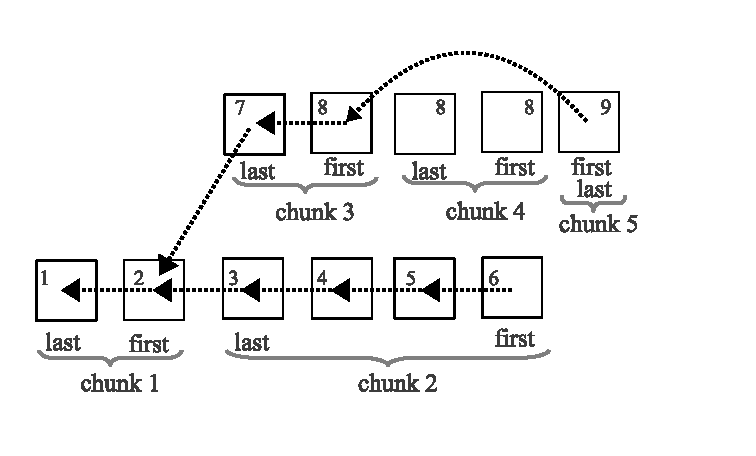
\includegraphics[width=0.6\linewidth]{pics/ChunkFull.eps}
	\caption{Чанки}
	\label{fig:chank1}
\end{figure}
Здесь изображено пять чанков. Друг с другом связаны через поле \texttt{first} следующие чанки: 5 и 4, 4 и 3, 3 и 1, 2 и 1. Чанк 4 являтся пустым. \texttt{first}  и \texttt{last} это первый и последний узлы чанков. Числа обозначают идентификатор узла. Отсюда видно что пустой чанк дублирует узел \texttt{first}. связанного слева с ним чанка.

Поясним смысл данной структуры. В отдельный чанк заносится информация о состоянии текущего шага логического вывода, поскольку информация разнородна, то для каждого конкретного случая тип {\tt T} конкретизируется. Связанные чанки образуют совокупность информации о шагах логического вывода.




%=================== ДЕРЕВО СОСТОЯНИЙ ВЫВОДА =======================
\subsection{Дерево состояний вывода}
Одним из основополагающих средств реализации поиска ЛВ в разработанной системе АДТ является \emph{дерево состояний вывода} (ДСВ), которое строится, в основном, при помощи структур данных, базирующихся на чанках. В структурах ДСВ, с одной стороны, хранится вся совокупность шагов вывода, по которой можно распознать какие действия были произведены на каком шаге, с другой стороны, ДСВ представляет текущую опровергаемую формулу. Основная задача ДСВ заключается в том, чтобы строго зафиксировать все события, произошедшие на каждом шаге логического вывода. Примером фиксируемого события является факт применения некоторой подстановки к в некоторой базовой подформуле к некоторому вопросу. Такая фиксация событий позволяет:
\begin{enumerate}
 \item Использовать больше информации о выполненных действиях, тем самым анализировать процесс ЛВ, а значит эффективно (в смысле большего разнообразия вариантов управления) внедрять эвристики в базовую стратегию поиска ЛВ.
 \item Производить поиск ЛВ с возвратом (backtracking) в процессе построения ЛВ.
 \item Реализовать стратегию разделения данных (data sharing) для случая расщепления базовых подформул после ответа на вопрос с дизъюнктивным ветвлением.
 \item Производить эффективное (в смысле удобства реализации системы АДТ и производительности) управление оперативной памятью.
\end{enumerate}

Идея использования ДСВ базируется на анализе свойств исчисления ПО--формул, проявляемых в процессе построения ЛВ. После каждого ответа на вопрос к первоначальной базовой подформуле добавляется пример консеквента этого вопроса: в базу добавляются соответствующие элементы узлов, непосредственно следующих за вопросом; к списку вопросов базы, в общем случае, добавляются новые вопросы; в случае дизъюнктивного ветвления база расщепляется. Таким образом, формула монотонно увеличивается, при этом сохраняя свою эвристическую структуру. ДСВ используется для обеспечения полного доступа к информации о текущем и прошлом состоянии поиска ЛВ формулы, а также для обеспечения возможности отката поиска ЛВ (backtracking) и подробного наблюдения (сбора статистики) за процессом поиска ЛВ.

Более детально, \emph{дерево состояний вывода} есть такое дерево, которое обладает следующими свойствами: корень дерева есть одна из базовых подформул исходной ПО--формулы; все остальные узлы есть добавляемые консеквенты с применёнными к ним подстановками--ответами с необходимым разыменованием переменных. Если приводить в пример определение правила вывода \ref{omega}, то корень дерева --- это база $B(\Phi)$, а узлы --- это $C_i(\Psi_i)\theta$. Таким образом если происходит расщепление базы то в соответствующем узле появляется ветвление. Теперь можно говорить, что каждая базовая подформула в формуле характеризуется соответствующим путём от листа ДСВ до её корня.

Как видно, каждый узел содержит достаточную информацию и для того, чтобы производить откат поиска, для этого достаточно просто удалять соответствующие узлы. Кроме того, такой подход реализует разделение данных (ссылок) на каждый консеквент, поскольку некоторые пути могут иметь общие подпути. Если какая-то база опровергнута, то можно удалить все узлы от соответствующего листа до ближайшей точки ветвления, поскольку оставшаяся часть пути всё ещё используется для представления другой базы. Количество листовых узлов ДСВ равно текущему количеству баз. Если дерево пусто, значит первоначальная база опровергнута. Так как изначальная формализация задачи в языке ПО--формул может содержать несколько базовых подформул, то для каждой из этих подформул строится своё ДСВ.

Для практических нужд разработки специализированных версий системы АДТ узел ДСВ позволяет сохранять некоторую системную информацию:
\begin{enumerate}
\item Множество атомов--фактов, добавленных к базе на данном шаге вывода (который характеризуется узлом ДСВ). Данное множество представляется как чанк. Отсюда каждый базовый конъюнкт на данном шаге вывода характеризуется объединением всех чанков от данного узла до корня, при этом чанки являются связанными.
\item Список ссылок на вопросы к базе, добавленные на данном шаге вывода. Как и в случае с базовым конъюнктов, вопросы представляются связанными чанками.
\item Для каждого вопроса хранится чанк соответствующих ответов на данном шаге вывода.
\item Номер последующего шага вывода и соответствующий ответ, если узел имеет потомков.
\item Чанк использованных ответов.
\end{enumerate}
Кроме того, узлы ДСВ содержат разнородную информацию, используемую как параметры к стратегиям поиска логического вывода.

При помощи чанков получается разграничивать данные, полученные на каждом шаге, т.е. всегда возможно определить какие данные на каком шаге выводы были добавлены, и какие события произошли. Под данными имеются ввиду: атомы--факты, вопросы, ответы и т.п. С другой стороны, на каждом шаге (в каждом узле) доступны все собранные до этого данные.

ДСВ для формулы из примера \ref{proofexample} представлено на рисунке рис.~\ref{fig:pst}. Корнем ДСВ является исходная ПО--формула $F_1$. Узел ``2'' является консеквентом вопроса $Q_1$, а именно $\exists\colon A(a)$, а путь от узла 2 до корня соответствует ПО--формуле $F_2$. Узлы 3 и 4 соответствуют консеквентам вопроса $Q_4$. Путь от узла 3 до корня и путь от узла 4 до корня соответствуют базовым подформулам ПО--формулы $F_3$. Например, формулы определённые путями 5---1 и 3---1 разделяют данные, которые представлены узлами 1---2. Если базовая подформула, которая представлена узлами пути 3---1 опровергнута, то можно удалить путь от узла 3 до ближайшего ветвления (в сторону корня), в данном случае удаляется только узел 3, поскольку узлы 2---1 всё ещё используются для представления других базовых подформул.
\begin{figure}[h]
	%\vspace{0.5cm}
	\centering
	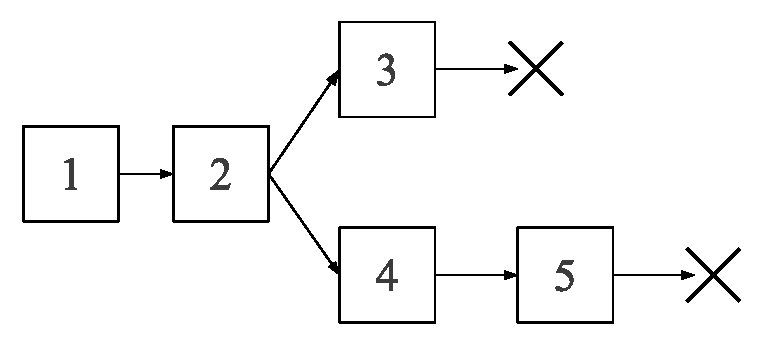
\includegraphics[width=0.4\linewidth]{pics/PST.eps}
	\caption{Дерево состояний вывода для формулы из примера \ref{proofexample}}
	\label{fig:pst}
\end{figure}
На следующем рисунке представлено ДСВ, как связанные чанки.
\begin{figure}[h]
	%\vspace{0.5cm}
	\centering
	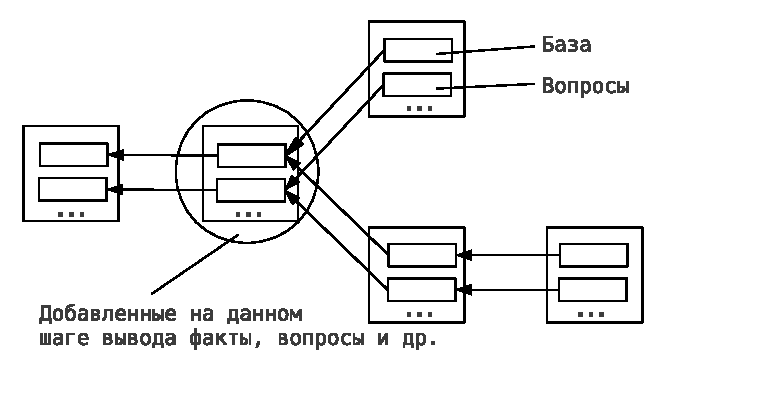
\includegraphics[width=0.6\linewidth]{pics/PST2.eps}
	\caption{ДСВ рис.~\ref{fig:pst}, представленное в виде чанковs}
	\label{fig:pst2}
\end{figure}

Специфика связывания чанков, характеризует ДСВ как дерево направленное от листьев к корню.
%\rem{С точки зрения реализации ДСВ растёт от листов к корню}{Не понял. Причем тут реализация? \app{М.б. это просто свойство структуры, как, например, в Linux директорий /var всегда растет.}}.

Для ДСВ реализована процедура редукции {\tt merge()}, преобразующая цепь узлов ДСВ в один узел. Это позволяет сократить используемую память, за счёт утраты подробной информации о шагах вывода, соответствующих цепочке узлов ДСВ.


%================================== СУПЕРВИЗОР =======================
\subsection{Супервизор}
Супервизор управляет процессом поиска ЛВ и собирает статистику о процессах со всего ДСВ. Он обеспечивает алгоритмы информацией об ограничениях ресурсов, используемых эвристиках и т.п. В супервизоре находится список всех текущих листовых вершин ДСВ. Большинство стратегий реализовано на уровне супервизора, поскольку, в общем случае, необходимо использовать информацию о всей совокупности предшествующего или последующего вывода.

Наличие супервизора обусловлено тем, что некоторые частные события в процессе логического вывода могут повлиять на ЛВ в целом. Супервизор осуществляет наблюдение за системой через контроллер доступа к ПО--формуле. Определены следующие операции: поиск выражений по логическому выводу; слияние нескольких узлов ДСВ в один; выделение процедур опровержения базовой подфомрулы в отдельный независимый поток, с последующим ожиданием результатов опровержения; назначение стратегий; прерывание вывода, для интерактивных шагов; доступ к глобальному кэшу, для использования кэшированных данных опровержения одной базовой подформулы в опровержении другой; удаление листов дерева; удаление ветвей от листа до ближайшего ветвления; общий сбор потребляемых ресурсов, проверка ограничений; исходная информация о ПО--формуле.

%============================================================================
%================================== РАЗДЕЛЕНИЕ ДАННЫХ =======================
\subsection{Разделение общей оперативной памяти структурами данных}
Логический вывод практически всегда связан с получением новой дополнительной информации, ростом объема используемой оперативной памяти. Например, в метод Резолюции выводятся (синтезируются) новые дизъюнкты до тех пор пока не получится пустой дизъюнкт, а в методе доказательства ПО--формул производится насыщение баз фактами до тех пор, пока все базы не станут содержать противоречие. Поскольку сложность формул может быть сколько угодно большой и даже минимальный вывод может иметь сколько угодно большую длину, имеет место проблема исчерпания имеющихся ресурсов вычислительной системы на хранение разрастающиеся структуры формулы. Опыт показывает \cite{TermIndexingBook}, что автоматический вывод довольно быстро занимает всю имеющуюся в распоряжении оперативную память, и далее процесс вывода требует регулярное удаление излишков. За излишки можно принять любые части формулы. Например, в некоторых системах, основанных на методе резолюций удаляются дизъюнкты, которые либо вообще не участвовали в выводе, либо не участвовали в нём определённое количество шагов, иногда удаётся определить что дизъюнкт больше не пригодится, либо предположить что не будет использоваться и возможно потерять полноту вывода. В случае ПО--формул, излишками являются устаревшие факты, фиктивные вопросы. Таким образом, проблема экономии оперативной памяти является основной проблемой, решаемой в диссертации, особенно с учётом увеличения сложности задач.

Для экономии памяти используются, во-первых, проектирование компактных структур данных; во-вторых, методы разделения общих участков оперативной памяти (data sharing). В случае логических языков и конкретно языка ПО--формул использование методик хранения информации с разделением общей памяти является продуктивным: экономия памяти позволяет строить как более глубокие, так и более широкие ЛВ. Исходя из некоторых общих особенностей представления языков первого порядка и представления ПО--формул, выделено и реализован ряд методик разделения данных.


\paragraph{Агрессивное разделение термов.} Данная методика заключается в том, что разделяются общие участки оперативной памяти среди термов. Например, в термах $A(g(a,f(x)),h(c))$ и $B(k,g(a,f(x)))$, подтермы $g(a,f(x))$ являются общими и представляют собой один и тот же участок в памяти. Данный подход позволяет экономить большие объемы оперативной памяти при ограниченных ресурсах, однако требует дополнительное процессорное время на вычисление общих подтермов. Каждый новый созданный терм (например, факт, добавляемый в базу) проверяется на наличие в нём подтермов, уже используемых где-либо, т.е. производится полный поиск подтермов по базе. Если подтерм найден, то для него переносится ссылка на уже существующий. Такой метод является общеупотребимым в системах АДТ, некоторые варианты реализации представлены в \cite{Ryazanov2003}.

\paragraph{Мягкое разделение термов} отличается от агрессивного подхода намного меньшим потреблением процессорных ресурсов, но и меньшей эффективностью с точки зрения объема экономии памяти, поскольку разделяет только часть общих подтермов. Исходя из определения \ref{ircond}, применение правила вывода $\omega$ корректно в случае выполнения условия $A\theta \subseteq B$, где $A$ и $B$, соответственно, конъюнкты вопроса и базы. Поскольку $B$ это уже существующее множество основных обобщенных термов, то для их хранения выделена соответствующая оперативная память. Подстановка $\theta$ же является отображением переменных вопроса $A$ в элементы эрбранова универсума. В дальнейшем при выполнении шага вывода $\theta$ применяется (апплицируется) ко всему консеквенту вопроса, и данный консеквент добавляется к формуле. Однако правая часть подстановки уже имеется в оперативной памяти в силу того, что основана она на термах из $B$. Исходя из этого, достаточно использовать ссылки на структуры и уже имеющуюся память, используемые для правых частей подстановки, в тех частях консеквента, где эта подстановка применяется.

Рассмтрим следующий фрагмент базовой ПО--формулы:

$$ \exists:A(f(e,g(t))) - \forall x:A(f(e,x)) - \exists:B(h(x),x) $$

В данном случае вопрос $\forall x:A(f(e,x))$ имеет ответ $\theta = \{x \rightarrow g(t)\}$. К базе фактов добавляется $B(h(x),x)\theta$, т.е. $B(h(g(t)),g(t))$. На рис.~\ref{fig:datasharing1} представлен пример, демонстрирующий данную ситуацию с точки зрения мягкого разделения памяти.
\begin{figure}[h]
	%\vspace{0.5cm}
	\centering
	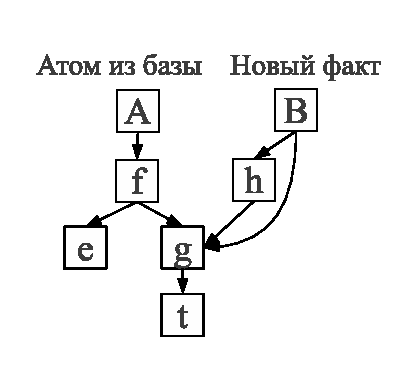
\includegraphics[width=0.3\linewidth]{pics/DataSharing1.eps}
	\caption{Мягкое разделение памяти термов}
	\label{fig:datasharing1}
\end{figure}

%------------Разделение по Черкашину------------
\paragraph{Разделение базовых подформул.} ПО--формулы, в которых производится ответ на вопрос с дизъюнктивным ветвлением, расщепляются на несколько новых базовых подформул. Количество новых базовых подформул совпадает с количеством непосредственных дизъюнктивных подформул в консеквенте вопроса. В простом варианте реализации ЛВ \cite{dissChe} такое расщепление требует копирования предыдущего состояния формулы несколько раз; такое копирование хотя и имеет линейную сложность \cite{Che2}, но всё равно естественно приводит к большим затратам памяти и процессорного времени, затрачиваемого для копирования. Разделение базовых подформул вполне реализуемо при помощи агрессивного разделения оперативной памяти термами. Однако, если формула предполагает достаточно сильное ветвление, сохраняется проблема наличия множества ссылок на разделяемые атомы баз, поскольку конъюнкт представляется как множество ссылок на атомы. Поскольку расщепление предполагает разделение общих частей баз, то имеет смысл разделять упомянутые выше ссылки. Данная стратегия реализуется за счёт средств ДСВ. Любая общая подветвь двух ветвей ДСВ является разделяемой. Рассмотрим небольшой пример. Пусть имеется следующая базовая подформула:
$$\exists: A(a) - \forall x: A(x) - \left\{
\begin{array}{lcl}
 \exists \colon B(x) & - & \forall y: B(y) - \exists\colon\boldsymbol{False}\\
 \exists \colon C(x) & - & \forall y: C(y) - \exists\colon\boldsymbol{False}
\end{array}
\right. $$
Обозначим первый и второй вопросы через $Q_1$ и $Q_2$ соответственно. ДСВ для вывода данной формулы представлено на рис.~\ref{fig:datahsaring2}.
\begin{figure}[h]
	%\vspace{0.5cm}
	\centering
	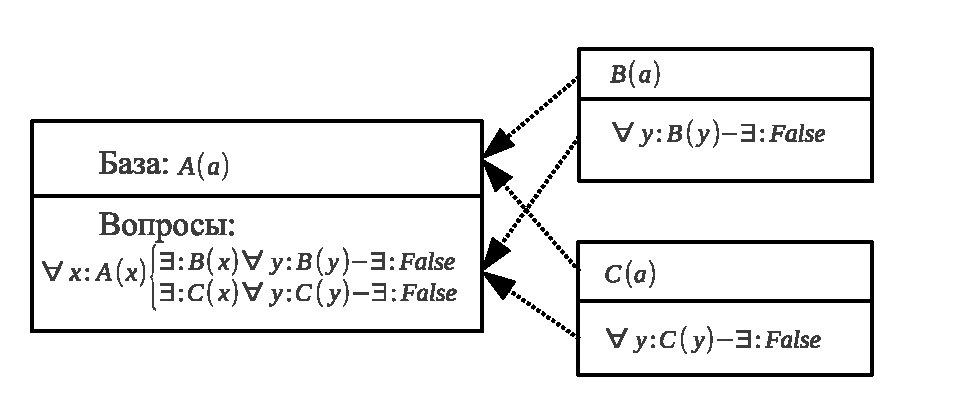
\includegraphics[width=0.7\linewidth]{pics/DataSharing2.eps}
	\caption{Пример ДСВ вывода подформулы}
	\label{fig:datasharing2}
\end{figure}

\paragraph{Разделение переменных и неопределенных эрбрановских элементов.} Данная методика предназначена для высокопроизводительного применения подстановки ко всей подформуле, т.к. все одноименные переменные в формуле представляют собой один участок в оперативной памяти. О неопределенных эрбрановских элементах сказано ниже. Все одноименные переменные на протяжении любого основного пути формулы \cite{dissChe} являются указателем на один и тот же участок в памяти. В отличие от агрессивного разделения данный подход учитывает роль переменных в процессе поиска ответных подстановок. В процессе применения подстановки переменная не заменяется на терм, а лишь указывает на этот терм, что позволяет экономить время на замену переменной термом в поддереве: достаточно одной операции присвоения над одной переменной, чтобы установить замену всех таких переменных в поддереве.


\paragraph{Удаление неиспользуемых фактов.} Ниже, показано что стандартная стратегия поиска ответных подстановок основана на том, что для каждого атома из конъюнктов вопросов производится попытка мэтчинга с каждым атомов--фактом из базы. Поскольку, количество вопросов и длина конъюнктов конечны, то нетрудно определить для атома--факта из базы, мэтчится ли он хотя бы с одним атомом из вопросов. Если нет, то такой атом--факт можно удалить из базы, поскольку он вообще не используется в поиске ответных подстановок. Удаление ненужных фактов так же позволяет экономить память и время на переборе фактов.

\paragraph{Веса подформул.} Под весом терма или подформулы понимается количество узлов в дереве, представляющем терм или подформулу. Анализ веса позволяет сдерживать разрастание формулы, и, соответственно, обеспечить дополнительную экономию потребляемой памяти. Для этого из возможных ответов на вопрос приоритет отдаётся тому, который приводит к формуле наименьшего веса.

%\rem{...}{Что насчет управления комбинациями методик? Откат и вес? Как задавать эти комбинации? ли это уже реализация, наверное.}

\paragraph{Ограничение ресурсов} Стратегия ограниченных ресурсов реализована в большинстве современных систем АДТ, в том числе и в Вампире \cite{Ryazanov2003}. В данной системе АДТ подобная стратегия зависит от текущего ДСВ и описывается следующим образом. Ветка ДСВ растет до тех пор, пока не наступит ограничение объема оперативной памяти, разрешенной для использования, либо пока не исчерпается определенное время, либо пока не будет произведено определенное количество шагов вывода. Если наступил предел использования ресурсов, то осуществляется откат назад и выбор других ответов, т.е. используются другие варианты построения дерева.

%======================== INDEXING ===========================
\subsection{Индексирование данных}

Формализации некоторых задач могут быть довольно обширными, например задача \texttt{ALG214+4} из библиотеки TPTP в языке ПО--формул занимает порядка 10~Мб. Кроме того, даже если изначальная формула не столь велика, после некоторого количества шагов вывода, она может разрастись до достаточно большого размера. Стратегии разделения данных позволяют лишь отсрочить момент переполнения памяти, а так же вместить в имеющуюся память формулу как можно большего размера.

С другой стороны существуют ситуации, когда необходимо анализировать ПО--формулу на наличие определённых свойств. Такой анализ проводится как в рамках логического вывода, так и отдельно. Например, если для задачи заданна некоторая стратегия вывода, то для осуществления очередного шага вывода выбирается ответ, а значит база и вопрос, соответствующий этой стратегии, т.е. анализируется вся формула, и выбираются удовлетворяющие стратегии части формулы. Кроме того анализ формул часто требуется после вывода формулы, для сбора статистики и другой информации, позволяющей в дальнейшем разрабатывать новые стратегии, либо извлекать содержательную информацию из ЛВ.

Отсюда необходимо разработать методы, позволяющие в формуле производить эффективный поиск необходимых её элементов (термов, вопросов, ответов). Для решения данной проблемы обратимся к существующему опыту.

%индексирование термов
\paragraph{Индексирование термов}
Основной структурой, используемой для представления формул является обобщенный терм. Он используется для представления элементов конъюнктов, кванторных переменных, обеих частей подстановок. Поэтому актуальной задачей является эффективный поиск обобщенных термов в формуле по заданным критериям.

В информационных технологиях поиск данных часто разрешаются, например, с помощью методов индексирования данных, применяемых широко в реляционных базах данных БД \cite{Ulman}. В нашем случае основной объект индексирования --- это обобщенный терм, который является древовидной структурой, индексирование которой методами, используемыми в  реляционных БД, неэффективно \cite{TermIndexingBook}. Поэтому используются нижеописанные подходы.

Индексирование термов к настоящему времени хорошо исследовано, как в рамках определенных систем АДТ, так и абстрактно. В частности по данной теме существует ряд интересных работ, в том числе \cite{disctree, pathindex, TermIndexingBook, HARIndex }. Представленные в этих работах методы позволяют эффективно находить в базе термов такие термы, которые удовлетворяют определенным критериям: являются равными данному (query term), являются его примерами, обобщениями (generalization) и унификациями. Для разработанной системы АДN требовалось обобщение и классическая унификация, но дополнительно необходимы методы индексной поддержки НЭЭ--унификации: критерий наличия термов, включающих заданный подтерм; различные количественные критерии: вес, глубина, арность. С учетом перечисленных требований а также того факта, что как правило, в базе находятся основные термы, качестве основы методики индексирования выбрано индексирование путями \cite{pathindex,disctree}. Кратко опишем её суть, как она описана в \cite{disctree}.

Для каждого символа входящего в терм составляется список так называемых \emph{путей}. Путь --- это последовательность чередующихся символов и чисел, где число определяет позицию символа среди дочерних узлов \cite{disctree}. Например, атом $A(e,f(f(x,k),y),m)$ представляется в виде путей $A$, $A1e$, $A2f$, $A2f1f$, $A2f1f1x$, $A2f1f2k$, $A2f2y$, $A3m$. То есть каждому символу соответствует путь от корня до этого символа в древовидном представлении обобщенного терма. Подробнее на рис.~\ref{pathfig}. Каждый из этих путей содержит указатель на соответствующий терм, т.е. тот терм, для которого строился путь. Сами пути хранятся в отсортированном виде (в дереве).
\begin{figure}[h]
	%\vspace{0.5cm}
	\centering
	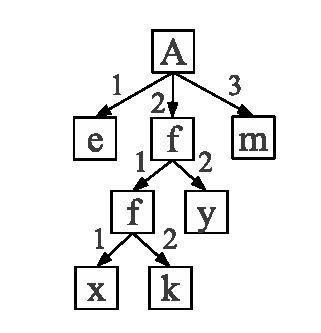
\includegraphics[width=0.2\linewidth]{pics/Path1.eps}
	\caption{Пример применения индексирования путями}
	\label{pathfig}
\end{figure}

Пример. Пусть дан атом $A(a,f(x,b))$ и множество атомов 
$$\{A(a,f(c,b)), A(a,f(b,e)),A(a,f(k,b)), A(b,f(e,b))\}$$. 
Любой атом, являющийся основным примером для заданного, содержит в своём списке путей следующие пути: $A1a$, $A2f2b$. Таким образом, для поиска основных примеров заданного атома необходимо найти пересечение множеств атомов, на которые указывают пути.  В частности путь $A1a$ указывает на множество 
$$\{A(a,f(c,b)), A(a,f(b,e)),A(a,f(k,b))\}$$, 
а путь $A2f2b$ на 
$$\{A(a,f(c,b)), A(a,f(k,b)), A(b,f(e,b))\}$$. 
Пересечение этих множеств есть множество $\{A(a,f(c,b)),A(a,f(k,b))\}$, это и есть множество примеров для атома $A(a,f(x,b))$.

Методы индексирования термов в настоящее время широко используются во многих известных системах АДТ. %: Vampire -улучшенное индексирование путями, Otter --- дискр.дерево и пути, E, EQP, SPASS --- дерево подстановок.

Кроме базы термов, в индексировании нуждаются множества вопросов и множества ответных подстановок. Поскольку количество вопросов не так велико как количество термов, то достаточно использовать возможности обычного словаря.

%индексирование других частей формулы
\paragraph{Индексирование других частей формулы}
Теперь опишем другие проблемы, решаемые при помощи методов индексирования данных. Предположим что пользователем задана некоторая стратегия для решения некоторого класса задач. Стратегия оперирует вопросами с определенными свойствами (т.е. с вопросом сопоставляется содержательная информация), которые присущи всему классу задач (т.е. все задачи объединяет наличие определенных вопросов). Для повышения производительности поиска ЛВ необходимо упростить в дальнейшем доступ к таким вопросам, чтобы каждый раз повторно не проверять все вопросы на наличие определенного свойства. Для этого достаточно сделать словарь (map) в котором каждому описанию вопроса соответствует указатель на данный вопрос. %\rem{В принципе, в стратегиях задавать опции при помощи номеров вопросов, но тогда теряется гибкость: пользователю необходимо ставить вопросы всегда на одно и тоже место. Данный вид индексирования (весьма простого) может выполняться как на этапе компиляции (тогда в компиляции прувера будет задействован не только стратегия но и сама задача), так и при первичном обращении к вопросу (тогда нет необходимости в компилировании самой задачи).}{О чем это?}


\paragraph{Индексирование ПО--формул} Доказательство крупных формул может производиться в несколько этапов, с сохранением промежуточных результатов на жесткие носители информации. Сам логический вывод формально является цепочкой формул. Для анализа описанных ситуаций необходимо проверять формулы на наличие некоторых свойств. Поскольку, ПО--формула как и обобщенный терм имеет древовидную структуру, то для её индексирования применимы описанные выше методы индексирования путями. Однако в данном случае индекирование путями требует доработки, поскольку, в случае термов путь однозначно задавался символами и номерами дочерниих узлов, то в случае ПО--формул номера дочерних узлов сохраняются, а вот символу может соответствовать любая формально описанная характеристика узла ПО--формулы (типового квантора). %[Буду дописывать данный параграф. Есть поле для размышлений. Можно на статью небольшую сделать. В книгах про индексирование подобные задачи описаны как нужные.]


%================================== ЛЕНИВАЯ КОНКРЕТИЗАЦИЯ =======================
\subsection{Неограниченные переменные}
\label{s:uhe}
Проблема неограниченных переменных описана выше. Кратко опишем её суть. Согласно определению \ref{ircond} правило вывода $\omega$ применимо в том случае если вопрос $\forall \bar{y}\colon A$ к базе $\exists \bar{x}\colon B$ имеет {\em ответ} $\theta$  такой что $\theta$ есть подстановка $\bar{y} \rightarrow H^{\infty}$ и $A\theta \subseteq B$. В случае если все перменные из $\bar{y}$ содержатся в конъюнкте $A$, то поиск соответствующих элементов из $H^{\infty}$ производится с помощью алгоритма поглощения. Если же среди $\bar{y}$ имеются переменные, которые не входят в $A$, то такие переменные называются \emph{неограниченными} и не используются в алгоритме поглощения. Однако для этих переменных необходимо найти подстановку, причём любой элемент эрбранова универсума является формально корректной подстановкой. Проблема в том, что в общем случае (при наличии функциональных символов) эрбранов универсум является бесконечным множеством, и какой именно элемент из него необходимо выбрать неизвестно.

Данная проблема не является тривиальной. Предложенною несколько подходов решения этой проблемы.

\subsubsection{Стратегия ленивых конкретизаицй}
Суть ленивой конкретизации заключается в следующем. В качестве подстановки для неограниченной переменной выбирается не конкретный элемент эрбранова универсума, а неопределенный эрбрановский элемент (НЭЭ), который, в дальнейшем, исходя из стратегии поиска необходимых термов для построения шага вывода, постепенно конкретизируется до основного терма, либо в некоторых ситуациях так и остается недоопределенным. В данном случае необходимые термы обеспечивают возможность ответа на вопрос: НЭЭ постепенно конкретизируется таким образом, что бы можно было на очередном шаге вывода построить новый ответ на какой--либо или заданный вопрос. Одновременно решается следующая задача: до какого терма конкретизировать НЭЭ, что бы появился ответ на вопрос? Отметим, что НЭЭ первоначально появляется как часть ответа в одном вопросе, а его конкретизация производится при поиске ответов на другие вопросы. Под <<постепенной конкретизацией>> понимается процедура ленивых вычислений: НЭЭ доопределяется на столько точно, на сколько этого достаточно для ответа на текущий вопрос, т.е. конкретизация может быть неполной (т.е. не конкретизирующая НЭЭ до основного терма), например НЭЭ $h$ конкретизируется до $f(h_1)$, где $h_1$ новый НЭЭ.

По своей природе НЭЭ схож с [неконкретизированной универсальной] переменной в том смысле, что он изменяем, т.е. потециально конкретизируем, однако все такие изменения должны быть направлены только на конкретизацию НЭЭ, т.е. НЭЭ заменяется только на некий терм (возможно тоже содержащий НЭЭ), либо на другой НЭЭ, но не на переменную. Однако, при замене переменной на НЭЭ, НЭЭ обладает всеми свойствами основного терма.

Рассмотрим пример приложения этой техники в процессе построения логического вывода для следующей формулы.
\begin{equation}
	\forall\colon\boldsymbol{True} - \exists\colon\boldsymbol{True} -
	\left\lbrace
	\begin{array}{l}
		\forall x\colon\boldsymbol{True} - \exists\colon A(x) \\
		\forall x\colon A(f(x)) - \exists\colon B(f(x)) \\
		\forall\colon B(f(a)) - \exists\colon \boldsymbol{False}
	\end{array}\right.
\end{equation}
На первом шаге вывода получен ответ $\{x \rightarrow h_1\}$ на первый вопрос, $x$ является неограниченной переменной, $h_1$ --- это неопределённый эрбрановский элемент (НЭЭ). После первого шага атом $A(h_1)$ добавляется в базу. На втором шаге вывода получен ответ $\{x \rightarrow h_2\}$ на второй вопрос, и $h_1$ конкретизируется до $f(h_2)$, после второго шага $B(f(h_2))$ добавляется в базу. Наконец, на третьем шаге получен тривиальный ответ на третий вопрос, и $h_2$ доопределяется до $a$.

В общем случае существуют особые ситуации. Рассмотрим следующий пример.
\begin{example}[]\label{example:uhe1}
$$\fictAquantor \; - \; \exists\colon M(e) \left\{
\begin{array}{lcl}
 \forall x,y\colon M(x) & - & \exists\colon S(y),M(f(x)),T(x) \\
 \forall x \colon T(x),S(e) & - & \exists\colon Q(x) \\
 \forall x \colon Q(x),S(f(e)) & - & \exists\colon\textbf{False}
\end{array}
\right.$$

Данная формула имеет вывод, например такой. Получаем ответ на первый вопрос подстановкой $\{ x\rightarrow e, y\rightarrow e \}$, в результате в базу попадают факты $S(e),M(f(e)),T(e)$; ответ на второй вопрос есть $\{ x \rightarrow e\}$, и в базу попадает $Q(e)$; полученных фактов в базе недостаточно для ответа на целевой вопрос, поэтому вновь отвечаем на первый вопрос, при этом возможно несколько вариантов ответа, но, что важно, переменную $y$ необходимо заменить на $f(e)$. Выберем, например, следующий ответ $\{x \rightarrow e, y \rightarrow f(e) \}$ и в базу попадет факт $S(f(e))$ после чего на целевой вопрос ответ получается. Заметим, что на первый вопрос необходимо обязательно выбирать те подстановки, которые содержат $y \rightarrow e$ и $y \rightarrow f(e)$, они необходимы для ответа на второй и третий вопросы, соответственно. Формула устроена таким образом что первый и второй вопросы всегда имеют новые ответы.

Теперь рассмотрим работу стратегии ленивой конкретизации. Ответ на первый вопрос будет следующего вида $\{ x\rightarrow e, y\rightarrow h_1 \}$, где $h_1$ --- НЭЭ, и в базу попадают следующие факты $S(h_1),M(f(e)),T(e)$. Ответ на второй вопрос --- $\{ x\rightarrow e, h_1\rightarrow e \}$, в котором $h_1$ доопределяется до $e$, и, соответственно, находящийся в базе факт $S(h_1)$ доопределяется до $S(e)$. С этого момента начинается выполнение, фактически, циклической операции, поскольку целевой вопрос не имеет ответа: вновь получаем ответ на первый вопрос, и вновь в базу попадает факт $S(h_1)$, который при ответе на второй вопрос вновь доопределится до $S(e)$ и т.д. Однако если пропустить ответ на второй вопрос, то при ответе на целевой, факт $S(h_1)$ доопределится до $S(f(e))$ и на этом вывод закончится.
\end{example}


В общем виде проблема заключается в том, что существуют ситуации, когда с формальной точки зрения НЭЭ конкретизируется корректно, но не там где это требуется, например раньше, чем это необходимо при ответе на другой вопрос. Либо НЭЭ может конкретизироваться там где это уже не требуется. Из подобных примеров видно, что ленивая конкретизация не всегда может использоваться на прямую. Необходимы дополнительные эвристические средства обеспечения логического вывода, учитывающие описанные только что проблемы.

%------------первый вариант
\paragraph{Ограничение количества конкретизаций}
Два НЭЭ будет называть \emph{подобными}, если они получены в результате выбора подстановки для одной и той же переменной. Такая ситуация имеет место если на один и тот же вопрос с неограниченными переменными произведено несколько ответов, и для неогарниченных переменных все разы в качестве подстановки выступает новый НЭЭ.

Ограничение одинаковых конкретизаций для подобных НЭЭ позволяет исключить ситуации, когда НЭЭ доопределяется там, где это уже не требуется, и, как следствие, появляется возможность конкретизировать его в другом месте. Для каждого НЭЭ хранится ссылка на переменную, для которой этот НЭЭ был выбран как подстановка. В вопросах каждой неограниченной переменной соответствует набор термов, до которых доопределялись НЭЭ соответствующие данной переменной. Таким образом, имеется возможность отслеживать сколько раз и до чего конкретизировался данный НЭЭ. Если лимит конкретизаций закончен, то процедура матчинга заканчивается неудачей. Выбор конкретного числа, ограничивающего количество конкретизаций, определяется либо пользователем, исходя из его знаний о задче, либо это число изначально устанавливается равным $1$, и, далее, это число увеличивается в случае неуспешности вывода за определенное количество шагов или времени.

Использование данного подхода позволяет решить пример \ref{example:uhe1} за 5 шагов, если установить единице лимит конкретизаций для переменнй $y$ из первого вопроса. Посольку $h_1$ не будет конкретизироваться до $e$ второй раз, во втором вопросе.

%--------------------ещё вариант
\paragraph{Сохранение выражений, содержащих НЭЭ}
Представим другой вариант управления стратегией ленивых конкретизаций. Описанный выше вариант конкретизаций НЭЭ, в том числе используемый в примере \ref{example:uhe1}, не сохраняет исходное выражение, содержащийся в котором НЭЭ конкретизируется. Отсюда возникает проблема потери информации. Например, если в примере \ref{example:uhe1} в базу попадает атом $S(h_1)$, то при необходимости конкретизации $h_1$, конкретизация производится не в самом атоме, а пораждается новый атом, такой, как если бы был конкретизирован исходный, т.е. в случае рассматриваемого примера, к базе добавляется атом $S(e)$, при этом атом $S(h_1)$ сохраняется. НЭЭ $h_1$ сохранён, а значит может использоваться в других вопросах.

Содержательно такой подход означает следующее. Можно считать, что для вопроса с открытыми переменными применяется вся совокупность возможных ответов, т.е. с использованием всех элементов эрбрановского универсума. Понятно, что это технически нереализуемо из--за бесконечности эрбановского универсума, поэтому и используется техника ленивых вычислений. В идеале предполагается, что за один раз используются все возможные ответы на вопрос, но на самом деле используются только необходимые ответы. Например, если в некоторой формуле содержится вопрос $\forall x: True  - \exists A(x)$, и $H^{\infty}= \{a, f(a), f(f(a)), ...\}$, то использование всех возможных ответов разом приводит к попаданию в базу элементов $\{A(a), A(f(a)), A(f(f(a))), ...\}$, которых бесконечно много. Вместо этого множеству ставится в соответствие элемент $A(h)$, где $h$ --- НЭЭ, и в дальнейшем этот элемент пораждает необходимые элементы множества $H^{\infty}$.

В данном случае можно заметить сходство со стратегией ленивых конкретизаций, без каких--либо ограничений. Преимущество подхода с сохранением выражений, содержащих НЭЭ, заключается в том, что выражение, содержащее НЭЭ всегда сохраняется, т.е. не может быть утрачено за счёт применения каких-либо подстановок.

Рассмотрим отдельно два случая. Если конкретизируемый НЭЭ содержится в подформуле-вопросе, и если конкретизируемый НЭЭ первоначально появился после ответа на вопрос с дизъюнктивным ветвлением.

В случае с дизъюнктивынм ветвлением, вся совокупность оветов на вопрос означает не просто появление бесконечного конъюнкта, а бесконечно множества конъюнктов, поскольку база ещё и расщепляется. Т.е. конкретизация НЭЭ приводит не просто к пораждению нового атома в конъюнкте, а к очередному расщеплению формулы, в той точке логического вывода, в которой впервые появился доопределяемый НЭЭ. Данную точку легко отследить благодаря структуре ДСВ, в которой сохраняются все события произошедшие на каждом шаге вывода. Однако ветвление целесообразно проводить не в этой точке, а во всех листах дерева, корнящегося из этой тчоки. Поскольку вставка втевления в середину вывода потребует копирования для каждого нового узла той части вывода которая была уже прозведенаа.  На рис.~\ref{lazy21} схематично показано некоторое ДСВ.
\begin{figure}[h]
	%\vspace{0.5cm}
	\centering
	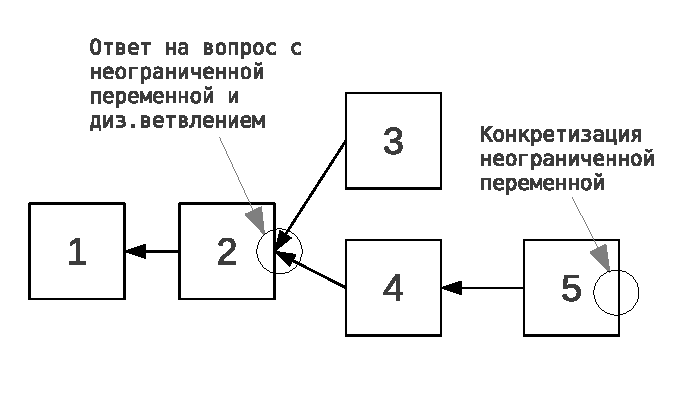
\includegraphics[width=0.5\linewidth]{pics/Lazy21.eps}
	\caption{Структура ДСВ до конкретизации}
	\label{lazy21}
\end{figure}
После конкретизации НЭЭ, получаем структуру ДСВ, изображенное на рис.~\ref{lazy22}.

\begin{figure}[h]
	%\vspace{0.5cm}
	\centering
	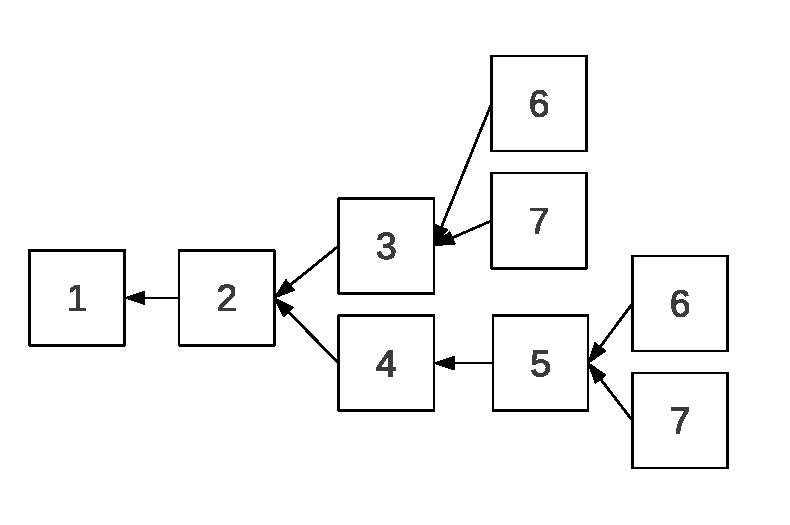
\includegraphics[width=0.5\linewidth]{pics/Lazy22.eps}
	\caption{Структура ДСВ после конкретизации}
	\label{lazy22}
\end{figure}

В случае подформулы--вопроса, содержащего НЭЭ, конкретизация НЭЭ требует пораждения новой подформулы--вопроса, отличающейся от исходной только в точке содержания НЭЭ. Возможно появление множества вопросов, усложняющее в целом структуру формулы и её вывод. Под усложнением структуры, в данном случае, понимается именно наращивание количества вопросов. Абсолютный размер формулы (в байтах) меняется незначительно, поскольку используются стратегии экономии памяти. Новую подформулу--вопрос целесообразно вставлять в той точке вывода (перед этим узлом), где первоначально добавился вопрос с НЭЭ. Предположим что на рис.~\ref{lazy21} вопрос с НЭЭ впервые появляется в узле 2. Тогда если конкретизация НЭЭ потребуется в любом из последующих узлов, дерево преобразуется в вид, как на рис.~\ref{lazy23}. При этом новый узел 6 содержит только новый пораждённый вопрос.
\begin{figure}[h]
	%\vspace{0.5cm}
	\centering
	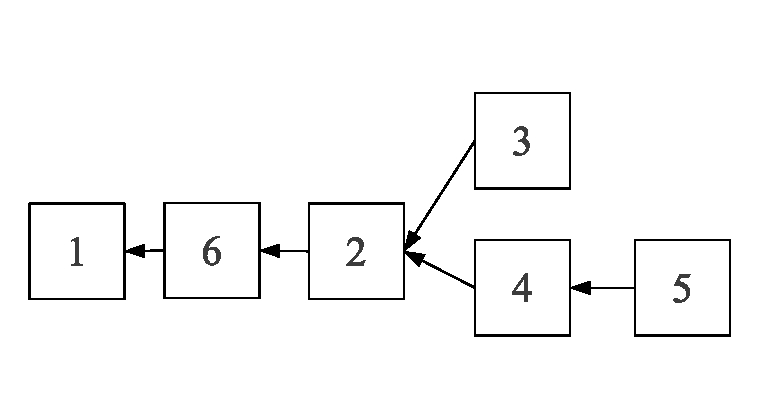
\includegraphics[width=0.5\linewidth]{pics/Lazy23.eps}
	\caption{..}
	\label{lazy23}
\end{figure}

%---------------второй вариант
\paragraph{Ручное управление}
Одним из вариантов решения проблемы является использование языка описания стратегий, с помощью которого можно, например, указать, что на второй вопрос необходимо ответить лишь один раз, либо использовать на первый вопрос сразу несколько подстановок содержащих $y\rightarrow h_1$ и $y\rightarrow h_2$. Это приведет к попаданию в базу двух фактов $S(h_1)$ и $S(h_2)$, один, из которых будет использоваться для второго вопроса, а другой для целевого. Такой вариант вполне приемлем, и может использоваться для решения задач. Такой подход в настоящее время пока не обеспечивает принципиальную выводимость, но для отдельных классов задач он уместен. %\rem{Но что делать, если дополнительные знания о задаче не позволяют сформулировать правильную стратегию? Необходимо предоставить хотя бы принципиальную возможность вывода, что пока необеспеченно.}{Удалить м.б.}

%-------------
Отметим, что стратегии, основанные на использовании НЭЭ, создают некоторые проблемы совместимости с другими стратегиями. Во-первых, при использовании этой стратегии нарушается независимость базовых подформул, поскольку один и тот же НЭЭ может быть в разных подформулах: доопределение общего НЭЭ в одной подформуле автоматически приводит к доопределению его в другой подформуле. Этот факт, в частности, делает зависимыми процессы поиска ЛВ в базовых подформулах на параллельных вычислительных архитектурах. %Он также противоречит некоторым эвристическим уточнениям алгоритмов и стратегий, например, {...}{Пошел простой пример стратегии.}. Во-вторых, ...

\subsubsection{Cтратегия фильтрации эрбрановского универсума}
Другим вариантом (помимо стратегии ленивых конкретизаций) решения проблемы неограниченных переменных, является \emph{стратегия фильтрации эрбрановского универсума}. Данная стратегия позволяет избавиться от изложенных в начале главы проблем, но несколько расширяет пространство возможных ответов. Суть данной стратегии заключается в следующем. В консеквентах, атомы, которые содержат неограниченные переменные вопросов, должны унифицироваться с одноимёнными атомами из всех других частей всей базовой подформулы, в противном случае атом попавший в базу не будет удовлетворять условию применения правила вывода (\ref{ircond}), поскольку никода не выполнится процедура матчинга при поиске ответов. Будем использовать данное свойство в стратегии. В качестве ответа для неограниченных переменных используются такие термы, что атом полученный подстановкой переменных на эти термы будет основным примером найденной унификации. Такой подход позволяет заранее сузить пространство эрбрановского универсума, фильтруя заведомо бесполезные ответы.

Для ясности рассмотрим пример. Пусть имеется следующие вопросы ПО--формулы.
$$Q_1 = \forall x,y: - \exists: A(f(x,g(y)))$$
и
$$Q_2 = \forall x:A(f(e,x)) - \exists: False$$

В данном случае в консеквенте вопроса $Q_1$ содержится атом $A(f(x,g(y)))$. Одноимённый атом, это атом вопроса $Q_2$, а именно $A(f(e,x))$. Унификация двух данных атомов есть $A(f(e,g(y)))$. Основной пример данного атома есть любой, атом полученный из исзодного заменой переменной $y$ на любой элемент $H^{\infty}$. Тогда ответ для вопроса $Q_1 = \{x \rightarrow e, y \rightarrow t\}$, где $t$ любой элемент $H^{\infty}$, например $e$. В базу попадёт факт $A(f(e,g(e)))$ и ответ на целевой вопрос будет $\{x \rightarrow e\}$.

Такой подход имеет сходство со стратегий ленивых конкретизаций, в которой конкретизация НЭЭ, по сути, означает сужение эрбранова универсума, до множества основных примеров конкретизации. В данном же случае ограничения на ЭУ накладываются сразу, исходя из потенциальных вопросов. В случае стратегии ленивой конкретизации, конкретизация как раз производится при поиске ответов на эти потенциальные вопросы.

Данная стратегия позволяет всегда работать с полностью конкретизированной формулой, т.е. формулой не содержащей НЭЭ.

%=============================================================================================
%======================================================================
%================================== k,m-ограничение =======================
\subsection{Стратегия $k,m$--ограничения}
Данная стратегия формулируется следующим образом. Некоторый ответ применяется, если за последующие $k$ шагов произойдет заданное событие по меньшей мере $m$ раз. Пользуясь терминологией ДСВ, это означает, что для данного узла дерева применяется ответ в случае, если построенное в результате дальнейшего вывода поддерево, коренящееся с этого узла, не превысит глубину $k$, и до этого момента произойдет $m$ раз заданное событие. Предложено три специальных случая данной стратегии.

\paragraph{$k,m$--опровержение.} Заданный ответ выбирается в случае, если за последующие $k$ шагов ЛВ будет опровергнуто как минимум $m$ баз. Подобная стратегия, а именно $k$--опровержение, первоначально предложена А.К.~Жерловым в \cite{ICDS2000} и реализована в системе КВАНТ/1 Черкашина Е.А. \cite{dissChe}, где показана её состоятельность. В данной системе эта стратегия расширена вторым параметром $m$. Она позволяет сдерживать разрастание пространства поиска вывода, т.е., сдерживает излишнее ветвление ДСВ, что в некоторых случаях приводит к многократному усложнению вывода.

Отметим, что выбор параметров $k$ и $m$, заранее не определён, и пользователю необходимо знать следующие нюансы. Во-первых, параметр $k$ означает что будут проверены все возможные ответы на глубине $k$ шагов, т.е. произведен полный перебор, что в свою очередь может затратить большие ресурсы процессорного времени и памяти. Параметр $m$ дополнительно усиливает, условие выбора исходного ответа. Поэтому, если заранее нельзя предположить какие выбрать эти параметры, то по умолчанию они устанавливаются $k=1$ и $m=p$, где $p$ количество непосредсветнных дочерних дизъюнктивных узлов вопроса, и в случае неудачи ЛВ, параметр $k$ постепенно увеличивается, а $m$ уменьшается.

\paragraph{$k,m$--конкретизация.} Иная спецификация стратегии $k,m$--ограничения, формулируется так. Ответ на вопрос принимается, если за последующие $k$ шагов будет доопределено $m$ НЭЭ. Эта стратегия также направлена на то, чтобы ограничить сложность представляемой формулы. С недоопределенным НЭЭ ассоциируется много дополнительной информации и условий, описанных в разделе \ref{s:uhe} о неограниченных переменных, что на уровне реализации влияет негативно. Поэтому чем больше и быстрее НЭЭ будут доопределены, тем лучше.

\paragraph{Особенности реализации стратегии $k,m$--ограничения}
Основной для реализации данной стратегии являются описанные выше ДСВ и супервизор. Параметры $k,m$ и, собственно, условие задаются в супервизоре и привязываются к определённом узлу ДСВ. Супервизор проверяет все условия на каждом шаге ЛВ. И в положительном случае (когда условие выполнено) производится возврат поиска (backtracking) назад, т.е. производится последовательное удаление узлов дерева в обратном порядке (от листа в направлении корня). Перед удалением каждого узла производится разконкретизация НЭЭ, полученных в этих узлах и возврат использованных вопросов в стадию активных (т.е. возможных для применения).

%================================== КЕШИРОВАНИЕ =======================
\subsection{Кэширование результатов}
Учитывая множественность возможных ответов, возвратов поиска в выводе, большой глубины вывода, большого количества атомов в базе и т.д. целесообразно кешировать некоторые результаты чтобы не производить снова повторяющиеся вычисления.

Добавление уже имеющихся в базе атомов не допускается. Поэтому процедура поиска ответов работает всегда с новыми атомами, и производит всегда новые вычисления. Тем не менее полученные ответы в итоге могут совпадать. Все примененные ответы сохраняются, причем хранятся они как и база в чанках, расположенных по всему пути от листа до узла. Это позволяет делать корректные возвраты поиска с учетом сохранения информации о примененных ответах.

Некоторые подзадачи поиска ответных подстановок являются часто повторяемыми операциями. Поэтому для таких подзадач вводится кэширование результатов. Например, совмещение нескольких ответных подстановок.

%\rem{...}{Тут можно было б таки описать, как кэш используется. Что строиться - понятно. А как используется и где, когда, не понятно. Мартьянов, похоже, как то так делает в своих задачах составления расписания.}

%-----------PARALLEL STRATEGY---------------------------
\subsection{Параллельные стратегии}

Повышение производительности достигается при помощи вышеописанных интенсивных методов, ориентированных на оптимизацию использования вычислительных ресурсов, а также при помощи экстенсивных методов, базирующихся на вовлечении в процесс дополнительных вычислительных ресурсов. В частности, это становится актуальным ввиду широкого распространения многоядерных вычислительных систем общего назначения, в частности, рабочих станций.

Одним из популярных экстенсивных методов повышения производительности является разработка версий программ АДТ для кластерных архитектур в параллельном режиме исполнения ветвей подпрограмм. Рассмотрим методики и стратегии построения параллельных реализаций алгоритмов поиска ЛВ в исчислениях ПО--формул. Предложены следующие стратегии для построения параллельных схем алгоритмов поиска логического вывода.

\paragraph{Первая стратегия: опровержение баз}

В случае, если вопрос имеет дизъюнктивное ветвление, то после ответа на этот вопрос, формула расщепляется и трансформируется в формулу с б\'{о}льшим количеством баз, т.е. в общем случае, количество базовых подформул увеличивается с каждым шагом вывода. С другой стороны, исходная формализация задачи в языке ПО--формул, опять же в общем случае, содержит более одной базовой подформулы. Для того, что бы показать, что исходная формула противоречива, необходимо опровергнуть каждую из баз. Специфика исчисления ПО--формул позволяет производить логический вывод и опровержение этих баз независимо друг от друга. Данное свойство называется естественным ИЛИ--параллелизмом, который следует из того что в базах находятся лишь основные термы. Поэтому процедура опровержения каждой базы может выполняться в отдельном вычислительном процессе или на отдельном вычислительном устройстве.

Таким образом, первая стратегия, реализуемая в виде параллельной схемы алгоритмов, формулируется следующим образом: каждая базовая подформула, содержащая только основные термы в базе, опровергается независимо от других базовых подформул, а значит для этот процесс выделяется в отдельный параллельный независимый от других процесс, синхронизируемый с другими процессами только  на этапах его создания в момент расщепления формулы и завершения в момент установления выводимости/невыводимости. Во время жизни этого процесса к нему может поступать асинхронный сигнал завершения от супервизора, обозначающий, что выполнение процесса далее не имеет смысла, например, формула является неопровержимой, что было доказано в какой-либо другой ветка поиска доказательства, или пользователь остановил выполнение программы. Для программной реализации алгоритмов данной стратегии созданы подпрограммы жесткого копирования и маршаллинга/демаршаллинга, что бы полностью скопировать базовую подформулу и обрабатывать её в отдельном процессе независимо, т.е. не разделяя оперативную память.

%\rem{...}{Думаю этот раздел немного покажет тебе на сколько подробно можно и надо писать.}

\paragraph{Вторая стратегия: поиск ответов на вопросы}
Для применения каждого шага логического вывода, необходимо выполнять, в общем случае, поиск ответных подстановок для заданного вопроса. Поиск ответных подстановок не изменяет структуру формулы, и не использует общих изменяемых данных, это значит, что процессы поиска ответа на каждый вопрос независимы, а значит параллельны. Отметим, что поиск ответных подстановок для одного вопроса является намного менее трудоёмкой задачей, чем опровержение базовой подформулы, но тем не менее если конъюнкт вопроса содержит достаточно много атомов, то поиск всех ответных подстановок усложняется, за счёт увеличения пространства --- в общем случае декартова произведения множеств подстановок для каждого атома из конъюнкта.

%\rem{...}{М.б. тут тоже рассказать в общих чертах о варианте реализации, например, что это не будет отдельный процесс или узел, а будет поток (нить)}


\paragraph{Третья стратегия: поиск подстановок для атомов конъюнкта вопроса}
Теперь рассмотрим процедуру поиска подстановок для отдельно взятого вопроса. Как было сказано во введении, подстановка $\theta$ является ответом, если выполняется условие $A\theta \subseteq B$, где $B$ --- конъюнкт вопроса, $A$ --- конъюнкт базы. Для сохранения полноты необходимо хотя бы потенциально иметь в распоряжении все возможные ответы, из которых выбирается подстановка для данного шага. Ниже описана структура хранилища ответов. Наполнение каждого чанка хранилища подстановками производится параллельно, поскольку чанки независимы.

\paragraph{Свойства стратегий}

Анализ, описанных выше стратегий, показывает, что они обладают свойством вложенности. Т.е., для того, что бы опровергнуть одну базовую подформулу (первая стратегия) необходимо найти ответы на вопросы (вторая стратегия). В свою очередь для поиска ответа, необходимо найти подстановки для каждого атома из конъюнкта вопроса (третья стратегия).

Исходя из этого, данные стратегии можно разместить по степени эффективности (иерархия стратегий). Не трудно видеть, что время, затрачиваемое на опровержение базы, как минимум, не меньше, чем время, затрачиваемое на поиск ответных подстановок, а на практике, как правило, оказывается намного больше, так как для опровержения базы необходимо неоднократно ответить на некоторые вопросы. Аналогичные выводы делаются по отношению к другим стратегиям.

Кроме того, можно выделить единое для всех стратегий свойство –-- свойство однородности. Т.е. стратегии имеют единую структуру. А именно, все они, по сути, сводятся к применению некоторой операции (опровержение базы, поиск ответов и т.д.) для каждого элемента некоторого множества (базы, вопросы и т.д.).

Одной из рекомендаций при реализации описанных алгоритмов на кластерных вычислительных системах является правильное распределение задач между вычислительными узлами кластера, в зависимости от скорости коммуникации между ними. Например, программная реализация первой стратегии должна процесс привязывать к вычислительному узлу. Привязка процесса к вычислеительному узлу, в случае второй стратегии, возможна с увеличением конъюнкта вопроса и увеличением множеств подстановок, соответствующих каждому атому вопроса. В противном случае, этого не стоит делать, как и  при реализации третьей стратегии, так как коммуникационные затраты, вполне вероятно, перекроют полезное время вычислений, и тем самым лишь ухудшат результат.

%Отметим что данная стратегия в общем случае конфликтует со стратегией отсроченного присваивания (поскольку СОП может нарушать независимость баз и вопросов). \rem{...}{А это не надо было где-то раньше сказать. Например в разд. ``первая стратегия''?}

\paragraph{Тестирование}
Важным свойством параллельных схем алгоритмов является их масштабируемость, т.е. степень повышения эффективности с увеличением количества вычислительных элементов (ВЭ). Поэтому основной характеристикой является не конкретное время исполнения программ, а соотношение времени исполнения программы в параллельном режиме на заданном количестве ВЭ к времени исполнения этой же программы на одном ВЭ при различном количестве ВЭ.

Эксперименты проводились на задачах, формализация которых в языке ПО--формул обладает необходимыми свойствами для испытания параллельных стратегий, а именно: дизъюнктивное ветвление, большое количество вопросов, крупные конъюнкты вопроса. Результаты находятся в соответствии с представленной иерархией стратегий. На рис. \ref{fig:parallel} представлены результаты данного тестирования.
\begin{figure}[h]
	%\vspace{0.5cm}
	\centering
	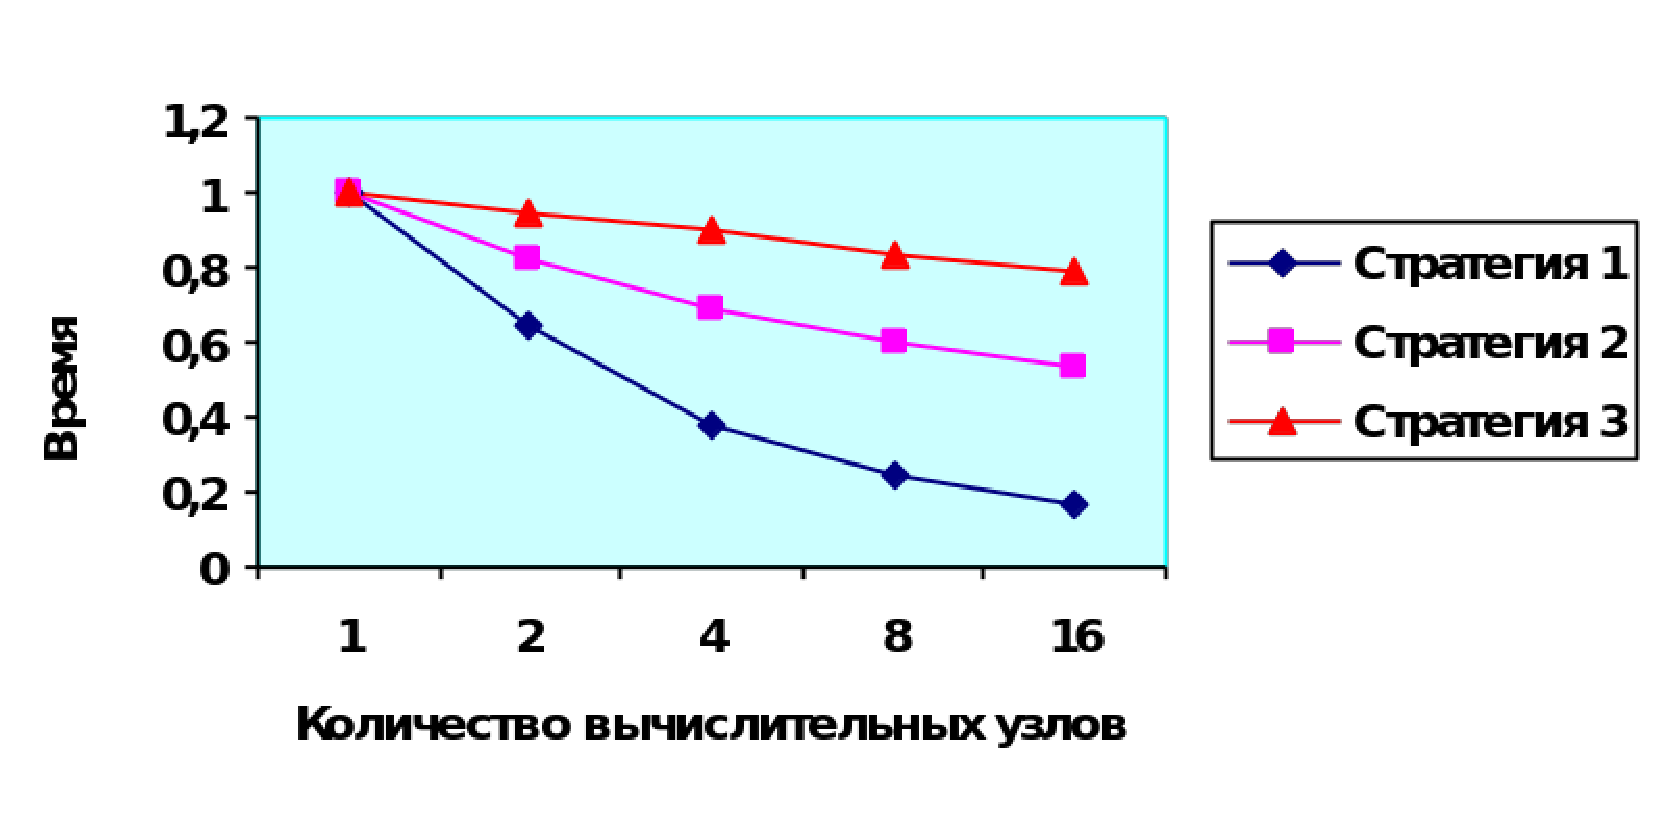
\includegraphics[width=0.7\linewidth]{pics/Parallel.eps}
	\caption{Результаты тестирования параллельной реализации алгоритмов АДТ, согласно представленной стратегии}
	\label{fig:parallel}
\end{figure}

Наибольшую эффективность, как и следовало ожидать, показала первая стратегия, естественно при наличии дизъюнктивного ветвления в исходной формуле. Под эффективностью понимается уменьшение затрачиваемого времени с увеличением количества вычислительных узлов.


%============================= РАВЕНСТВА =========================
\subsection{Равенства}
Для обработки предиката равенства, как правило, крайне неэффективно напрямую использовать аксиомы равенства (рефлексивность, симметричность, транзитивность, подстановочность) без специальной адаптации алгоритмов АДТ. Например, если формула содержит лишь один бинарный функциональный символ $f$ и один бинарный атомарный символ $A$, то в языке ПО--формул аксиомы равенства для такой формулы будут представлены следующим образом.
$$\left\lbrace
\begin{array}{l}
\forall x\colon\boldsymbol{True} - \exists\colon x = x \\
\forall x_1,y_1,x_2,_y2\colon x_1 = y_1, x_2 = y_2 - \exists\colon f(x_1,y_1) = f(x_2, y_2) \\
\forall x_1,y_1,x_2,_y2\colon x_1 = y_1, x_2 = y_2, A(x_1,y_1) - \exists\colon A(x_2,y_2)
\end{array}\right.
$$
Как видно, для каждого функционального и атомарного символа из формулы ставится в соответствие подформула--вопрос --- аксиома равенства. Явное использование таких аксиом, во-первых, усложняет структуру формулы (появляются лишние вопросы), во-вторых, значительно увеличивает число шагов вывода, в-третьих, генерирует много (потенциально бесконечно) фактов в базе, возможно не участвующих в выводе, а также мешающих выводу. Отметим, что данная проблема не так ужасна как в МР, поскольку в МР, в общем случае,  порождаются дополнительные дизъюнкты, а это соответствует порождению дополнительных вопросов в ПО--формуле. В исчислении ПО--формул порождаются лишь атомы-факты, за которыми проще наблюдать, в силу их более простой структуры, чем подформулы-вопросы (или дизъюнкты)

Очевидно, что вопросы--аксиомы равенства предназначены для того что бы выводить те и только те атомы--факты, которые эквивалентны по модулю $E(B)$, другим атомам-фактам из базы $B$. В данном случае $E(B)$ это все равенства из базы $B$.

Для того чтобы не использовать на прямую аксиомы равенства, предлагается генерировать эквивалентные по модулю $E(B)$ атомы--факты с помощью систем переписывания термов (СПТ) \cite{Nipkow}.

Для построения СПТ по равенствам в базе, используется известный алгоритм Кнута--Бендикса (Knuth--Bendix completion procedure) \cite{KBAlg}. Алгоритм Кнута--Бендикса, получая на входе множество атомов--равенств и редуцирующий порядок над термами \cite{Nipkow} строит эквивалентную конвергентную СПТ. Конвергентность СПТ означает что для каждого терма существует и только одна конечная форма (нормальная форма), которая может быть получена за конечное число переписываний. Под порядком над термами имеется ввиду отношение строгого частичного порядка над множеством термов. В нашем случае используется лексикографический порядок.

С помощью правил переписывания генерируются новые атомы--факты, эквивалентные, уже имеющимся в базе. В сочетании со стратегией удаления неиспользуемых фактов (стратегия экономии памяти), очевидно, что базу не будут добавляться ненужные сгенерированные факты.

Отметим, что такой подход не нарушает основных особенностей исчисления ПО--формул. Правило вывода сохраняется, остаётся единственным и унарным. Ответные подстановки по прежнему зависят лишь от базы, и не зависят от других вопросов. Базы попрежнему остаются независимы и содержат основные термы. Структура формулы не изменяется.

%В классическом подходе, в соответствии с определением ~\ref{ircond}, подстановка $\theta$ является ответом на вопрос, тогда и только тогда, когда $A \theta \subseteq B$ где $A$ --- конъюнкт вопроса, а $B$ --- конъюнкт базы. Поиск ответов есть задача поглощения, для решения которой, как правило, используется алгоритм матчинга \rem{, об этом уже писалось выше}{Это нужно?}. В случае ПО--формул используется основной матчинг, а в случае НЭЭ используется полуосновной матчинг. \rem{...}{Надо прокомментировать где-то ранее эти матчинги, или даже строго определить.}


%Для решения проблемы основного матчинга без явного использования аксиом равенства поставлена задача реализации основного матчинга с равенствами, которая формулируется следующим образом [microsoft]:
%\begin{quote}
%Для данного множества равенств $E(B)$, основного терма $t$ и терма $p$, который может содержать переменные, необходимо найти множество подстановок $\theta$, по модулю $E(B)$, такие что $E(B)\models t = p\theta$. Через $E(B)$ мы обозначим множество всех равенств в данной базе $B$. Две подстановки эквивалентны если их правые части попарно конгруэнты по модулю $E(B)$.
%\end{quote}

%С точки зрения реализации

%Для поиска таких ответов использован аппарат теории систем переписывания термов \cite{Nipkow}.

%=====================================================================
%==========================ХРАНИЛИЩЕ ОТВЕТОВ==========================
\subsection{Хранилище подстановок}
Хранилище подстановок предназначено для эффективной организации доступа алгоритмов к ответными подстановками и возможности организации механихзма бэктрэкинга, для приведения возможных ответов в предыдущие состояния (состояния на предыдущих шагах вывода).

Каждому атому конъюнкта вопроса соответствует чанк возможных подстановок, обеспечивающих матчинг этого атома с атомами из базы. Использование чанков связано с тем что необходимо точно определять на каком шаге какие подстановки были найдены. Для поиска ответа на вопрос, необходимо использовать алгоритм композиции подстановок для каждого атома из вопроса. На рис.~\ref{fig:anbase} представлена схема хранения подстановок для каждого атома.
\begin{figure}[h]
	%\vspace{0.5cm}
	\centering
	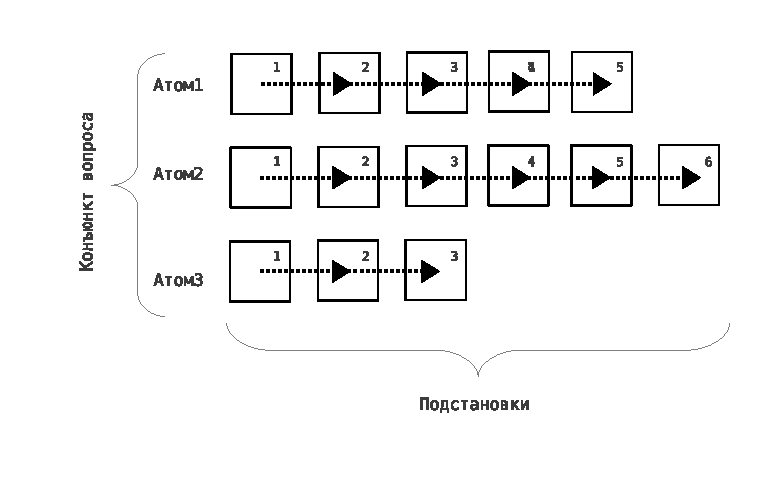
\includegraphics[width=0.6\linewidth]{pics/AnBase.eps}
	\caption{Подстановки}
	\label{fig:anbase}
\end{figure}

Из этой структуры выделяется ответ на вопрос, конъюнкту которого соответствует хранилище. Для этого комбинируются подстановки из каждого чанка по одной. При этом подстановки должны быть совместимы. Две подстановки совместимы если их левые части равны, а правые унифицируемы. Например, если есть подстановки $\{x \rightarrow a\}$ и $\{x \rightarrow b\}$, где $b$ есть константа, то эти подстановки несовместимы, поскольку $a$ и $b$ неунифицируемы. А подстановки $\{x \rightarrow f(a)\}$ и $\{x \rightarrow f(h)\}$, где $h$ есть НЭЭ, совместимы, поскольку $f(a)$ и $f(h)$ унифицируемы с подстановкой $\{h \rightarrow a\}$. Результатом комбинации будет объединение всех совместимых и унифицирующих подстановок.

Перебор подстановок из чанков производится последовательно, это позволяет сохранить полноту.

%=================================================================================
%==================================СТАНДАРТНАЯ СТРАТЕГИЯ==========================
%=================================================================================
%\subsection{Стандартная стратегия \app{поиска логического вывода}}
%Главное свойство стандартной стратегии \app{поиска логического вывода} заключается в её полноте. Для полноты вывода необходимо организовать полный последовательный перебор всевозможных ответов на все вопросы. Для этого используются возможности дерева состояний вывода и хранилища ответов. \rem{...}{Надо, я так понял, стратегию описать здесь подробно. Или зачем тогда раздел?}


%%% Local Variables:
%%% mode: latex
%%% TeX-master: "dis"
%%% End:

% Программная система
%\chapter{Реализация алгоритмов программной системы}\label{part:three}

Глава \ref{part:three} посвящена реализации структур данных, стратегий, алгоритмов и программных средств разработки системы автоматического доказательства первопорядковых теорем в исчислениях позитивно--образованных формул. В качестве исходной информации для реализации выступают результаты, полученные в предыдущей главе диссертации. Реализация включает средства автоматизации анализа количественных и структурных характеристик процесса поиска ЛВ, а также средств управления ЛВ. В результате реализации создана программная система АДТ и среда поддержки разработки систем АДТ, ориентированные как на практические задачи, так и на абстрактные задачи, традиционно, считающиеся математическими.



%=====================================================================
%---------------------------------АРХИТЕКТУРА-----------------------
%=====================================================================
\section{Архитектура системы}
На рис.~\ref{fig:design1} изображена архитектура программной системы. В основе подхода к проектированию архитектуры системы использовалась методика проектирования последовательной конкретизации (``сверху--вниз'') \cite{yodan}. Архитектура представляет собой набор взаимодействующих друг с другом функциональных блоков (подсистем).
\begin{figure}[h]
	%\vspace{0.5cm}
	\centering
	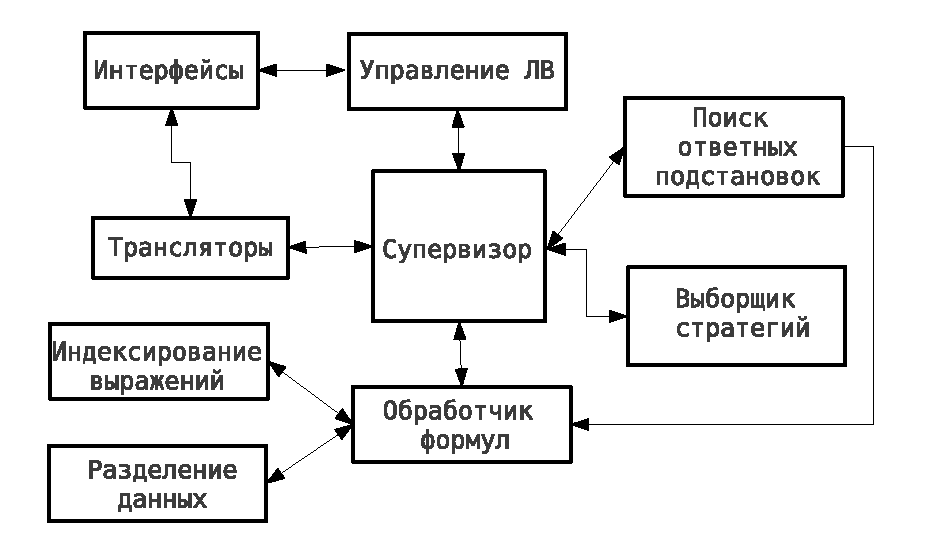
\includegraphics[width=0.7\linewidth]{pics/Design1.eps}
	\caption{Архитектура системы}
	\label{fig:design1}
\end{figure}

Программная система АДТ состоит из следующих функциональных блоков:
\begin{description}
  \item{Супервизор} --- подсистема глобального управления процессом поиска ЛВ и реализации выбранных стратегий. Особенности некоторых стратегий требуют анализа и модификации имеющихся данных в оперативной памяти во всех подпрограммах поиска ЛВ. Для поддержки реализации стратегий реализована подсистема, которая анализирует характеристики процессов исполнения подпрограммами ЛВ и полученных в них результатов. По запросам из подпрограмм Супервизор выдает необходимую статистическую информацию, на основе которой принимается то или иное решение в алгоритме реализации стратегии. Данная подсистема реализована как отдельный поток исполнения, ожидающий сигналов.
  \item{Выборщик стратегий} --- подсистема выбора стратегий, в которой на основе структурной и статистической информации о ПО--формуле и ЛВ выбирается та или иная подпрограмма, реализующая соответствующую стратегию поиска ЛВ.
  \item{Поиск ответных подстановок} --- подсистема поиска подстановок и ответных подстановок.
  \item{Обработчик формул} --- подсистема анализа и преобразований ПО--формул, в которой реализовано преобразование исходной ПО--формулы во внутреннее представление, снабжение этого представления вспомогательной информацией, используемой в ходе поиска ЛВ.
  \item{Транслятор} --- подсистема трансляции формул исчисления предикатов и КНФ, представленных в нескольких форматах, в ПО--представление.
  \item{Интерфейсы} --- подсистема интерфейсов к системе АДТ, включая интерфейсы прикладного программирования и интерфейс пользователя системы.
  \end{description}

Разработанная система устанавливает не только тот факт, что формула является теоремой, но и в некоторых случаях позволяет распознавать некоторые противоречия. В частности, распознаются случаи, когда хотя бы одна из ветвей ДСВ не может больше изменяться по причинам, не связанным с ограничением ресурсов и при условии, что не использовалось ограничений, влияющих на полноту вывода. Такой случай характеризуется отсутствием допустимых вопросов и ответов на вопросы, т.е. ветвь принципиально неопровержима.

В следующих разделах опишем подробно каждую подсистему.


%=====================================================================
%================================== СУПЕРВИЗОР =======================
%=====================================================================
\section{Супервизор}
Супервизор управляет процессом поиска ЛВ и собирает статистику о процессах со всего ДСВ. Он обеспечивает алгоритмы информацией об ограничениях ресурсов, используемых эвристиках и т.п. Супервизор ссылается на все текущие листовые вершины ДСВ. Большинство стратегий реализовано на уровне супервизора, поскольку, в общем случае, необходимо использовать информацию о всей совокупности предшествующего или последующего вывода.

Наличие супервизора обусловлено тем, что некоторые частные события в процессе ЛВ могут повлиять на ЛВ в целом. Супервизор осуществляет наблюдение за поведением системы через Обработчик ПО-формул. Определены следующие операции: поиск выражений по ЛВ; слияние нескольких узлов ДСВ в один; выделение процедур опровержения базовой подформулы в отдельный независимый поток, с последующим ожиданием результатов опровержения; назначение стратегий; прерывание вывода и переход в режим интерактивного построения шагов; доступ к глобальному кэшу для использования кэшированных данных опровержения одной базовой подформулы в опровержении другой; удаление листов дерева; удаление ветвей от листа до ближайшего ветвления; общий сбор потребляемых ресурсов, проверка ограничений; предоставление исходной информации о ПО--формуле.



%=====================================================================
%========================ВЫБОРЩИК СТРАТЕГИЙ===========================
%=====================================================================
\section{Выборщик стратегий}
Данная подсистема отвечает за выбор необходимых стратегий, улучшающих эффективность поиска ЛВ. Выбор осуществляется автоматически, исходя из структурных характеристик опровергаемой ПО--формулы. Ряд стратегий выбирается в самом начале поиска ЛВ и используется на протяжении всего процесса поиска ЛВ. Другие стратегии выбираются подпрограммами обработки текущего вопроса.

Ниже приведена таблица условий применения стратегий.

\begin{center}
Таблица 3.1. -- Выбор стратегий
\end{center}

\begin{longtable}[H]{|p{0.3\linewidth}|p{0.3\linewidth}|p{0.3\linewidth}|}
\hline
\textbf{Название стратегии} & \textbf{Уровень применения} & \textbf{Условие применения}\\
\hline
$k_1,m_1$--опровержение & подформула-вопрос & есть дизъюнктивное ветвление \\
\hline
$k_2,m_2$--конкретизация & подформула-вопрос & есть неограниченные переменные \\
\hline
$k$--неопровержимость & подформула-вопрос & есть дизъюнктивное ветвление \\
\hline
Ленивая конкретизация (ограничение 1) & подформула-вопрос & пустой конъюнкт \\
\hline
\end{longtable}

\newpage
\begin{center}
Продолжение таблицы 3.1. 
\end{center}

\begin{longtable}[H]{|p{0.3\linewidth}|p{0.3\linewidth}|p{0.3\linewidth}|}
\hline
\textbf{Название стратегии} & \textbf{Уровень применения} & \textbf{Условие применения}\\
\hline
Ленивая конкретизация (ограничение 2) & подформула-вопрос & нет дизъюнктивного ветвления \\
\hline
Фильтрация эрбранова универсума & базовая подформула & Используется 1-ая параллельная стратегия или количество видов функциональных символов < $f_{max}$ \\
\hline
Параллельная стратегия (вариант 1: по базам) & вся формула & есть вопрос с дизъюнктивным ветвлением \\
\hline
Параллельная стратегия (вариант 2: по вопросам) & базовая подформула & количество вопросов > $q_{min}$ \\
\hline
Параллельная стратегия (вариант 3: по атомам вопроса) & подформула-вопрос, базовый конъюнкт & размер конъюнкта вопроса > $qc_{min}$ и размер базового конъюнкта > $bc_{min}$  \\
\hline
Переписывание термов в базе & вся формула & наличие предиката равенства \\
\hline
Индексирование & вся формула & безусловное применение \\
\hline
\end{longtable}


\newpage
\begin{center}
Продолжение таблицы 3.1. 
\end{center}

\begin{longtable}[H]{|p{0.3\linewidth}|p{0.3\linewidth}|p{0.3\linewidth}|}
\hline
\textbf{Название стратегии} & \textbf{Уровень применения} & \textbf{Условие применения}\\
\hline
Мягкое разделение термов & вся формула & безусловное применение \\
\hline
Разделение данных по базам & вся формула & безуловно используется как часть ДСВ, но фактически проявляет себя в подформулах-вопросах с дизъюнктивным ветвлением \\
\hline
Агрессивное разделение термов & вся формула & любые ограничения памяти, установленные пользователем \\
\hline
Удаление неиспользуемых фактов & вся формула & достигнут предел памяти \\
\hline
Веса подформул & вся формула & любые ограничения памяти, установленные пользователем \\
\hline
%\end{tabular}
\end{longtable}


Параметрам $k, k_1, m_1, k_2, m_2$ изначально присваивается значение $1$. Дальнейшее их увеличение зависит от успешности применения стратегии с исходными параметрами. Если стратегия $k,m$--ограничения для всех ответов дала отрицательный ответ, то параметр $k$ увеличивается. Когда достигнуто максимальное значение $k$, то изменяться параметр $m$. Максимальное значение $k$ конфигурируется перед запуском программы.

Параметры $f_{max}, q_{min}, qc_{min}, bc_{min}$ конфигурируется перед началом работы программы. Подробнее о файле конфигурации ниже.

%=============================================
\paragraph{Файл конфигурации стратегий.}
Стратегии и критерии задаются при помощи конфигурационного файла. Формат файла представляет собой список двоек вида \texttt{<key>=<value>}, где ключ \texttt{<key>} --- идентификатор стратегии, критерия и т.п., а \texttt{<value>} --- значение данного ключа. Данные ассоциации помещаются в супервизор и, далее, используются в процессе поиска ЛВ.

Кроме того, в данном файле задаются следующие ограничения: максимальная глубина терма; максимальное количество вопросов; максимальная глубина вывода; максимальное количество базовых подформул; максимальный объём потребляемой памяти; ограничение по времени.




%=====================================================================
%==========================ПОИСК ОТВЕТОВ==========================
%=====================================================================
\section{Поиск ответных подстановок}
В данном разделе опишем механизмы поиска и хранения ответных подстановок.


%====================================================
\subsection{Хранилище подстановок}
Хранилище подстановок предназначено для эффективной организации доступа алгоритмов к ответными подстановками и возможности организации механизма бэктрэкинга. Хранилище позволяет осуществлять переходы в пространстве состояния поиска ЛВ, например, производить откат процесса на предыдущие состояния.

Каждому атому конъюнкта вопроса соответствует чанк возможных подстановок, обеспечивающих мэтчинг этого атома с атомами из базы. Использование чанков связано с тем, что необходимо точно определять на каком шаге и какие подстановки были найдены. Для поиска ответа на вопрос, необходимо использовать алгоритм композиции подстановок для каждого атома из вопроса. На рис.~\ref{fig:anbase} представлена схема хранения подстановок для каждого атома.
\begin{figure}[h]
  %\vspace{0.5cm}
  \centering
  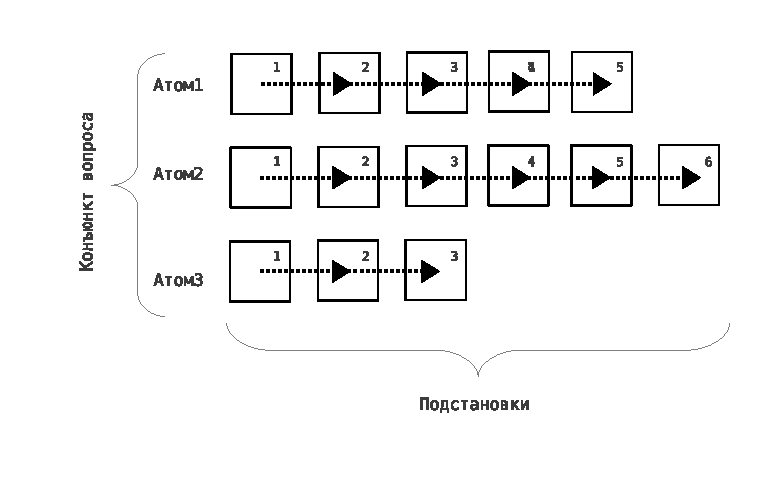
\includegraphics[width=0.7\linewidth]{pics/AnBase.eps}
  \caption{Подстановки}
  \label{fig:anbase}
\end{figure}

Из этой структуры выделяется ответ на вопрос, конъюнкту которого соответствует свое хранилище. Для этого комбинируются подстановки из каждого чанка по одной. При этом подстановки должны быть совместимы. Две подстановки совместимы если их левые части равны, а правые унифицируемы. Например, если есть подстановки $\{x \rightarrow a\}$ и $\{x \rightarrow b\}$, где $b$ есть константа, то эти подстановки несовместимы, поскольку $a$ и $b$ неунифицируемы. А подстановки $\{x \rightarrow f(a)\}$ и $\{x \rightarrow f(h)\}$, где $h$ есть НЭЭ, совместимы, поскольку $f(a)$ и $f(h)$ унифицируемы с подстановкой $\{h \rightarrow a\}$. Результатом комбинации будет объединение всех совместимых и унифицирующих подстановок.

Перебор подстановок из чанков производится последовательно, это позволяет сохранить полноту.


%=======================================================================================
\subsection{Композиция подстановок}

Хранилище подстановок содержит подстановки для отдельных атомов конъюнкта вопроса. Для того, чтобы получить ответ на вопрос, необходимо произвести композицию подстановок, соответствующих всем атомам конъюнкта вопроса. Хотя и существуют известные классические алгоритмы композиции подстановок, опишем такой, который учитывает особенности НЭЭ, а также особенности реализации структуры обобщенного терма, а именно использование аргумента как места для подстановки.

Пусть дан список подстановок $QList$, дана пустая подстановка $Answer$, называемая результирующей. Алгоритм последовательно просматривает все подстановки $q \in QList$ и производит композицию $Answer$ и $q$. В случае удачи алгоритм переходит к следующему элементу $QList$, иначе алгоритм возвращает NULL, т.е. заканчивается неудачей.

Теперь опишем алгоритм композиции $Answer$ и $q$. Связью (binding) будем называть часть подстановки вида $\{x \rightarrow t\}$, т.е. одинарная подстановка для одной универсальной переменной или НЭЭ. Соответственно, подстановка есть список связей. %Упомянуть во второй главе.
Для каждой связи $b_i \in q$ произвести композицию $b_i$ и $Answer$, в случае неудачи какого--либо шага, возвращается \texttt{NULL}.

Теперь опишем алгоритм композицию связи $b$ и подстановки $Answer$. Для каждого элемента $a \in Answer$ проводим композицию $b$ и $a$. В случае удачи, проводим композицию результата и $Answer$, берём следующий элемент $Answer$.

%Что такое ``Применить'' связь. Подстановка. Определить во второй главе.
Рассмотрим вариант композиции двух связей $b$ и $a$. Применить связь $b$. Если связь $a$ стала рекурсивной (аналог проверки вхождения терма, occur check), т.е. правая часть содержит левую, то алгоритм заканчивается неудачей, связь $b$  сбрасывается. Иначе, если левые части $b$ и $a$ различаются, то возвратить результат объединения $b$ и $a$. Иначе, если левые части совпадают, то, если хотя бы одна из подстановок уже применена и правые части совпадают алгоритм возвращает любую из подстановок, иначе алгоритм терпит неудачу; если обе подстановки не применены, то выполняем алгоритм унификации правых частей. Если он закончился успехом, то возвратить подстановку и унификацию, иначе возвратить \texttt{NULL}.



%====================================================================================
\subsection{Мэтчинг с НЭЭ}

В системе реализован вариант классического алгоритма мэтчинга (mat\-ching), адаптированный для случая содержания в термах НЭЭ. Пусть дано два терма $q$ и $b$, соответственно из базы и конъюнкта вопроса. Отметим, что поскольку $b$ --- это терм из базы, то он не содержит универсальных переменных. Задается пустая подстановка $a$, которая будет дополняться позже.
\begin{enumerate}
\item Если $q$ --- это константа. Тогда, если $b$ тоже константа, проверить их корневые символы, если совпадают, то вернуть $a$, иначе вернуть \texttt{NULL}. Если $b$ --- это НЭЭ, то применить подстановку $\{b \rightarrow q\}$ и добавить её к $a$, возвратить $a$. Во всех остальных случаях возвратить \texttt{NULL}.

\item Если $q$ --- это экзистенциальная переменная. Если $b==q$, то возвратить $a$. Если $b$ --- это НЭЭ, то применить подстановку $\{b \rightarrow q\}$ и добавить её к $a$, возвратить $a$. Во всех остальных случаях возвратить \texttt{NULL}.

\item Если $q$ --- это универсальная переменная, то применить подстановку $\{q \rightarrow b\}$ и добавить её к $a$, возвратить $a$.

\item Если $q$ --- это НЭЭ. Если $b$ тоже НЭЭ, то если $b==q$ вернуть $a$, иначе вывод разделяется на две части, в первом случае алгоритм возвращает \texttt{NULL}, во втором случае применить подстановку $\{q \rightarrow b\}$ и добавить её к $a$, возвратить $a$. Если $b$ --- тегирован как \texttt{FUNCTION}, то, если $q$ является подтермом $b$ возвратить \texttt{NULL}. Во всех остальных случаях применить подстановку $\{q \rightarrow b\}$ и добавить её к $a$, возвратить $a$.

\item Если $q$ тегирован как \texttt{FUNCTION}. Если $b$ тоже тегирован как \texttt{FUNCTION}, то если корневые символы $q$ и $b$ не совпадают, то возвратить NULL. Если совпадают, то это одноименные функции, одинаковой арности. Последовательно применить алгоритм мэтчинга для всех попарно соответствующих термов. Если применение алгоритма возвращает не \texttt{NULL}, то результат применить (как подстановку) и добавить к $a$. Если получен \texttt{NULL}, то отменить $a$ и вернуть \texttt{NULL}. Если $b$ --- это НЭЭ, то применить подстановку $\{b \rightarrow q_s(h_1,...,h_n)\}$ и применить алгоритм мэтчинга ко всем парам $(h_i, q_i)$, где $q_s$ --- это корневой символ $s$, $n$ --- арность $q$, $h_i$ --- новые НЭЭ, $i = \bar{1,n}$. Полученные результаты применить и добавить к  $a$, возвратить $a$.
\end{enumerate}





%=====================================================================
%======================ПРЕОБРАЗОВАНИЯ ВЫРАЖЕНИЙ========================
%=====================================================================
\section{Обработчик формул}

\subsection{Копирование подформул}
В системе реализовано два типа копирования подформул \emph{мягкий} (soft copy) и \emph{жесткий} (hard copy). Жесткий тип копирования предназначен для корректного копирования консеквентов и перемещения их к базе. Такое перемещение должно разорвать связь между переменными и их конкретизациями, для того чтобы освободить переменную для дальнейшего использования в других шагах вывода, но при этом, чтобы в базу попали именно те термы, до которых данная переменная конкретизирована. Кроме того, такой тип копирования нужен для параллельных стратегий, чтобы переместить формулу в полностью независимый процесс.

Второй тип копирования, мягкий, предназначен для корректной обработки НЭЭ с учетом бэктрэкинга. Поскольку при откатах поиска необходимо восстанавливать информацию о том какой НЭЭ был конкретизирован каким термом. Копирование НЭЭ осуществляется копированием его ссылки с сохранением его конкретизации. Потом такой НЭЭ в базе идентифицируется как конкретизированный и работа ведется с привязанным термом.

Копирование подформул в процессе шага вывода, требует, во--первых, разыменования всех экзистенциальных переменных, и всех неконкретизированных универсальных переменных. Поскольку структура копируемых подформул является древовидной, то для копирования применяется рекурсивный алгоритм, начинающий свою работу с корня дерева. Опишем подробно схему алгоритма копирования.

В начале работы алгоритма задан пустой словарь переменных, которые необходимо разыменовывать и соответствующих им разыменованных переменных. В скопированном узле (типового квантора) для его кванторных переменных создаётся новый список переменных той же длины что и исходный и того же типа (\texttt{EVARIABLE} или \texttt{AVARIABLE}), данный список есть копия исходного списка переменных, а в словарь заносятся соответствия между исходными переменными и новыми. Далее копирование конъюнкта требует создание нового конъюнкта такой же длины что и исходный, в который последовательно заносятся копии содержащихся в нём термов. Копирование термов производится рекурсивно. Создаётся новый корневой узел, в котором символ определяется следующим образом:  если исходный символ это неконкретизированная переменная (либо \texttt{EVARIABLE}), и она уже входит в словарь, то её копией будет соответствующее ей значение в словаре. Это делается для того, чтобы одинаково разыменовать одинаковые переменные. Если переменная конкретизирована, то копируется значение функции {\tt get\_value()}. Отметим, что не существует ситуации, когда встречается неконкретизированная переменная, которой нет в словаре, поскольку используются только замкнутые формулы, а в словарь последовательно добавляются все переменные управляемые кванторами; если исходный символ имеет тип \texttt{CONSTANT}, \texttt{FUNCTION}, \texttt{ATOM} или \texttt{EVARIABLE}, не содержащаяся в словаре, то новый символ есть ссылка на исходный. Далее для терма копируются все его аргументы. После того как копирование конъюнкта завершено, копируется системная информация о типовом кванторе. Далее процедуре копирования дочерних узлов передаётся текущий словарь, который реализован с помощью чанков, для того, чтобы более глубокие (по сравнению с исходным) узлы могли разделять информацию о словаре переменных.
%этап использования алг. (В каком контексте используется.)


%=====================================
\subsection{Шаг вывода} Когда выбран вопрос и ответ на этот вопрос, производится трансформация формулы, согласно определению \ref{omega}.
Данная трансформация состоит из следующих шагов:
\begin{enumerate}
\item Применить ответную подстановку (\texttt{answer.apply()}).
\item Произвести копирование подформул-консеквентов заданного вопроса с применением мягкого и жесткого копирования. Для каждого консеквента создаётся отдельный узел ДСВ.
\item Сбросить ответную подстановку.
\item Связывание полученных подформул--копий с имеющейся базовой подформулой. То есть, связывание полученных узлов ДСВ с соответствующим листом ДСВ.
\item Возврат результатов полученных в ходе данной операции.
\end{enumerate}


%==========================================
\subsection{Предобработка структуры формул}
Предобработка структуры ПО--формул используется для упрощения формулы, которое, вероятно, влечет уменьшение сложности поиска ЛВ. Упрощение формулы достигается удалением очевидно ненужных фиктивных кванторов, слиянием нескольких вопросов в один, уменьшение глубины формулы и т.п. При этом происходит уменьшение сложности, в основном, сокращается длина вывода и пространство поиска переборных алгоритмов.




%=====================================================================
%===========================ВЫБОР ВОПРОСА ============================
%=====================================================================
\section{Выбор вопроса} % Потенциально 2 главы материал
Алгоритм выбора вопроса базируется на нескольких стратегиях. Первая стратегия, стратегия по умолчанию, задает вопросам приоритет в соответствии со следующим правилом. Сначала просматривается список целевых вопросов. Затем, если для них не получен ответ, то просматриваются простые вопросы, не являющиеся глубокими и не содержащие дизъюнктивное ветвление. Далее просматриваются глубокие вопросы, затем все остальные, в т.ч. с дизъюнктивным ветвлением.

Вторая стратегия реализует выбор вопроса по критерию. Критерий выбора --- это некоторая количественная или структурная характеристика вопроса (подформулы). Примерами критериев выступают размер конъюнкта, наличие определенных термов в конъюнкте, частота удачного использования вопроса в ЛВ (рейтинг вопроса). Вопросам сопоставляется значение заданного критерия как приоритет использования вопроса. Вопросы, которым не присвоены значения критериев считаются низкоприоритетными. % Описать алгоритм выбора вопроса при заданных приоритетах.

%Третья стратегия --- это ручной выбор очередного вопроса пользователем.




%=====================================================================
%=====================МЕНЕДЖЕР ПАМЯТИ====================================
%=====================================================================
\section{Менеджер памяти}

Как было сказано выше, одна из методик экономии памяти --- это проектирование компактных структур данных. Под компактностью, в частности, понимается оптимизированное использование оперативной памяти. Выделение (allocation) оперативной памяти для структур (records) фиксированного размера реализовано на основе стандартного подхода, аналогичного \cite{gmemory} с формированием однонаправленного списка свободных структур (freelist). Массив структур отводится при помощи менеджера памяти операционной системы, и, затем, преобразуется в однонаправленный список свободных структур. Новые структуры выделяются из этого однонаправленного списка. При освобождении структура возвращается обратно в этот список для повторного использования. При исчерпании структур в списке и наличии свободной оперативной памяти выделяются новые массивы.

В системе АДТ для каждой разновидности структур (records) выделяется собственный массив, а также ведется собственный однонаправленный список свободных структур. Сборка мусора синхронизирована со сборщиком мусора используемой системы программирования D.


%=====================================================================
%================================== КЕШИРОВАНИЕ =======================
%=====================================================================
\section{Кэширование результатов}
Учитывая множественность возможных ответов, возвратов поиска в выводе, большой глубины вывода, большого количества атомов в базе и т.д. целесообразно кешировать некоторые результаты чтобы не производить снова повторяющиеся вычисления.

Добавление уже имеющихся в базе атомов не допускается. Поэтому процедура поиска ответов работает всегда с новыми атомами, и производит всегда новые вычисления. Тем не менее полученные ответы в итоге могут совпадать. Все примененные ответы сохраняются, причем хранятся они как и база в чанках, расположенных по всему пути от листа до узла. Это позволяет делать корректные возвраты поиска с учетом сохранения информации о примененных ответах.

Некоторые подзадачи поиска ответных подстановок являются часто повторяемыми операциями. Поэтому для таких подзадач вводится кэширование результатов. Например, совмещение нескольких ответных подстановок.



%=====================================================================
%======================ТРАНСЛЯТОР================================
%=====================================================================
\section{Транслятор из TPTP в ПО--формулы}
Одной из задач разработки системы АДТ является оценка производительности системы на стандартном наборе тестовых задач TPTP (Thousands of Problems for Theorem Provers) \cite{tptp}. Этот набор задач включает в себя широкий спектр проблем, найденных авторами архива в литературе, а также задач, найденных пользователями и переданными в архив по e--mail.

Задачи в архиве представлены в виде текстовых файлов, состоящих из двух основных частей: комментария, где представлена метаинформация о задаче, и собственно определения на специальном языке. Язык позволяет представлять формулы по отдельным подформулам, выносить подформулы в отдельный файл. Такое разделение позволяет собирать формулу из отдельных кусков, задавать библиотеки аксиом для отдельных теорий.

Сборка формулы из разных файлов осуществляется при помощи специальных утилит, например, \texttt{tptp4X}. Собранный файл, затем поступает в транслятор из TPTP--представления во входной язык системы. Транслятор реализован на основе утилиты \texttt{hotptp-yl-parser-verbose} \cite{TPTPTrans}, которая переводит входной TPTP--файл в дерево синтаксического разбора. Подсистема трансляции данной утилиты порождается на основе синтаксического анализа спецификации TPTP, поэтому всякий раз, когда происходит уточнение спецификации, утилита может быть обновлена автоматически (перепорождением и перекомпилированнием). Использование такого подхода позволяет оперативно адаптировать транслятор TPTP ко входному языку системы АДТ.

Дерево синтаксического разбора передается на вход подсистемы перевода, которая включает подсистемы импорта дерева разбора, преобразование дерева в формулу исчисления предикатов или КНФ, редукция формул по ряду правил, подготовка формулы ИП к преобразованию в ПО--формулу, собственно преобразование, редукция ПО--формулы, разыменование кванторных переменных, импликативное представление дизъюнктов, вывод в языке представления системы АДТ. Алгоритмы преобразования базируются на алгоритмах из \cite{dissChe}. В трансляторе также реализована подсистема перевода формул из входного языка \cite{dissChe}, что позволяет также загружать некоторые задачи из \cite{dissChe}.
%КНФ



%====================================================================
%======================== СИСТЕМНЫЕ ПРЕДИКАТЫ =======================
%====================================================================
\section{Системные предикаты и вычисляемые термы}
В логических языках программирования, например, Прологе \cite{Bratko}, введены так называемые системные предикаты (встроенные предикаты, built-in predicates), особенность которых заключается в том, что они или выполняют некоторое побочное действие, например, вывод на экран, чтение файла и др., или их истинность вычисляется из значений параметров, например, \texttt{var(X)} в Прологе определяет, является ли терм \texttt{X} переменной. Будем называть системным предикатом такой предикат, атомы которого входят в конъюнкты дерева ПО--формулы, но не участвуют непосредственно в ЛВ. Системные предикаты не имеют прямого отношения к формализации задачи, однако влияют на процесс ЛВ некоторыми побочными действиям, их истинностные значения вычисляются, выводят некоторую системную информацию. В данном разделе рассматривается использование системных предикатов для управления логическим выводом в процессе построения автоматического доказательства теорем в исчислении ПО--формул, то есть как способ задания дополнительных знаний о задаче в виде модификаторов стратегии, используемой по умолчанию.

В системе АДТ реализованы следующие системные предикаты:
\begin{description}

\item{\texttt{Next(L)}} --- переход к вопросу, помеченному идентификатором \texttt{L}. Предикат помещается в конъюнкт корневой вершины консеквента вопроса.  Если на данный вопрос будет произведен ответ, то следующим вопросом, для которого будет производится выбор ответа, будет вопрос (множество вопросов), помеченный идентификатором \texttt{L}. Таким образом, при помощи данного предиката задаются варианты порядка ответа на вопрос.

\item{\texttt{OffQuestion(L)/OnQuestion(L)}} --- отключение/включение вопроса с идентификатором \texttt{L}. Отключенный вопрос объявляется неактивным, то есть не принимает участие в логическом выводе, при этом в любой момент может быть заново включен.

\item{\texttt{RemQuestion(L)}} --- удаление вопроса с идентификатором \texttt{L}.

\item{\texttt{RemFact(L)} и \texttt{RemPatternFact(L)}}. Удаление факта помеченного идентификатором \texttt{L}, а также удаление всех основных примеров \texttt{L}, в случае если \texttt{L} --– терм.

\item{\texttt{OffFact(L)/OnFact(L)}} --- отключение и включение факта с именем \texttt{L}. Поведение подобно включению и отключению вопросов.

\item{\texttt{Write(T)}} --- печать терма \texttt{T}.

\item{\texttt{Save(L)}} --- пометить состояние процесса поиска ЛВ в данной базовой подформуле идентификатором \texttt{L}.

\item{\texttt{Rollback(L)}} --- откатить (backtrack) состояние вывода в базовой подформуле до состояния \texttt{L} с утерей более поздних по отношению к \texttt{L} маркировок.

\item{\texttt{Commit(L)}} --- фиксировать состояние базы \texttt{L} как неоткатываемое, при этом фиксируются все состояния, помеченные ранее, чем \texttt{L} .
\end{description}
Предикаты \texttt{Commit} и \texttt{Rollback} без параметров фиксируют или откатывают последнюю метку. Для пометки выражений используется следующий синтаксис \texttt{E'(L)}, где \texttt{E} --– выражение, \texttt{L} --– метка. Кроме того, вводятся арифметические операции, используемые в конъюнкте вопроса и вычисляющие свои аргументы. Если арифметическая операция выполняется над полученными в подстановке аргументами, то подстановка используется в шаге вывода, иначе данная подстановка отвергается.

Рассмотрим некоторые ситуации, при которых перечисленные выше предикаты можно использовать и получать новые свойства процесса поиска ЛВ.

\paragraph{Ключевые точки в доказательстве.} Нередко бывает так, что заранее известна некоторая точка, через которую должно пройти доказательство. Достаточно простым примером может служить задача поиска пути в городе между двумя точками, находящимися на разных берегах реки, при наличии одного моста. Понятно, что любой путь будет проходить через мост, однако заранее неизвестно как именно строится этот путь. Предположим, что первая группа вопросов отвечает за правила движения в первой половине города, а вторая за движение во второй половине. Очевидно, что нет смысла пытаться отвечать на вопросы второй группы, пока не преодолен ``мост'', а после его преодоления нет смысла отвечать на вопросы первой группы. Таким образом, перед началом доказательства, вопросы второй группы объявляются неактивными, а после ответа на специальный вопрос описывающий факт перехода через ``мост'', неактивными объявляются вопросы первой группы, а вопросы второй группы включаются.

\paragraph{Очищение формулы.} Другим типом задач являются задачи с некоторой дискретизацией шагов. Например, если моделируется переход системы из одного состояния в другое во времени, шаг такого перехода может быть эквивалентен нескольким шагам правила вывода. Часть выведенной информации, отвечающая за сам процесс перехода, может быть удалена, а другая часть, отвечающая за описание нового состояния, сохраняется. Примером может служить задача планирования движения робота в дискретном пространстве. Часть информации устаревает, и ее необходимо регулярно удалять из базы. Кроме того, устаревать могут и вопросы, отвечающие за конструктивные средства описания перехода из одного состояния в другое (движение ноги, кабины лифта и др.). Например, в базе должна оставаться история пройденного пути или решения поставленных роботу задач (обслужить все вызовы и т.п.).

\paragraph{Улучшение эффективности вывода.} Рассмотрим простую задачу вычисления $n$--го элемента ряда Фибоначчи. На языке ПО--формул данная задача вычисления 10--го элемента ряда формализуется следующим образом:
\begin{equation*}
	\forall\colon\boldsymbol{True} - \exists\colon f(1,1), f(2,2) -
	\left\lbrace
	\begin{array}{l}
		\forall n,x,y\colon f(n,x),f(n+1,y) - \\
                    \hspace{4cm}\exists\colon f(n+2,x+y) \\
		\forall x\colon f(10,x) - \exists\colon \boldsymbol{False},
	\end{array}\right.
\end{equation*}
где в процессе поиска подстановки $\theta$ операция «+» из значений ее аргументов вычисляется в константу (целое число), данная константа используется в $\theta$ вместо операции «+»; в консеквенте вопроса операция «+» заменяется на вычисленную константу во время применения подстановки.

В ходе ЛВ, база постепенно наполнится фактами и станет возможным ответ на целевой вопрос. При обычном выводе, с каждым ответом на первый вопрос в базу помещаются ответы, некоторые из которых будут дублироваться и как следствие могут производиться излишние вычисления. Вычисления ряда Фибоначчи подразумевает, что для вычисления последующего элемента достаточно использовать лишь два предыдущих элемента ряда. Это значит, что базу можно ограничить двумя последними добавленными элементами. Поскольку ответ на первый вопрос приводит к добавлению базы только одного нового факта, базу можно ограничить с помощью ввода системного предиката, удаляющего один самый старый элемент базы. Первый вопрос ПО--формулы с системным предикатом будет выглядеть так:
\begin{equation*}
	\forall n,x,y\colon f(n,x),f(n+1,y) - \exists\colon f(n+2,x+y)'(n+2), remFact(n)
\end{equation*}
при этом запись $'(L)$ означает «пометить терм меткой \texttt{L}». Соответственно база данной ПО--формулы выглядит так:
\begin{equation*}
\exists\colon f(1,1)'1, f(2,2)'2
\end{equation*}

Удаление элементов из базы можно организовать без использования меток атомов, если использовать RemPatternFact:
\begin{equation*}
	\forall n,x,y\colon f(n,x),f(n+1,y) - \exists\colon f(n+2,x+y)'(n+2), remPatternFact(f(n,\_))
\end{equation*}

Символ подчеркивания интерпретируется как и в Прологе в качестве анонимной переменной. Из базы будут удалены все факты, являющиеся основными примерами  $f(n,_)$. Нетрудно заметить, что такой подход эквивалентен предыдущему, однако не требует дополнительных меток атомов.

\paragraph{Косвенное управление.} Вывод (в смысле, ввод/вывод данных) некоторой системной информации косвенно можно отнести к управлению логическим выводом. Поскольку данная информация может интерпретироваться пользователем или возможно иной программой управления ЛВ, как некоторые входные данные для принятия решения. Среди выводимой информации отметим следующие: текущий шаг вывода, имя базы, имя вопроса, ответная подстановка, количество фактов в базе, количество опровергнутых баз, количество вопросов, количество потенциальных ответов, время ЛВ и печать некоторых термов.

\paragraph{Вычислимые термы.} При решении прикладных задач может быть что заранее известна семантика формулы, область интерпретации и т.д. Отсюда некоторые сложные термы можно просто вычислять, а не выводить классическим образом
%, или как в случае с равенствами не использовать аппарат переписывания термов или кодированных деревьев.
Для этого каждому символу сигнатуры должна быть поставлена в соответствие некоторая функция.

Для обобщенного терма реализован метод \texttt{GTerm reduce()}, вычисляющий его значение. Вычисление допустимо, если всего его аргументы являются также вычислимыми термами, а все переменные и НЭЭ конкретизированы. В соответствии со строковым представлением символа ему задаётся семантика в виде лямбда выражения языка программирования D.




%=====================================================================
%---------------------Интерфейс---------------------------------------
%=====================================================================
%\section{Интерфейс прикладного программирования}
%Интерфейс прикладного программирования (API, Application programming interface) системы представляет собой набор классов с соответствующими методами.

%Класс, представляющий \texttt{GTerm} включает следующие основные методы.
%\begin{description}
%  \item{\texttt{string to\_string())}} --- сгенерировать строковое представление терма;
%  \item{\texttt{bool contains(GTerm t)}} --- определить, является ли один терм подтермом другого;
%  \item{\texttt{GTerm reduce()}} --- вычислить значение обобщённого терма, если это возможно;
%  \item{\texttt{GTerm get\_hard\_copy()}} --- жесткое копирование;
%  \item{\texttt{Answer matching(Gterm t)}} --- мэтчинг;
%  \item{\texttt{Hash get\_hash()}} --- вычислить хэш обобщенного терма;
%\end{description}

%Класс, представляющий \texttt{QData} включает следующие основные методы.
%\begin{description}
%  \item{\texttt{Answer retrieve\_answer()}} --- извлечь допустимый вопрос;
%  \item{\texttt{Stat get\_stat()}} --- сбор статистики о вопросах;
%\end{description}


%=====================================================================
%=================================реализация====================================
%=====================================================================
\section{Среда реализации системы АДТ}

Программная система АДТ реализована в среде программирования D \cite{DPL1,DPL2}. Язык D и его система программирования обладают рядом особенностей, позволяющих повысить продуктивность и упростить реализацию алгоритмов системы. Компилятор языка D генерирует машинный код по качеству сопоставимый с компиляторами языков C/C++, причем компилирование осуществляется в машинный код вычислительной системы, способный выполняться непосредственно микропроцессором без использования какой--либо виртуальной машины. Язык D обладает множеством полезных синтаксических элементов и возможностей, присущих языкам, построенным с использованием виртуальной машины. Так, D содержит в себе встроенные средства поддержки ассоциативных массивов. Ассоциативные массивы применяются для эффективной реализации некоторых структур данных, образующих основные классы системы АДТ. Они задают соответствие между символом (в терме) и адресом структуры в динамической оперативной памяти. Также D непосредственно поддерживает указатели (references), что позволяет эффективно получать доступ к некоторым структурами данных, обладающих ссылочной семантикой. Следует отметить, что стандартный комплект поставки D включает в себя мощную стандартную библиотеку, в которой есть средства для обработки строк. Среди стандартных средств программирования среды D необходимо выделить библиотеку поддержки параллельных вычислений, которая основана на принципах, заложенных в признанном лидере по параллельным вычислениям --- языке Erlang \cite{erlang}. Кроме того, одним из полезных свойств языка D является поддержка встроенного управления динамической оперативной памятью и сборщика мусора. Причем как процедурами выделения памяти, так и сборкой мусора можно управлять внешними библиотеками, т.е. настраивать управление оперативной памятью в системе АДТ. Эти возможности позволяют в рамках разработки системы АДТ настраивать (fine tuning) процедуры обработки динамических структур данных на определенные задачи. Таким образом, среда программирования D представляет собой баланс между системным и прикладным уровнем программирования.





%=====================================================================
%======================количественные характеристики============================
%===============================================================================
%\section{Количественные характеристики программной системы}
Программа АДТ состоит из следующих программных модулей:
\begin{description}
\item[prisnif.d] --- Головная программа и анализ входных параметров командной строки (218 строк исходного кода);
\item[parser.d] --- Транслятор входного языка представления ПО--формул в структуры данных системы АДТ (640 строк исходного кода);
\item[gterm.d] --- Программа для работы с обобщенными термами (1291 строк исходного кода);
\item[proofnode.d] --- Узел дерева состояний вывода (458 строк исходного кода);
\item[supervisor.d] --- Супервизор (902 строк исходного кода);
\item[question.d] --- Программа работы с подформулами--вопросами, которые как особая часть формулы, выделена в отдельную структуру. Вопрос включает в себя информацию о типовом кванторе соответствующем вопросу и хранилище ответов для данного вопроса (550 строк исходного кода);
\item[pchunk.d] --- Чанк (166 строк исходного кода);
\item[qformulas.d] --- типовые кванторы (395 строк исходного кода);
\item[symbol.d] --- символ (100 строк исходного кода);
\item[answer.d] --- Программа работы с ответными подстановками, включающая в себя структуру связь \texttt{Binding} и собственно сам ответ \texttt{Answer} (200 строк исходного кода);
\item[misc.d] --- разное (434 строк исходного кода);
\item[pindex.d] --- программа индексирования термов и подформул путями (1200 строк исходного кода);
\item[gtsharing.d] --- подсистема агрессивного разделения термов (804 строк исходного кода);
\item[q\_trans.pl] --- Подсистема трансляции формул с языка логики предикатов первого порядка и языка КНФ формата библиотеки TPTP, а также некоторая редукция и преобразования этих формул в ПО--представление (1055 строк исходного кода).
\end{description}
Всего реализовано 8413 строки кода.




%=====================================================================
%===================ДРУГОЕ============================================
%=====================================================================
%\section{Другое}
%=====================================================================
%\subsection{Возврат}%почти повтор из 2 главы
%Механизм возврата возможен в двух случаях: когда задана точка возврата, до которой необходимо вернуть вывод; когда принудительно удаляются некоторые узлы ДСВ. В обоих случаях производится последовательное удаление узлов от листа дерева до заданной точки. На каждом шаге необходимо вернуть примененные подстановки процедурой \texttt{answer.full\_reset()}.


%===========================Интерпретация============================
%\subsection{Интерпретация полученных результатов}
%С каждым узлом ДСВ связывается некоторое событие (сообщение). В каждый момент времени по текущену состоянию ДСВ можно интерпретировать что же произошло, путём последовательного вывода сообщений начиная от корня и заканчивая листом, для каждой базы.


%------всякие дополнительные плюшки
%\subsection{Входной язык системы и его транслятор}
%Для загрузки ПО--формул в оперативную память системы АДТ используется подсистема трансляции. Подсистема позволяет загружать текстовые файлы с представлением исходной ПО--формулы. Транслятор реализован непосредственно в среде программирования D без использования дополнительных библиотек и инструментов.
%БНФ--грамматика входного языка приведена в приложении \ref{appl:bnf}.
%Входной язык предназначен исключительно для загрузки формулы, предварительная подготовка формулы осуществляется внешними утилитами.



%%% Local Variables:
%%% mode: latex
%%% TeX-master: "dis"
%%% End:

% Применение
%\chapter{Приложения программной системы}
\label{part:examples}

В данной главе продемонстрированы примеры применения разработанных инструментальных средств  для решения практических задач. %В частности, рассматривается пример

%-----------------------------------------------------------------------------------------
%---------------------Эксперименты, тестирование, сравнение------------------------------
%-----------------------------------------------------------------------------------------
\section{Применимость}
Как видно, каждый узел дерева состояний вывода отождествляется с шагом вывода. Кроме того, узел содержит очень много дополнительной информации, т.е. потребляет ресурсы памяти, причем с каждым шагом вывода потребление может увеличиваться. Таким образом с точки зрения потребления ресурсов прувер эффективнее использовать на задачах имеющих крупноблочную структуру, т.е., при формализации конъюнкты действительно должны быть конъюнктами, а не вырожденными одноэлементными или пустыми, древовидная структура действительно должна быть древовидной, глубокой, а не с глубиной 4. Таким образом получится что каждый узел будет “обслуживать” довольно объемные и информативные куски данных. Одновременно с этим язык ПО--формул как раз и позиционируется как крупноблочный. Отсюда предположительно успех может возникнуть в задачах, формализуемых в языке ПО--формул таким образом, чтоб как можно сильнее проявлялась крупноблочность. %В самой крупной библиотеке формализованных задач из 10000 задач оказалось что 2000 обладают этим свойством. Поэтому тестирование и сравнение будет проводиться в следующих выборках: задачи которые предположительно наиболее удачно подходят для нашего прувера; и задачи которые предположительно являются неподходящими.

%С другой стороны задачи с неограниченными переменными приводят к использования стратегии ленивой конкретизации, что в конечном итоге может усложнить прозрачность логического вывода. Отсюда к перечисленным выше выборкам будут добавлены задачи с ограниченным и неограниченными переменными.

%=============================== ТЕСТИРОВАНИЕ И СРАВНЕНИЕ======================
\section{Тестирование и сравнение}

Тестирование системы проводилось на задачах из библиотеки TPTP (Thousands of Problems for Theorem Provers, www.tptp.org). Данная библиотека является де--факто стандартом для тестирования систем АДТ. На момент написания работы библиотека содержала свыше 20000 задач, формализованных на языке предикатов первого порядка (FOF: first-order formula), конъюнктурной нормальной формы (CNF: conjunctive normal form), TFF. Кроме того, в системе зарегистрированы самые передовые современные системы АДТ.

Все задачи классифицированы по некоторым параметрам, а именно:
\begin{enumerate}
\item Рейтинг. Измеряется числом от 0.0 до 1.0. Задача с рейтингом 0 может быть решена любым проверенным прувером внесённым в библиотеку. Задача с рейтингом 1.0 ещё не была решена ни одной системой. Внесенные в систему пруверы именуются как state-of-the-art systems. Задачи с рейтингом выше 0.05 уже относятся к классу сложных (difficult). Тестирование имеет смысл проводить по всем видам рейтинга от 0.0 до 1.0.
\item Предметная область задачи. Например, теоремы математического анализа (ANA), алгебры (ALG), геометрии (GEO), головоломки (PUZ), медицины (MED), и др.
\item Количественные характеристики формулы. Например, количество предикатов, функциональных символов, наличие предиката равенства, общий объем формулы.
\item Важным параметром формулы является её статус: теорема (theorem), выполнима (satisfiable), невыполнима (unsatisfiable), неизвестно (unknown), открытая проблема (open), т.е. в принципе не решенная задача.
\end{enumerate}

Отметим, что библиотека регулярно обновляется и пополняется новыми задачами, требующих решения.
%Теоремы выводимы в исчислении ПО--формул, выполнимые задачи невыводимы.

%-------------------
%Хорошая эффективность продемонстрирована на задачах из области геометрии.

В данной главе представлены примеры решения задач, включая описание формулировки задачи, формализаций целей, сравнения с другими системами, зарегистрированными в TPTP, и некоторыми статистическими данными о формулах.

Ряд решенных задач представлен в приложении.


%================================================================
\subsection{Сложные задачи}
%LCL876+1, рейтинг 1.0... Noooooooooooooooooooo (Косяк есть)
Разработанной системой решен ряд задач, считающихся весьма сложными и имеющих рейтинг 0.5 и выше. Приведём описания данных задач.

\paragraph{SYN353+1} Рейтинг задачи 0.54, т.е. менее половины учтённых систем могут решить её.
Разработанная система решает её за 33 шага, без учета стратеги k,m-ограничений, т.е. фактически шагов может быть больше, но глубина окончательного вывода 33. Затраченное время 1.1с. Для сравнения, Vampire решает эту задачу за 0.7с, SPASS за 0.78с, Prover9 за 4.0с.

Задача взята из книги \cite{Church1}, где имеет номер  46.18 (5). В формате FOF TPTP формализуется следующим образом:

\begin{quote}
\texttt{\raggedright\noindent
fof(church\_46\_18\_5,conjecture,\\
~~~~(~!~[X]~:\\
~~~~~~?~[Y1,Y2,Y3]~:\\
~~~~~~!~[Z]~:\\
~~~~~~~~(~(~big\_f(Y1,Y2,Y3)\\
~~~~~~~~~=>~(~big\_f(X,X,Z)\\
~~~~~~~~~~~=>~(~big\_f(Y2,Y3,Y1)\\
~~~~~~~~~~~~~~|~big\_f(Y3,Y1,Y2)~)~)~)\\
~~~~~~~=>~(~(~(~big\_f(Y3,Y1,Y2)\\
~~~~~~~~~~~~~=>~(~big\_f(Y1,Y2,Y3)\\
~~~~~~~~~~~~~~~~\&~big\_f(Y2,Y3,Y1)~)~)\\
~~~~~~~~~~<=>~big\_f(Y2,Y1,Z)~)\\
~~~~~~~~~=>~(~(~(~big\_f(Y2,Y3,Y1)\\
~~~~~~~~~~~~~~~=>~(~big\_f(Y1,Y2,Y3)\\
~~~~~~~~~~~~~~~~~~~big\_f(Y3,Y1,Y2)~)~)\\
~~~~~~~~~~~~<=>~big\_f(Y1,Z,Y2)~)\\
~~~~~~~~~~~=>~(~(~(~(~big\_f(Y3,Y1,Y2)\\
~~~~~~~~~~~~~~~~~~~=>~\~~big\_f(Y2,Y3,Y1)~)\\
~~~~~~~~~~~~~~~~~=>~big\_f(Y1,Y2,Y3)~)\\
~~~~~~~~~~~~~~<=>~big\_f(Z,Y2,Y1)~)\\
~~~~~~~~~~~~~=>~(~(~big\_f(Y1,Y2,Y3)\\
~~~~~~~~~~~~~~~~~~\&~big\_f(Y2,Y3,Y1)\\
~~~~~~~~~~~~~~~~~~\&~big\_f(Y3,Y1,Y2)~)\\
~~~~~~~~~~~~~~<=>~big\_f(Z,Z,Z)~)~)~)~)~)~)).}
\end{quote}


\paragraph{SWB020+2}
Рейтинг 0.5. Время решения 1.32 секунды. Для сравнения, Vampire 8с, Otter 1.1c, EP 0.2с.

Формализация занимает 60 атомов и 8 подформул--вопросов. Формализация в языке ПО--формул занимает 5~кб, и представлена в приложении.

%LCL631+1.005
\paragraph{LCL636+1.005}
Рейтинг 0.5. Время решения 5 секунд. Количество шагов 20, без учёта возможных возвратов. Для сравнения, EP 0.5c, Vampire 1.2c, iProver 8c, Prover9 13c.

Формулировка: ``The branching formula plus a negation symbol in front and an additional subformula to make the formula provable''.
Взято из статьи \cite{SourceLCL}.

Формализация включает 719 атомов и 1361 логическую связку.


%LCL640+1.005
\paragraph{LCL640+1.005}
Рейтинг 0.62. Время решения 0.4 секунды. Количество шагов 130, без учёта возможных возвратов. Для сравнения, Vampire 0.1с, SPASS 9с, iProver 35c, EP 98c.

Формализация включает 121 атом и 236 логических связок.

%SYN723+1; рейтинг 0.5; на этапе трансляции
\paragraph{SYN723+1}
Рейтинг 0.5. Решается на этапе трансляции и редукции формулы, т.е. приводится к виду $\forall: True \exists: False$.


%LCL652+1.005
%\paragraph{LCL652+1.005}
%рейтинг 0.79. решает быстро..

%===============================================================
\subsection{Задачи геометрии}
Рассмотрим более подробную информацию о задачах из геометрии и сравнении с другими системами. Полный список решенных задач представлен в приложении.

%----------------------------------------------
\paragraph{GEO222+3.p}
Рейтинг 0.17. Время решения 0.01с. Количество шагов 27. Для сравнения, EP 0.03c, Vampire 0.03c, Otter 0.5c, Prover9 0.6c.

Формулировка задачи: ``A line L is parallel to the line, that is orthogonal to the orthogonal to L through A, and goes through A as well''.

Формализация цели следующая:
\begin{quote}
\texttt{\raggedright\noindent{}fof(con,conjecture,(\\
~~~~!~[A,L]~:~parallel\_lines(L,\\
~~~~~~~~~orthogonal\_through\_point(\\
~~~~~~~~~~~~~orthogonal\_through\_point(L,A),A))~)).}
\end{quote}
При этом используется 7 групп аксиом, общий объём которых в языке ПО--формул составляет 5~кб.

%----------------------------------------------
\paragraph{GEO264+1}
Рейтинг 0.04. Время решения 0.005с. Для сравнения, Ayane 0.01c, Vampire 0.01, iProver 0.04c.

Формулировка: ``Triangle divides plane into seven regions''.

Формализация цели:
\begin{quote}
\texttt{\raggedright\noindent
fof(con,conjecture,(\\
~~~~!~[A,B,C,D]~:\\
~~~~~~(~left\_apart\_point(C,line\_connecting(A,B))\\
~~~~~=>~(~(~left\_apart\_point(D,reverse\_line(line\_connecting(B,C)))\\
~~~~~~~~~~\&~left\_apart\_point(D,reverse\_line(line\_connecting(C,A))))\\
~~~~~~~=>~left\_apart\_point(D,line\_connecting(A,B))~)~)~)).}
\end{quote}
Используется набор аксиом GEO007+0 из \cite{constrgeo}.

%----------------------------------------------
\paragraph{GEO205+3}
Рейтинг 0.33. Время решения 0.08. Количество шагов 12. Для сравнения, Ayane 0.26c, Vampire 0.42c, EP 1.63c.

Формалуировка: ``If the lines X and Y are convergent, and Y and Z are  equivalent, then X and Z are convergent, and the intersection   point of X and Y, and the intersection point of X and Z are equal''.
\begin{quote}
\texttt{\raggedright\noindent
fof(con,conjecture,(\\
~~~~!~[X,Y,Z]~:\\
~~~~~~(~(~convergent\_lines(X,Y)\\
~~~~~~~~\&~equal\_lines(Y,Z)~)\\
~~~~~=>~(~convergent\_lines(X,Z)\\
~~~~~~~~\&~equal\_points(intersection\_point(X,Y),\\
~~~~~~~~~~~intersection\_point(X,Z))~)~)~)).\\
~~~~~~~~}
\end{quote}
При этом используется 7 групп аксиом, общий объём которых в языке ПО--формул составляет 5~кб.

%============================================================
\subsection{Задачи менеджмента}

\paragraph{MGT001+1}
Рейтинг 0.12. Время решения 0.01с. Для сравнения, Vampire 0.01c, EP 0.05c.

Формулировка: ``Selection within populations of organizations in modern societies favours organizations whose structure have high inertia''.

\paragraph{MGT015+1}
Рейтинг 0.12. Время решения 0.1с. Для сравнения, Vampire 0.01c. EP 0.01, Ayane 3.2c.

Формулировка: ``Complexity increases the expected duration of reorganisation''.

\paragraph{MGT017+1}
Рейтинг 0.12. Время решения 0.05с. Для сравнения, Vampire 0.01c, EP 0.01c, Ayane 3.1c.

 Формулировка: ``The length of reorganizational period grows by the size the organization begins reorganization (if the bigger organization survives it)''.

%\paragraph{MGT018+1.p}
%The bigger an organization is at the beginning of reorganization, the sooner disbanding due to reorganization (possibly) happens - i.e. the shorter is the reorganization.


%===============================================================
\subsection{Задача из медицины}
Основным источником формализации задач медицины является работа \cite{med1}.

\paragraph{MED011+1}
Рейтинг 0.33. Время решения 11с. Для сравнения, Vampire 1c, iProver 13.7c. Отметим что данная задача решается всего тремя системами АДТ.

Формулировка: ``Satisfiability of medical subject headings axioms (MED002+0)''

Количество атомов 568530.


\paragraph{MED002+1}
Рейтинг 0.38. Время решения 0.04с. Для сравнения, Vampire 0.01c, iProver 0.04c, SPASS 6.78c.

Формулировка: ``Whether or not patients with nearly-exhausted production of glucose in the B-cells are cured with a biguanide and sulfonylurea combination therapy''.

Формализация цели:
\begin{quote}
\texttt{\raggedright\noindent{}fof(treatmentne,conjecture,\\
~~~~(~(~!~[X0]~:\\
~~~~~~~~~~(~\~~gt(n0,X0)\\
~~~~~~~~~=>~(~drugbg(X0)\\
~~~~~~~~~~~~\&~drugsu(X0)~)~)\\
~~~~~~\&~!~[X0]~:\\
~~~~~~~~~~(~gt(n0,X0)\\
~~~~~~~~~=>~conditionhyper(X0)~)\\
~~~~~~\&~bcapacityne(n0)~)\\
~~~=>~!~[X0]~:\\
~~~~~~~~(~\~~gt(n0,X0)\\
~~~~~~~=>~conditionnormo(X0)~)~)).}
\end{quote}

При этом используется следующий набор аксиом MED001+0, включающий в себя 18 формул.

%-------------------------------------
\paragraph{MED009+1}
Рейтинг 0.54. Время решения 1.9c. Для сравнения, Vampire 1.2c, EP 14c, SPASS 18.7c.

Формулировка: ``After unsuccessful treatment with single oral anti-diabetic for patients with QI greater equal than 27 medical management moves to next step.''

Формализация цели:
\begin{quote}
\texttt{\raggedright\noindent{}
fof(transs1s2\_qige27,conjecture,\\
~~~~(~(~s1(n0)\\
~~~~~~\&~!~[X0]~:\\
~~~~~~~~~~(~gt(n0,X0)\\
~~~~~~~~~=>~conditionhyper(X0)~)\\
~~~~~~\&~\~~bcapacitysn(n0)\\
~~~~~~\&~\~~qilt27(n0)~)\\
~~~=>~?~[X0]~:\\
~~~~~~~~(~\~~gt(n0,X0)\\
~~~~~~~~\&~s2(X0)\\
~~~~~~~~\&~!~[X1]~:\\
~~~~~~~~~~~~(~gt(X0,X1)\\
~~~~~~~~~~~=>~conditionhyper(X1)~)\\
~~~~~~~~\&~(~bcapacityne(X0)\\
~~~~~~~~~~|~bcapacityex(X0)~)~)~)).}
\end{quote}

Используется две группы аксиом MED001+1 и MED001+1.

%-------------------------------------
\paragraph{MED010+1}
Рейтинг 0.46. Время решения 3.1 секунды. Для сравнения, iProver 0.05c, Vampire 0.05c, EP 6c.

Формулировка: ``After unsuccessful treatment with two oral anti-diabetic medical management moves to next step''.

Формализация цели в FOF формата TPTP выглядит так:
\begin{quote}
\texttt{\raggedright\noindent{}fof(unsuccesfuls2,conjecture,
~~~~(~(~s2(n0)\\
~~~~~~\&~!~[X0]~:\\
~~~~~~~~~~(~gt(n0,X0)\\
~~~~~~~~~=>~conditionhyper(X0)~)\\
~~~~~~\&~bcapacityex(n0)~)\\
~~~=>~?~[X0]~:\\
~~~~~~~~(~~~gt(n0,X0)\\
~~~~~~~~\&~s3(X0)\\
~~~~~~~~\&~!~[X1]~:\\
~~~~~~~~~~~~(~gt(X0,X1)\\
~~~~~~~~~~~=>~conditionhyper(X1)~)\\
~~~~~~~~\&~bcapacityex(X0)~)~)).}
\end{quote}

При это используется две группы аксиом: MED001+0 (18 формул) и MED001+1 (22 формулы).



%=========================================================
%\subsection{Задачи верификации}


%===============================================================
%\subsection{Задачи головоломки}
%PUZ031+1
%20 шагов
%0.08с


%===============================================================
\subsection{Крупные задачи}
Рассмотрим поведение системы при решении некоторых крупных задач, формализация которых превышает 1~Мб. Как правило, это задачи с формализацией очень большого количества аксиом, многие из которых не пригождаются в выводе, т.е. ответы на многие вопросы заведомо не приносят никакой пользы, более того, наоборот, захламляют вывод. Основной тактикой при решении таких задач является во-первых повсеместное использование экономии памяти, тщательное использование собранной статистики для удаления ненужных фактов и вопросов, и использование знаний о задаче, для выявления заведомо плохих ветвей вывода.

Примером, успешного решения крупной задачи, является задача MED011+1.

\paragraph{CSR025+3}
Рейтинг 0.17. Время решения 1с. Для сравнения, Vampire 0.14c, EP 0.7c, iProver 1.5c.

Данная задача содержит 1 группу аксиом, содержащую 8006 формул и 13036 атомов.
%Формализация в языке ПО--формул составляет .. байт. Количество вопросов ... из них с неограниченными переменными ..., глубоких ..., с дизъюнктивным ветвлением ..., целевых ... . Количество атомов ..., количество функциональных символов...

\paragraph{CSR115+92}
Рейтинг 0.46. Время решения 4.4с. Для сравнения, EP 0.24c, iProver 5.8c.
Формулировка: ``Which British company was taken over by BMW in 1994?''

Количество формул 10189. Количество атомов 10803.


\paragraph{PUZ068+2}
Задача относится к классу satisfiable.

Рейтинг 0.0. Время решения 4с. Для сравнения. Vampire 1.1c, iProver 1.7c, EP 1.8c.

%Формулировка: Monday's Sudoku.

Количество формул 10547. Количество атомов 23545.




%===============================================================
\subsection{Разное}
%Задачи которые стоит посмотреть:
%SYN457+1.p

%Из решенных задач время быстрее чем у Otter. Оттер выводит системную инфу всякую, поэтому думаю сопоставимо время на самом деле.

%Задача; Рейтинг; Статус (Решил ли прувер); Комментарий.

%ALG211+1; 0.12; Теорема (Да); 0.05 и 40 шагов.
%GRA014; 0.00; Теорема (Да); 1.2с и 5201 шагов. У Otter уходит 7 секунд. При этом вывод системной инфы не такой огромный.
%SET913+1; 0.04; ..


%Новое
\paragraph{MSC010+1}
Рейтинг 0.33. Время решения 0.03с. Количество шагов 812. Для сравнения, EP 0.01, Vampire 0.5c, iProver 3.8c.

Формулировка: ``Verification of the negation of a conjecture, which is simply to prove the double negated version of a formula from the formula''.

Формализация включает 136 атомов.


%------------
%MSC011+1; 7, 0.0002; 0.0
%MSC012+1; 48, 0.02; 0.12

%----------------------
\paragraph{MSC014+1}
Рейтинг 0.33. Время решения 0.0007с. Для сравнения, EP, Vampire, iProver все близко к 0.

Задача является satisfiable.

%===============================================================
\subsection{Сравнение с системами АДТ ИДСТУ СО РАН}
Задача о паровом катке, как демонстрация решения сложной задачи была представлена в диссертации Черкашина Е.А. \cite{dissChe}.
В библиотеке TPTP на данный момент она имеет три формализации PUZ031+1 (рейтинг 0.08), PUZ031+2 (рейтинг 0.04), PUZ031+3 (рейтинг 0.08).

Решение всех трёх вариантов осуществляется за 0.005 (близко к 0), 0.002 (близко к 0) и 0.4 секунды соответственно. Глубина вывода 19 (является минимально возможным выводом). Для сравнения, EP, Vampire, Otter близко к 0. С учётом прокола вывода во всех перечисленных системах, включая нашу не более 0.8 секунд.

То есть, заметно повышение производительности, как с точки зрения количества шагов, так и с точки зрения затраченного времени.

%телескоп, леса, бутаков...

%===========================
%\subsection{Отличия доказательства ПО--формул от метода резолюций}


%==============================================================================
%=============================================================================
%=============================================================================
%=========================ВЫВОДЫ================================================
\section{Выводы}
Система протестирована на разных классах задач, в основном взятых из библиотеки TPTP. Манипуляцию с включением и отключением стратегий показывают что они положительно влияют на эффективность поиска ЛВ. В некоторых случаях, включение параллельного режима вызывает обратный эффект, т.е. замедление, это связано с тем что решаемая задача сама по себе достаточно проста, а  накладные расходы связанные с созданием дополнительных процессов, копирования данных и т.д. превышает полезный ресурс направленный на опровержение баз.

Сравнение с иными системами АДТ, показывает что разработанная система выигрывает по времени чаще всего при решении таких задач, формализация которых содержит достаточно объёмные конъюнкты, экзистенциальные переменные и глубокие вопросы.

Значительный прирост эффективности достигается за счёт кэширования результатов. Опыты показывают что во время поиска ЛВ производится множество дублирующихся шагов и добавление повторяемой информации.

Выигрыши по сравнению с другими системами выражается меньшим временем решения задач средней или лёгкой сложности. Системы мирового уровня имеют приоритет при решении задач крайне высокого рейтинга (в случае библиотеки TPTP, выше 0.8).



%%% Local Variables:
%%% mode: latex
%%% TeX-master: "dis"
%%% End:

% Заключение
%\chapter*{Заключение}

%Общая характеристика полученных в диссертации результатов.
В диссертации представлены результаты исследования исчисления ПО--формул, как формализма для автоматического доказательства теорем (АДТ). Основным результатом является программная система АДТ, в которой реализован ряд стратегий повышающих эффективность поиска логического вывода. При этом эффективность формализована по следующим критериям: время, количество шагов вывода, количество потребляемой памяти, ширина классов решаемых задач.

Среди предложенных и реализованных стратегий имеются как адаптированные из других методов АДТ для исчисления ПО--формул, так и оригинальные.

Применение системы для решения ряда задач показало, что система соответствует мировому уровню в данной области. Указаны классы задач, как с точки зрения формы их представления, так с точки зрения предметных областей, на которых разработанная система выигрывает у основных мировых лидеров.

%Разработанный вид системы АДТ (пруверов) занимает промежуточное положение между интерактивными системами и классическими, позволяя с одной стороны производить достаточно автоматизированный логический вывод, с другой стороны вовлекать в процесс человека, тем самым используя основной дубль свойств человеко-- и машинно--ориентированность.

%Любые исследования в данной области являются актуальными. Формальное доказательство теоремы может иметь сколь угодно большую минимальную длину, поэтому любые методы позволяющие сократить число шагов вывода, а так же скорость их проведения важны. Многие современные и самые производительные системы АДТ уже столкнулись с проблемой сложности расширения и использования дополнительных знаний о задаче (универсализм систем). Данная работа является реализацией одного из способов решения этих проблем.

% Выносимые на защиту результаты.
В рамках диссертации получены и на защиту выносятся следующие результаты:
\begin{enumerate}
\item Новые методки для повышения эффективности поиска ЛВ в исчислении ПО--формул: эффективные структуры представления ПО--формул,  неограниченные переменные, $k,m$--ограничение, работа с предикатом равенства без явного использования аксиом равенства.

\item Успешно применены существующие методики повышения эффективности поиска ЛВ для исчисления ПО--формул: индексирование термов, параллельные схемы алгоритмов, разделение данных для термов.

\item Разработана программная система для эффективного поиска логического вывода в исчислении ПО--формул.

\item Для разработанной системы значительно расширен класс успешно решаемых задач, по сравнению с предыдущими системами АДТ базирующимися на исчислении ПО--формул. Разработана инфраструктура взаимодействия с библиотекой задач TPTP. Выделены классы задач, которые система решает эффективнее чем другие системы АДТ.
\end{enumerate}

Таким образом поставленная цель диссертационной работы достигнута. Необходимые для достижения цели задачи решены.

%\begin{enumerate}
%\item Исследование языка и исчисления ПО--формул, анализ его свойств, влияющих на возможность адаптации существующих алгоритмов и разработки новых алгоритмов;
%\item Разработка эффективных структур данных представления ПО--формул в памяти компьютера;
%\item Разработка алгоритмов преобразования ПО--формул для организации автоматического логического ввода;
%\item Адаптация существующих методик реализации алгоритмов АДТ для исчисления ПО--формул;
%\item Исследование вопросов автоматизации построения эффективного логического вывода с использованием предиката равенства;
%\item Разработка программной системы АДТ, создание инструментальных средств для программирования специальных версий АДТ, ориентированных на определенные классы теоретических и практических задач поиска ЛВ.
%\item Апробация разработанных программных средств в решении тестовых и практических задач.
%\end{enumerate}

% Достигнута ли цель диссертации?
%В диссертации показана возможность использования разработанных инструментальных средств при создании программных систем.

%Конструктивная [само]критика результатов диссертации.
%Несмотря на то, что в диссертации получен ряд положительных результатов, необходимо сделать следующие замечания.

Из особенностей, препятствующих внедрению разработанных инструментальных средств, на наш взгляд, являются:

\begin{enumerate}
\item Условие достаточно хорошего понимания принципов логического программирования и особенностей формализма ПО--формул у пользователя;
\item Проблема равенств решена не так эффективно, как в иных системах АДТ.
\end{enumerate}

Проблема 1 может быть частично или полностью решена путём развития пользовательских интерфейсов и путем просвещения пользователей. Проблема 2 требует дальнейшего отдельного исследования.

% Направления дальнейших исследований и развития в целом.

Перспективы развития естественным образом делятся на два класса: развитие фундаментальной части (языка и исчисления ПО--формул), в частности исследования вопросов построения модальных исчислений, дескриптивных, высшего порядка; и непосредственно расширение класса решаемых задач, в частности применение в области семантического веба (как достаточно хорошо развивающегося направления), биоинформатикии и др.

Дальнейшая разработка системы связана с продолжением повышения эффективности поиска ЛВ.


%%% Local Variables:
%%% mode: latex
%%% TeX-master: "dis"
%%% End:


%\protect\printbibliography
%\begin{thebibliography}{99}

%\bibliography{intelle}
%\bibliographystyle{unsrtre}


\bibitem{ICDS2000} Васильев С.Н. Интеллектное управление динамическими системами. / Васильев С.Н., Жерлов А.К., Федунов Е.А., Федосов Б.Е.  M.:Физматлит, 2000.

\bibitem{Vas1995} Васильев С.Н. Об исчислениях типово-кванторных формул / Васильев С.Н., Жерлов А.К.  // ДАН, Т.~343, N~5, 1995, с.~583-585. 

\bibitem{SNV1990} Vassilyev, S.N.: Machine Synthesis of Mathematical Theorems. The Journal of Logic programming, V.9, No.2--3, pp. 235--266 (1990)

\bibitem{tptp} Thousands of Problems for Theorem Provers {\tt http://tptp.org/}

\bibitem{DPL1} D Programming Language {\tt http://www.digitalmars.com/d/}

\bibitem{DPL2} Alexandrescu A. The D Programming Language. / Addison-Wesley Professional; 1 edition, June 12, 2010 

\bibitem{Maslov_1964} Маслов С. Ю. Обратный метод установления выводимости в классическом исчислении предикатов. / Маслов С. Ю. // ДАН СССР, Т.~159, N.~1. 1964. С.~17--20.

\bibitem{dissChe} Черкашин Е.А. Программная система КВАНТ/1 для автоматического доказательства теорем. канд. дисс. текст. / Черкашин Е.А. / ИДСТУ СО РАН, Иркутск, 1999. 155~С.

\bibitem{Che2} Черкашин Е.А. Разделяемые структуры данных в системе автоматического доказательства теорем КВАНТ/3. / Черкашин Е.А. // Вычислительные технологии. 2008. Т.~13. С.~102-107.

\bibitem{Vassilyev_1997} Butyrin S. A. An {E}xpert {S}ystem for {D}esign of {S}pacecraft  {A}ltitude {C}ontrol {S}ystem. / Butyrin S. A., Makarov V. P., Mukumov R. R., Somov Ye., Vassilyev S. N. // Artificial Intelligence in Engineering. V.~11(1). 1997. P.~49--59.

\bibitem{subtree} Graf P. Substitution Tree Indexing. / Graf P. // Proceedings of the 6th International Conference on Rewriting Techniques and Applications. 1995. P.~117-131.

\bibitem{disctree} McCune W. W. Experiments with Discrimination-Tree indexing and Path Indexing for Term Retrieval. / McCune W. W. // Journal of Automated Reasoning. 1992. V.~9(2). P.~147-167.

\bibitem{McCuneRob} McCune W. Solution of the Robbins Problem / McCune W. // Journal of Automated Reasoning, V.~19(3), p.~263--276, December 1997.

\bibitem{Robinson_1965} Robinson J. A. A Machine--Oriented Logic Based on the Resolution Principle. / Robinson J. A. //  Journal of the ACM. (12). 1965. P.~23--41.

\bibitem{Ryazanov2003} Riazanov A. Implementing an Efficient Theorem Prover. / Riazanov A. /  PhD thesis, The University of Manchester, 2003. 216~P.

\bibitem{pathindex} Stickel M. The path-indexing method for indexing terms. / Stickel M. // Technical Note 473, Artificial Intelligence Center, SRI International, RAVENSWOOD AVE., MENLO PARK, CA 94025

\bibitem{WangHao_1960} Wang H. Toward Mechanical Mathematics. / Wang H. // IBM J. Res. Devel. V.~4(1), 1960, P.~2--22.

\bibitem{Wos_1992} Wos L. Automated Reasoning: Introduction and Applications. / Wos L., Overbeek R., Lusk E.,  Boyle J. / McGraw--Hill,  New York, 19

%------
\bibitem{SourceBook} Jean van Heijenoort / From Frege to Gödel: A Source Book in Mathematical Logic, 1879-1931, 1967 (1999).

\bibitem{PracticalLogic} John Harrison / Handbook of Practical Logic and Automated Reasoning. Cambridge University Press; 1 edition (April 13, 2009)

\bibitem{TermIndexingBook} Peter Graf / Term Indexing (Lecture Notes in Computer Science / Lecture Notes in Artificial Intelligence). Springer; 1 edition (March 27, 1996)


\bibitem{progress19972001} Geoff Sutcliffe / Progress in Automated Theorem Proving

\bibitem{HeurTP} Roberto Cordeschi / The role of heuristics in automated theorem proving.
J.A. Robinson's resolution principle. 1996

\bibitem{ProblemOrientedATP1} W. Bibel, D. Korn, C. Kreitz, and S. Schmitt / Problem-Oriented Applications of Automated Theorem Proving.

\bibitem{PSETHEO} Reinhold Letz / P-SETHEO: Strategy Parallel Automated Theorem Proving

\bibitem{AMDVer} AMD Verification. 2002

\bibitem{ATP_NLP} Patric Blackburn / Automated Theorem Proving for Natural Language Processing

\bibitem{ATP_Vision} Didier Bondyfalat / An Application of Automatic Theorem Proving in Computer vision. 1998

\bibitem{ATP_DB} Chandrabose Aravindan / Theorem Proving Techniques for View Deletion in Databases. 1999

\bibitem{ATP_Flow} Adam Darvas / A Theorem Proving Approach to Analysis of Secure Information Flow 

\bibitem{ATP_Ver2} Stefan Maus / Vx86: x86 Assembler Simulated in C Powered by Automated Theorem Proving. 2008

\bibitem{ATP_geometry} Ulrich Kortenkamap / Using Automatic Theorem Proving to Improve the Usability of Geometry Software. 2004

\bibitem{Origami} 2007

\bibitem{Float_Ver} Harison. Float. Minimum 2002

\bibitem{Butakov1} Бутаков, Курганский.

\bibitem{ChenLi} Чень, Ли. Математическая логика и автоматическое доказательство теорем.

\bibitem{HARIndex} Sekar, R., Ramakrishnan, I.V., Voronkov, A.: Term Indexing. In: Robinson, A., Voronkov, A. (eds.) Handbook of Automated Reasoning, pp. 1853--1964. MIT Press, Cambridge (2001)

\bibitem{Nipkow} Baader, F., Nipkow, T.: Term Rewriting and All That. Cambridge University Press, Cambridge (1988)

\bibitem{Bourbaki} Bourbaki, N.: Theory of Sets. Paris, Hermann (1968)

\bibitem{microsoft} Moura, L., Bjorner, N.: Efficient E-matching for SMT Solvers. Proceedings of th 21st international conference on Automated Deduction: Automated Deduction, Bremen, Germany July 17--20, 2007) 167--182.

\bibitem{BTPStickel} Stikel, M.E.: Building theorem provers (2010)

\bibitem{Eprover} Schulz, S.: E --- A Brainiac Theorem Prover.

\bibitem{Frege} Frege G. Begriffsschrift: eine der arithmetischen nachgebildete Formelsprache des reinen Denkens. Halle, 1879.

\bibitem{Sourcebook} Smith D.E. A Source Book in Mathematics. 1984.

\bibitem{Godel1929} Godel K. Über die Vollständigkeit des Logikkalküls. Doctoral dissertation. 1929.

\bibitem{GilbertAkkerman} Гильберт Д., Аккерман В. Основы теоретической логики. Государственное издательство иностранной литературы. 1947.

\bibitem{LogicComp} Логика и компьютер. Выпуск 5. 2004.

\bibitem{PrinMat} Whitehead A.N., Russell B. Principia Mathematica. Cambridge University Press, Cambridge, 2nd edition (January 2, 1927).

\bibitem{Newell1} Newell A., Shaw J.C. Progrmaiing the Logic Theory Machine // In Proceedings of the 1957 Western Joint Computer Conference, IRE, 1957, P.230-240.

\bibitem{Newell2} Newell A., Shaw J.C., Simon H.A. Empirical Exploration With the Logic Theory Machine // Proceedings of the Western Joint Computer Conference, Vol. 15, 1957, P.218-239.

\bibitem{WangHao} Wang Hao. Toward Mechanical Mathematics // IBM J. Res. Devel., Vol. 4, No 1, 1960, P. 2-22. 

\bibitem{Bourbaki} Bourbaki, N.: Theory of Sets. Paris, Hermann (1968)

\bibitem{NNN} Непейвода Н.Н. Прикладная логика.

\bibitem{Bratko} Братко И. Программирование для ИИ на языке Пролог.

\bibitem{Ulman} Database Systems: The Complete Book. 2000.

\bibitem{KBAlg} Ian Wehrman, Completion without failure.

\bibitem{CASC} http://www.cs.miami.edu/~tptp/CASC/

\bibitem{LaCoq} http://coq.inria.fr/

\bibitem{Isabelle} http://isabelle.in.tum.de/

\bibitem{QUANT4} А.А. Ларионов, И.Н. Терехин, Е. А. Черкашин, А. В. Давыдов.
Программная система КВАНТ/4 для автоматического доказательства теорем.
// Труды ИМЭИ ИГУ. Математика и информатика : сб.научных трудов / под
ред.: Ю. Д. Корольков [и др.]. - Иркутск : Изд-во ИГУ, 2011. - Выпуск
1 с. 77-85.

\bibitem{med1} A.J. Hommersom P.J.F. Lucas, P. van Bommel. Automated Theorem Proving for Quality-checking Medical Guidelines // CADE-20 : 20th International Conference on Automated Deduction, Tallinn, Estonia, July 22-27, 2005 : Workshop on Empirically Successful Classical Automated Reasoning (ESCAR).

\bibitem{SourceLCL} P. Balsiger, A. Heuerding, S. Schwendimann. A Benchmark Method for the Propositional Modal Logics K, KT, S4 // Journal of Automated Reasoning Volume 24, Number 3 (2000), 297-317.


\bibitem{keyproj} http://www.key-project.org/

\bibitem{ACL2} http://www.cs.utexas.edu/users/moore/acl2/


\end{thebibliography}



%%% Local Variables: 
%%% mode: latex
%%% TeX-master: "dis"
%%% End: 


%\label{pg:main}
%\chapter*{Приложение 1}

\vspace{5cm}

\begin{center}
\textbf{\LARGE{Таблицы решенных задач из библиотеки TPTP}}
\end{center}

\newpage


%\section{БНФ входного языка}


%\section*{Задачи FOF без равенства с чемпионата мира 2012 среди систем АДТ, для которых был найден логический вывод}


%========================================
%\section*{Таблица решенных задач из TPTP}
В данном приложении представлен список решенных задач (на 18.12.2012) из библиотеки TPTP. Для каждой задачи указаны количественные характеристики выражающие эффективность разработаной системы, согласно критериям: сложности решаемой задачи, времени, количества шагов.

\textbf{Задачи геометрии (GEO)}

\begin{center}
Таблица П.1. -- Задачи геометрии
\end{center}

\begin{longtable}[H]{|p{0.2\linewidth}|p{0.2\linewidth}|p{0.2\linewidth}|p{0.2\linewidth}|}
\hline
\textbf{Задача} & \textbf{Рейтинг} & \textbf{Время} & \textbf{Шагов} \\
\hline
GEO205+3 & 0.33 & 0.31 & 3244 \\
\hline
GEO195+2 & 0.29 & 13.04 & 177281 \\
\hline
GEO202+3 & 0.29 & 0.02 & 96 \\
\hline
GEO203+3 & 0.29 & 0.03 & 181 \\
\hline
GEO177+2 & 0.25 & 0.52 & 6996 \\
\hline
GEO193+2 & 0.25 & 13.4 & 177281 \\
\hline
GEO194+2 & 0.25 & 12.65 & 177281 \\
\hline
GEO197+2 & 0.25 & 0.23 & 15 \\
\hline
GEO198+2 & 0.25 & 9.59 & 151322 \\
\hline
GEO201+3 & 0.25 & 0.05 & 13 \\
\hline
GEO205+2 & 0.25 & 0.09 & 10 \\
\hline
GEO215+2 & 0.25 & 0.016 & 48 \\
\hline
GEO222+1 & 0.25 & 0.06 & 13 \\
\hline
GEO22+2 & 0.25 & 0.01 & 99 \\
\hline
GEO172+3 & 0.21 & 0.37 & 2605 \\
\hline
GEO174+3 & 0.21 & 0.29 & 2518 \\
\hline
GEO180+1 & 0.21 & 3.83 & 51291 \\
\hline
GEO181+1 & 0.21 & 3.5 & 51291 \\
\hline
GEO184+3 & 0.21 & 0.006 & 17 \\
\hline
\end{longtable}
%*************************************************
\begin{center}
Продолжение таблицы П.1.
\end{center}

\begin{longtable}[H]{|p{0.2\linewidth}|p{0.2\linewidth}|p{0.2\linewidth}|p{0.2\linewidth}|}
\hline
\textbf{Задача} & \textbf{Рейтинг} & \textbf{Время} & \textbf{Шагов} \\
\hline
GEO187+3 & 0.21 & 0.6 & 1653 \\
\hline
GEO191+2 & 0.21 & 4.42 & 55259 \\
\hline
GEO191+3 & 0.21 & 0.01 & 38 \\
\hline
GEO196+2 & 0.21 & 0.02 & 188 \\
\hline
GEO203+2 & 0.21 & 4.77 & 51230 \\
\hline
GEO205+1 & 0.21 & 0.02 & 7 \\
\hline
GEO223+1 & 0.21 & 0.01 & 9 \\
\hline
GEO230+1 & 0.21 & 0.006 & 8 \\
\hline
GEO254+1 & 0.21 & 0.02 & 8 \\
\hline
GEO255+3 & 0.21 & 0.05 & 389 \\
\hline
GEO170+3 & 0.17 & 0.3 & 862 \\
\hline
GEO177+3 & 0.17 & 0.92 & 6967 \\
\hline
GEO179+2 & 0.17 & 0.47 & 7060 \\
\hline
GEO180+2 & 0.17 & 0.44 & 6938 \\
\hline
GEO182+2 & 0.17 & 0.45 & 6938 \\
\hline
GEO186+3 & 0.17 &  0.005 & 17 \\
\hline
GEO196+3 & 0.17 & 0.009 & 23 \\
\hline
GEO197+3 & 0.17 & 0.006 & 8 \\
\hline
GEO198+3 & 0.17 & 0.01 & 26 \\
\hline
GEO199+3 & 0.17 & 0.01 & 13 \\
\hline
GEO204+3 & 0.17 & 0.006 & 27 \\
\hline
GEO210+2 & 0.17 & 0.009 & 25 \\
\hline
GEO215+1 & 0.17 & 0.007 & 22 \\
\hline
GEO221+1 & 0.17 & 0.01 & 9  \\
\hline
GEO222+3 & 0.17 & 0.01 & 27  \\
\hline
\end{longtable}
%*************************************************
\begin{center}
Продолжение таблицы П.1.
\end{center}

\begin{longtable}[H]{|p{0.2\linewidth}|p{0.2\linewidth}|p{0.2\linewidth}|p{0.2\linewidth}|}
\hline
\textbf{Задача} & \textbf{Рейтинг} & \textbf{Время} & \textbf{Шагов} \\
\hline
GEO223+3 & 0.17 & 0.01 & 18  \\
\hline
GEO259+1 & 0.17 & 0.01 & 8  \\
\hline
GEO260+1 & 0.17 & 0.01 & 10 \\
\hline
GEO172+1 & 0.12 &  0.2 & 2273 \\
\hline
GEO173+3 & 0.12 &  0.01 & 28 \\
\hline
GEO175+1 & 0.12 &  0.01 & 19 \\
\hline
GEO175+2 & 0.12 &  7.01 & 90838 \\
\hline
GEO176+3 & 0.12 &  0.31 & 2518 \\
\hline
GEO179+3 & 0.12 &  0.004 & 26 \\
\hline
GEO180+3 & 0.12 &  0.79 & 6480 \\
\hline
GEO181+2 & 0.12 &  0.44 & 6938 \\
\hline
GEO181+3 & 0.12 &  0.077 & 6480 \\
\hline
GEO182+3 & 0.12 &  0.005 & 26 \\
\hline
GEO183+3 & 0.12 &  1.79 & 10615 \\
\hline
GEO185+3 & 0.12 &  0.005 & 6 \\
\hline
GEO186+1 & 0.12 &  0.32 & 3669 \\
\hline
GEO186+2 & 0.12 &  0.12 & 15 \\
\hline
GEO188+3 & 0.12 &  0.02 & 97 \\
\hline
GEO189+3 & 0.12 &  0.003 & 5 \\
\hline
GEO190+3 & 0.12 &  0.07 & 281 \\
\hline
GEO192+2 & 0.12 &  1.43 & 23456 \\
\hline
GEO193+3 & 0.12 &  10.68 & 57668 \\
\hline
GEO200+3 & 0.12 &  0.01 & 62 \\
\hline
GEO201+1 & 0.12 &  0.07 & 1079 \\
\hline
GEO201+2 & 0.12 &  0.07 & 1124 \\
\hline
\end{longtable}
%*************************************************
\begin{center}
Продолжение таблицы П.1.
\end{center}

\begin{longtable}[H]{|p{0.2\linewidth}|p{0.2\linewidth}|p{0.2\linewidth}|p{0.2\linewidth}|}
\hline
\textbf{Задача} & \textbf{Рейтинг} & \textbf{Время} & \textbf{Шагов} \\
\hline
GEO203+1 & 0.12 &  0.007 & 10 \\
\hline
GEO204+1 & 0.12 &  0.03 & 285 \\
\hline
GEO206+3 & 0.12 &  0.01 & 37 \\
\hline
GEO217+1 & 0.12 &  0.5 & 5341 \\
\hline
GEO218+3 & 0.12 &  0.019 & 50 \\
\hline
GEO221+3 & 0.12 &  0.01 & 5 \\
\hline
GEO224+3 & 0.12 &  0.68 & 6719 \\
\hline
GEO225+2 & 0.12 &  0.26 & 3204 \\
\hline
GEO225+3 & 0.12 &  0.05 & 134 \\
\hline
GEO226+1 & 0.12 &  0.01 & 6 \\
\hline
GEO226+2 & 0.12 &  0.01 & 57 \\
\hline
GEO234+3 & 0.12 &  0.06 & 393 \\
\hline
GEO242+1 & 0.12 &  0.03 & 11 \\
\hline
GEO266+3 & 0.12 &  0.33 & 12 \\
\hline
GEO170+2 & 0.08 & 0.05 & 728 \\
\hline
GEO171+1 & 0.08 & 0.64 & 7955 \\
\hline
GEO172+2 & 0.08 & 6.67 & 90480 \\
\hline
GEO173+1 & 0.08 & 0.006 & 9 \\
\hline
GEO173+2 & 0.08 & 0.41 & 6470 \\
\hline
GEO174+1 & 0.08 & 0.02 & 336 \\
\hline
GEO175+1 & 0.08 & 0.01 & 38 \\
\hline
GEO183+1 & 0.08 & 1.9 & 26359 \\
\hline
GEO184+1 & 0.08 & 0.03 & 9 \\
\hline
GEO184+2 & 0.08 & 0.4 & 6470 \\
\hline
GEO192+3 & 0.08 & 1.8 & 12129 \\
\hline
\end{longtable}
%*************************************************
\begin{center}
Продолжение таблицы П.1.
\end{center}

\begin{longtable}[H]{|p{0.2\linewidth}|p{0.2\linewidth}|p{0.2\linewidth}|p{0.2\linewidth}|}
\hline
\textbf{Задача} & \textbf{Рейтинг} & \textbf{Время} & \textbf{Шагов} \\
\hline
GEO200+1 & 0.08 & 0.01 & 42 \\
\hline
GEO206+1 & 0.08 & 0.01 & 33 \\
\hline
GEO207+1 & 0.08 & 0.001 & 2  \\
\hline
GEO208+1 & 0.08 & 0.01 & 9 \\
\hline
GEO209+1 & 0.08 & 0.08 & 45 \\
\hline
GEO209+2 & 0.08 & 0.01 & 76 \\
\hline
GEO209+3 & 0.08 & 0.06 & 242 \\
\hline
GEO210+1 & 0.08 & 0.01 & 19 \\
\hline
GEO210+3 & 0.08 & 0.007 & 17 \\
\hline
GEO212+2 & 0.08 & 0.01 & 8 \\
\hline
GEO213+1 & 0.08 & 0.01 & 8 \\
\hline
GEO213+2 & 0.08 & 0.01 & 8 \\
\hline
GEO216+1 & 0.08 & 0.01 & 4 \\
\hline
GEO217+2 & 0.08 & 1.44 & 19097 \\
\hline
GEO217+3 & 0.08 & 0.01 & 26 \\
\hline
GEO218+1 & 0.08 & 0.01 & 6 \\
\hline
GEO218+2 & 0.08 & 0.01 & 6 \\
\hline
GEO219+1 & 0.08 & 0.01 & 10 \\
\hline
GEO219+3 & 0.08 & 0.01 & 5 \\
\hline
GEO220+3 & 0.08 & 0.003 & 14 \\
\hline
GEO225+1 & 0.08 & 0.01 & 6 \\
\hline
GEO226+3 & 0.08 & 0.62 & 2622 \\
\hline
GEO227+3 & 0.08 & 0.11 & 725 \\
\hline
GEO231+3 & 0.08 & 0.04 & 298 \\
\hline
GEO232+3 & 0.08 & 0.05 & 296 \\
\hline
\end{longtable}
%*************************************************
\begin{center}
Продолжение таблицы П.1.
\end{center}

\begin{longtable}[H]{|p{0.2\linewidth}|p{0.2\linewidth}|p{0.2\linewidth}|p{0.2\linewidth}|}
\hline
\textbf{Задача} & \textbf{Рейтинг} & \textbf{Время} & \textbf{Шагов} \\
\hline
GEO233+3 & 0.08 & 0.07 & 495 \\
\hline
GEO234+3 & 0.08 & 0.03 & 202 \\
\hline
GEO235+3 & 0.08 & 0.009 & 44 \\
\hline
GEO236+3 & 0.08 & 0.003 & 44 \\
\hline
GEO238+3 & 0.08 & 0.03 & 212 \\
\hline
GEO239+3 & 0.08 & 0.03 & 42 \\
\hline
GEO240+3 & 0.08 & 0.05 & 373 \\
\hline
GEO241+1 & 0.08 & 0.03 & 12 \\
\hline
GEO242+3 & 0.08 & 0.07 & 586 \\
\hline
GEO243+3 & 0.08 & 0.03 & 42 \\
\hline
GEO244+3 & 0.08 & 0.03 & 299 \\
\hline
GEO247+3 & 0.08 & 0.01 & 42 \\
\hline
GEO248+3 & 0.08 & 0.07 & 496 \\
\hline
GEO249+3 & 0.08 & 0.03 & 199 \\
\hline
GEO250+3 & 0.08 & 0.01 & 42 \\
\hline
GEO251+3 & 0.08 & 0.01 & 198 \\
\hline
GEO252+3 & 0.08 & 0.01 & 42 \\
\hline
GEO253+3 & 0.08 & 0.03 & 198 \\
\hline
GEO255+1 & 0.08 & 0.01 & 13 \\
\hline
GEO257+3 & 0.08 & 0.03 &  22 \\
\hline
GEO258+3 & 0.08 & 0.24 &  1927 \\
\hline
GEO261+1 & 0.08 & 0.05 &  209 \\
\hline
GEO261+3 & 0.08 &  0.1 &  770 \\
\hline
GEO262+3 & 0.08 &  0.1 & 12 \\
\hline
GEO263+1 & 0.08 & 0.05 &  249 \\
\hline
\end{longtable}
%*************************************************
\begin{center}
Продолжение таблицы П.1.
\end{center}

\begin{longtable}[H]{|p{0.2\linewidth}|p{0.2\linewidth}|p{0.2\linewidth}|p{0.2\linewidth}|}
\hline
\textbf{Задача} & \textbf{Рейтинг} & \textbf{Время} & \textbf{Шагов} \\
\hline
GEO263+3 & 0.08 & 0.19 &  11 \\
\hline
GEO264+3 & 0.08 & 0.11 &  12 \\
\hline
GEO265+3 & 0.08 &  0.1 &  12 \\
\hline
GEO268+3 & 0.08 & 0.17 &  11 \\
\hline
GEO269+3 & 0.08 & 0.56 & 12 \\
\hline
GEO170+1 &  0.04 &  0.01c &  8 \\
\hline
GEO171+2 &  0.04 &  0.002с &  5 \\
\hline
GEO171+3 &  0.04 &  2.04 &  14336 \\
\hline
GEO174+2 &  0.04 &  6.21 &  88441 \\
\hline
GEO176+1 &  0.04 &  0.34 &  4384 \\
\hline
GEO176+2 &  0.04 &  0.02 &  236 \\
\hline
GEO178+1 &  0.04 &  0.005 &  20 \\
\hline
GEO178+2 &  0.04 &  0.001 &  20 \\
\hline
GEO178+3 &  0.04 &  0.11 &  977 \\
\hline
GEO185+1 &  0.04 &  0.32 &  4364 \\
\hline
GEO185+2 &  0.04 &  0.007 &  42 \\
\hline
GEO204+2 &  0.04 &  0.01 &  6 \\
\hline
GEO206+2 &  0.04 &  0.005 &  35 \\
\hline
GEO207+2 &  0.04 &  0.001 &  2 \\
\hline
GEO207+3 &  0.04 &  0.005 &  19 \\
\hline
GEO208+2 &  0.04 &  0.01 &  9 \\
\hline
GEO208+3 &  0.04 &  0.02 &  81 \\
\hline
GEO211+1 &  0.04 &  0.001 &  6 \\
\hline
GEO211+2 &  0.04 &  0.01 &  4 \\
\hline
GEO212+1 &  0.04 &  0.005 &  27 \\
\hline
\end{longtable}
%*************************************************
\begin{center}
Продолжение таблицы П.1.
\end{center}

\begin{longtable}[H]{|p{0.2\linewidth}|p{0.2\linewidth}|p{0.2\linewidth}|p{0.2\linewidth}|}
\hline
\textbf{Задача} & \textbf{Рейтинг} & \textbf{Время} & \textbf{Шагов} \\
\hline
GEO214+2 &  0.04 &  0.01 &  16 \\
\hline
GEO216+2 &  0.04 &  0.01 &  4 \\
\hline
GEO216+3 &  0.04 &  0.04 &  94 \\
\hline
GEO219+2 &  0.04 &  0.01 &  12 \\
\hline
GEO220+1 &  0.04 &  0.01 &  29 \\
\hline
GEO220+2 &  0.04 &  0.01 &  18 \\
\hline
GEO228+1 &  0.04 &  0.27 &  1087 \\
\hline
GEO229+1 &  0.04 &  0.001 &  1 \\
\hline
GEO233+1 &  0.04 &  0.009 &  13 \\
\hline
GEO236+1 &  0.04 &  0.01 &  11 \\
\hline
GEO237+3 &  0.04 &  0.05 &  296 \\
\hline
GEO238+1 &  0.04 &  0.03 &  97 \\
\hline
GEO239+1 &  0.04 &  0.03 &  11 \\
\hline
GEO240+1 &  0.04 &  0.03 &  11 \\
\hline
GEO241+3 &  0.04 &  0.008 &  16 \\
\hline
GEO243+1 &  0.04 &  0.03 &  11 \\
\hline
GEO244+1 &  0.04 &  0.03 &  11 \\
\hline
GEO245+1 &  0.04 &  0.03 &  11 \\
\hline
GEO245+3 &  0.04 &  0.01 &  16 \\
\hline
GEO246+1 &  0.04 &  0.03 &  11 \\
\hline
GEO246+3 &  0.04 &  0.01 &  14 \\
\hline
GEO247+1 &  0.04 &  0.03 &  11 \\
\hline
GEO248+1 &  0.04 &  0.03 &  11 \\
\hline
GEO249+1 &  0.04 &  0.03 &  11 \\
\hline
GEO250+1 &  0.04 &  0.03 &  12 \\
\hline
\end{longtable}
%*************************************************
\begin{center}
Продолжение таблицы П.1.
\end{center}

\begin{longtable}[H]{|p{0.2\linewidth}|p{0.2\linewidth}|p{0.2\linewidth}|p{0.2\linewidth}|}
\hline
\textbf{Задача} & \textbf{Рейтинг} & \textbf{Время} & \textbf{Шагов} \\
\hline
GEO251+1 &  0.04 &  0.03 &  11 \\
\hline
GEO252+1 &  0.04 &  0.03 &  11 \\
\hline
GEO256+1 &  0.04 &  0.03с &  11 \\
\hline
GEO256+3 &  0.04 &  0.006 &  16 \\
\hline
GEO257+1 &  0.04 &  0.03с &  11 \\
\hline
GEO258+1 &  0.04 &  0.005с &  13 \\
\hline
GEO262+1 &  0.04 &  0.05с &  252 \\
\hline
GEO264+1 &  0.04 &  0.05с &  11 \\
\hline
GEO267+3 &  0.04 &  0.38с &  12 \\
\hline
GEO214+1 &  0 &  0.01 &  8 \\
\hline
GEO227+1 &  0 &  0.001 &  36 \\
\hline
GEO232+1 &  0 &  0.01 &  11 \\
\hline
GEO235+1 &  0 &  0.01 &  11 \\
\hline
GEO237+1 &  0 &  0.01 &  18 \\
\hline
GEO253+1 &  0 &  0.03 &  17 \\
\hline
\end{longtable}





%--------------------------------------------------
\textbf{Задачи Common sense reasoning (CSR)}

%*************************************************
\begin{center}
Таблица П.2. -- Задачи common sense reasoning
\end{center}

\begin{longtable}[H]{|p{0.2\linewidth}|p{0.2\linewidth}|p{0.2\linewidth}|p{0.2\linewidth}|}
%\caption{Common sense reasoning}\\
\hline
\textbf{Задача} & \textbf{Рейтинг} & \textbf{Время} & \textbf{Шагов} \\
\hline
CSR038+2 &  0.33 &  0.6 &  188 \\
\hline
CSR066+2 &  0.33 &  0.6 &  188 \\
\hline
CSR027+2 &  0.29 &  37.6 &  10060 \\
\hline
CSR033+2 &  0.29 &  86.98 &  17119 \\
\hline
CSR070+2 &  0.29 &  11.7 &  3228 \\
\hline
\end{longtable}
%*************************************************
\begin{center}
Продолжение таблицы П.2.
\end{center}

\begin{longtable}[H]{|p{0.2\linewidth}|p{0.2\linewidth}|p{0.2\linewidth}|p{0.2\linewidth}|}
\hline
\textbf{Задача} & \textbf{Рейтинг} & \textbf{Время} & \textbf{Шагов} \\
\hline
CSR073+2 &  0.29 &  19.4 &  4607 \\
\hline
CSR057+2 &  0.25 &  68.3 &  10483 \\
\hline
CSR062+2 &  0.25 &  127.6 &  15141 \\
\hline
CSR029+1 &  0.22 &  0.03 &  130 \\
\hline
CSR042+1 &  0.22 &  0.01 &  46 \\
\hline
CSR029+2 &  0.21 &  5.9 &  1969 \\
\hline
CSR030+2 &  0.21 &  7.8 &  2466 \\
\hline
CSR032+2 &  0.21 &  4.8 &  1546 \\
\hline
CSR056+2 &  0.21 &  7.5 &  2310 \\
\hline
CSR065+2 &  0.21 &  12.8 &  3466 \\
\hline
CSR069+3 &  0.21 &   0.006 &  16 \\
\hline
CSR071+2 &  0.21 &  5.12 &  1731 \\
\hline
CSR074+2 &  0.21 &  11.1 &  3095 \\
\hline
CSR025+3 &  0.17 &  0.0002 &  1 \\
\hline
CSR026+2 &  0.17 &  13.4 &  3516 \\
\hline
CSR041+2 &  0.17 &  0.12 &  26 \\
\hline
CSR042+2 &  0.17 &  2.7 &  848 \\
\hline
CSR044+1 &  0.17 &  0.02 &  118 \\
\hline
CSR037+2 &  0.12 &  0.4 &  145 \\
\hline
CSR031+2 &  0.12 &  0.8 &  197 \\
\hline
CSR032+1 &  0.12 &  0.006 &  37 \\
\hline
CSR035+1 &  0.12 &  0.006 &  25 \\
\hline
CSR051+2 &  0.12 &  1.2 &  248 \\
\hline
CSR053+2 &  0.12 &  0.09 &  10 \\
\hline
CSR054+2 &  0.12 &  1.4 &  304 \\
\hline
\end{longtable}
%*************************************************
\begin{center}
Продолжение таблицы П.2.
\end{center}

\begin{longtable}[H]{|p{0.2\linewidth}|p{0.2\linewidth}|p{0.2\linewidth}|p{0.2\linewidth}|}
\hline
\textbf{Задача} & \textbf{Рейтинг} & \textbf{Время} & \textbf{Шагов} \\
\hline
CSR058+2 &  0.12 &  1.3 &  272 \\
\hline
CSR035+2 &  0.12 &  1.4 &  416 \\
\hline
CSR038+1 &  0.12 &  0.006 &  44 \\
\hline
CSR040+1 &  0.12 &  0.36 &  711 \\
\hline
CSR050+1 &  0.12 &  0.05 &  204 \\
\hline
CSR054+1 &  0.12 &  0.004 &  34 \\
\hline
CSR055+1 &  0.12 &  0.004 &  63 \\
\hline
CSR058+1 &  0.12 &  0.004 &  25 \\
\hline
CSR066+1 &  0.12 &  0.004 &  53 \\
\hline
CSR059+2 &  0.12 &  4.4 &  1545 \\
\hline
CSR025+1 &  0.11 &  0.0002 &  1 \\
\hline
CSR057+1 &  0.11 &  0.12 &  455 \\
\hline
CSR059+1 &  0.11 &  0.004 &  64 \\
\hline
CSR048+1 &  0.11 &  0.02 &  124 \\
\hline
CSR067+1 &  0.11 &  0.004 &  46 \\
\hline
CSR071+1 &  0.11 &  0.04 &  109 \\
\hline
CSR074+1 &  0.11 &  0.04 &  130 \\
\hline
CSR025+2 &  0.08 &  0.0002 &  1 \\
\hline
CSR026+1 &  0.08 &  0.001 &  64 \\
\hline
CSR039+1 &  0.08 &  4.8 &  5993 \\
\hline
CSR055+2 &  0.08 &  0.8 &  197 \\
\hline
CSR069+2 &  0.08 &  0.09 &  20 \\
\hline
CSR043+2 &  0.08  &  0.001 &  1 \\
\hline
CSR046+2 &  0.08 &  0.001 &  1 \\
\hline
CSR052+1 &  0.08 &  0.39 &  1033 \\
\hline
\end{longtable}
%*************************************************
\begin{center}
Продолжение таблицы П.2.
\end{center}

\begin{longtable}[H]{|p{0.2\linewidth}|p{0.2\linewidth}|p{0.2\linewidth}|p{0.2\linewidth}|}
\hline
\textbf{Задача} & \textbf{Рейтинг} & \textbf{Время} & \textbf{Шагов} \\
\hline
CSR041+1 &  0.08 &  0.02 &  62 \\
\hline
CSR068+1 &  0.08 &  0.004 &  30 \\
\hline
CSR070+1 &  0.08 &  0.02 &  211 \\
\hline
\end{longtable}


%------------------------------------------------
\textbf{Задачи менеджмента (MGT)}

%*************************************************
\begin{center}
Таблица П.3. -- Задачи менеджмента
\end{center}

\begin{longtable}[H]{|p{0.2\linewidth}|p{0.2\linewidth}|p{0.2\linewidth}|p{0.2\linewidth}|}
%\caption{Задачи менеджмента}\\
\hline
\textbf{Задача} & \textbf{Рейтинг} & \textbf{Время} & \textbf{Шагов} \\
\hline
MGT025+1 &  0.26 &  0.25 &  1552 \\
\hline
MGT004+1 &  0.17 &  0.01 &  11 \\
\hline
MGT001+1 &  0.12 &  0.01 &  20 \\
\hline
MGT003+1 &  0.12 &  0.01 &  11 \\
\hline
MGT006+1 &  0.12 &  0.002 &  16 \\
\hline
MGT007+1 &  0.12 &  0.002 &  18 \\
\hline
MGT008+1 &  0.12 &  0.002 &  6 \\
\hline
MGT009+1 &  0.12 &  0.002 &  8 \\
\hline
MGT015+1 &  0.12 &  0.1 &  7 \\
\hline
MGT016+1 &  0.12 &  0.01 &  7 \\
\hline
MGT017+1 &  0.12 &  0.1 &  7 \\
\hline
MGT018+1 &  0.12 &  0.01 &  7 \\
\hline
MGT036+1 &  0.12 &  0.05 &  11 \\
\hline
MGT036+2 &  0.12 &  0.04 &  10 \\
\hline
MGT002+1 &  0.08 &  0.01 &  12 \\
\hline
MGT028+1 &  0.08 &  0.001 &  30 \\
\hline
MGT021+1 &  0.04 &  0.01 &  11 \\
\hline
\end{longtable}
%*************************************************
\begin{center}
Продолжение таблицы П.3.
\end{center}

\begin{longtable}[H]{|p{0.2\linewidth}|p{0.2\linewidth}|p{0.2\linewidth}|p{0.2\linewidth}|}
\hline
\textbf{Задача} & \textbf{Рейтинг} & \textbf{Время} & \textbf{Шагов} \\
\hline
MGT022+1 &  0.04 &  0.01 &  9 \\
\hline
MGT022+2 &  0.04 &  0.01 &  9 \\
\hline
MGT024+1 &  0.04 &  0.01 &  108 \\
\hline
MGT032+2 &  0.04 &  0.002 &  10 \\
\hline
MGT036+3 &  0.04 &  0.001 &  16 \\
\hline
MGT041+2 &  0 &  0.001 &  23 \\
\hline
MGT045+1 &  0 &  0.04 &  278 \\
\hline
MGT052+1 &  0 &  0.04 &  114 \\
\hline
\end{longtable}


%------------------------------------------------
\textbf{Задачи синтаксиса (SYN)}

%*************************************************
\begin{center}
Таблица П.4. -- Задачи синтаксиса
\end{center}

\begin{longtable}[H]{|p{0.2\linewidth}|p{0.2\linewidth}|p{0.2\linewidth}|p{0.2\linewidth}|}
%\caption{Задачи синтаксиса}\\
\hline
\textbf{Задача} & \textbf{Рейтинг} & \textbf{Время} & \textbf{Шагов} \\
\hline
SYN353+1 &  0.54 &  0.002 &  33 \\
\hline
SYN548+1 &  0.54 &  0.01 &  15 \\
\hline
SYN549+1 &  0.29 &  0.07 &  902 \\
\hline
SYN938+1 &  0.29 &  0.08 &  13 \\
\hline
SYN321-1 &  0.20 &  0.001 &  6 \\
\hline
SYN550+1 &  0.17 &  0.004 &  51 \\
\hline
SYN386+1 &  0.17 &  0.02 &  15 \\
\hline
SYN380+1 &  0.12 &  0.001 &  6 \\
\hline
SYN947+1 &  0.12 &  0.0002 &  3 \\
\hline
SYN404+1 &  0.11 &  0.0005 &  2 \\
\hline
SYN928+1 &  0.11 &  0.0002 &  2 \\
\hline
SYN918+1 &  0.08 &  0.0005 &  5 \\
\hline
\end{longtable}
%*************************************************
\begin{center}
Продолжение таблицы П.4.
\end{center}

\begin{longtable}[H]{|p{0.2\linewidth}|p{0.2\linewidth}|p{0.2\linewidth}|p{0.2\linewidth}|}
\hline
\textbf{Задача} & \textbf{Рейтинг} & \textbf{Время} & \textbf{Шагов} \\
\hline
SYN732+1 &  0.08 &  0.0005 &  5 \\
\hline
SYN939+1 &  0.08 &  0.0002 &  13 \\
\hline
SYN943+1 &  0.08 &  0.0002 &  23 \\
\hline
SYN940+1 &  0.04 &  0.0002 &  15 \\
\hline
SYN065+1 &  0.04 &  0.0008 &  11 \\
\hline
SYN066+1 &  0.04 &  0.0002 &  22 \\
\hline
SYN073+1 &  0.04 &  0.0002 &  6 \\
\hline
SYN733+1 &  0.04 &  0.0005 &  5 \\
\hline
SYN948+1 &  0.04 &  0.0002 &  2 \\
\hline
SYN050+1 &  0 &  0.001 &  6 \\
\hline
SYN052+1 &  0 &  0.0002 &  17 \\
\hline
SYN054+1 &  0 &  0.008 &  75 \\
\hline
SYN055+1 &  0 &  0.002 &  14 \\
\hline
SYN056+1 &  0 &  0.002 &  33 \\
\hline
SYN057+1 &  0 &  0.0002 &  13 \\
\hline
SYN058+1 &  0 &  0.0002 &  15 \\
\hline
SYN059+1 &  0 &  0.0002 &  20 \\
\hline
SYN060+1 &  0 &  0.0002 &  7 \\
\hline
SYN062+1 &  0 &  0.0002 &  7 \\
\hline
SYN068+1 &  0 &  0.0002 &  16 \\
\hline
SYN069+1 &  0 &  0.0002 &  28 \\
\hline
SYN070+1 &  0 &  0.0002 &  21 \\
\hline
SYN079+1 &  0 &  0.0002 &  2 \\
\hline
SYN082+1 &  0 &  0.0002 &  7 \\
\hline
SYN401+1 &  0 &  0.0005 &  2 \\
\hline
\end{longtable}
%*************************************************
\begin{center}
Продолжение таблицы П.4.
\end{center}

\begin{longtable}[H]{|p{0.2\linewidth}|p{0.2\linewidth}|p{0.2\linewidth}|p{0.2\linewidth}|}
\hline
\textbf{Задача} & \textbf{Рейтинг} & \textbf{Время} & \textbf{Шагов} \\
\hline
SYN402+1 &  0 &  0.0005 &  2 \\
\hline
SYN403+1 &  0 &  0.0005 &  3 \\
\hline
SYN406+1 &  0 &  0.0005 &  6 \\
\hline
SYN407+1 &  0 &  0.0005 &  9 \\
\hline
SYN408+1 &  0 &  0.0005 &  2 \\
\hline
SYN410+1 &  0 &  0.0005 &  2 \\
\hline
SYN411+1 &  0 &  0.0005 &  1 \\
\hline
SYN412+1 &  0 &  0.0005 &  4 \\
\hline
SYN413+1 &  0 &  0.004 &  35 \\
\hline
SYN919+1 &  0 &  0.0002 &  7 \\
\hline
SYN920+1 &  0 &  0.0002 &  11 \\
\hline
SYN923+1 &  0 &  0.0002 &  3 \\
\hline
SYN926+1 &  0 &  0.0002 &  4 \\
\hline
SYN927+1 &  0 &  0.0002 &  2 \\
\hline
SYN929+1 &  0 &  0.0002 &  3 \\
\hline
SYN942+1 &  0 &  0.0002 &  9 \\
\hline
SYN944+1 &  0 &  0.0002 &  5 \\
\hline
SYN949+1 &  0 &  0.0002 &  5 \\
\hline
SYN950+1 &  0 &  0.0002 &  7 \\
\hline
SYN952+1 &  0 &  0.0002 &  2 \\
\hline
SYN953+1 &  0 &  0.0002 &  4 \\
\hline
SYN954+1 &  0 &  0.0002 &  7 \\
\hline
SYN955+1 &  0 &  0.0002 &  3 \\
\hline
SYN956+1 &  0 &  0.0002 &  4 \\
\hline
SYN957+1 &  0 &  0.0002 &  4 \\
\hline
\end{longtable}
%*************************************************
\begin{center}
Продолжение таблицы П.4.
\end{center}

\begin{longtable}[H]{|p{0.2\linewidth}|p{0.2\linewidth}|p{0.2\linewidth}|p{0.2\linewidth}|}
\hline
\textbf{Задача} & \textbf{Рейтинг} & \textbf{Время} & \textbf{Шагов} \\
\hline
SYN958+1 &  0 &  0.0002 &  6 \\
\hline
SYN959+1 &  0 &  0.0002 &  3 \\
\hline
SYN961+1 &  0 &  0.0002 &  5 \\
\hline
SYN962+1 &  0 &  0.0002 &  5 \\
\hline
SYN964+1 &  0 &  0.0002 &  3 \\
\hline
SYN969+1 &  0 &  0.0002 &  3 \\
\hline
SYN970+1 &  0 &  0.0002 &  3 \\
\hline
SYN972+1 &  0 &  0.0002 &  4 \\
\hline
SYN973+1 &  0 &  0.0002 &  1 \\
\hline
SYN974+1 &  0 &  0.0002 &  2 \\
\hline
SYN975+1 &  0 &  0.0002 &  3 \\
\hline
SYN976+1 &  0 &  0.0002 &  2 \\
\hline
SYN977+1 &  0 &  0.0002 &  2 \\
\hline
SYN978+1 &  0 &  0.0002 &  4 \\
\hline
SYN979+1 &  0 &  0.0002 &  9 \\
\hline
SYN981+1 &  0 &  0.0002 &  6 \\
\hline
SYN986+1.000 &  0 &  0.0002 &  4 \\
\hline
\end{longtable}


%---------------------------------------
\textbf{Задачи семантического веба (SWB)}

%*************************************************
\begin{center}
Таблица П.5. -- Задачи семантического веба
\end{center}

\begin{longtable}[H]{|p{0.2\linewidth}|p{0.2\linewidth}|p{0.2\linewidth}|p{0.2\linewidth}|}
%\caption{Задачи семантического веба}\\
\hline
\textbf{Задача} & \textbf{Рейтинг} & \textbf{Время} & \textbf{Шагов} \\
\hline
SWB012+3 &  0.54 &  65.64 &  102428 \\
\hline
SWB020+2 &  0.5 &  0.6 &  618 \\
\hline
SWB029+3 &  0.38 &  55.27 &  98471 \\
\hline
\end{longtable}
%*************************************************
\begin{center}
Продолжение таблицы П.5.
\end{center}

\begin{longtable}[H]{|p{0.2\linewidth}|p{0.2\linewidth}|p{0.2\linewidth}|p{0.2\linewidth}|}
\hline
\textbf{Задача} & \textbf{Рейтинг} & \textbf{Время} & \textbf{Шагов} \\
\hline
SWB014+3 &  0.33 &  60.06 &  106891 \\
\hline
SWB003+1 &  0.3 &  0.01 &  1 \\
\hline
SWB009+3 &  0.25 &  62.41 &  102428 \\
\hline
SWB027+2 &  0.22 &  0.08 &  15 \\
\hline
SWB022+2 &  0.21 &  0.02 &  10 \\
\hline
SWB012+2 &  0.21 &  1.5 &  10 \\
\hline
SWB025+2 &  0.17 &  0.02 &  11 \\
\hline
SWB002+3 &  0.08 &  0.4 &  1042 \\
\hline
SWB014+2 &  0.08 &  0.06 &  1088 \\
\hline
SWB029+2 &  0.08 &  0.02 &  13 \\
\hline
SWB001+3 &  0.04 &  0.03 &  43 \\
\hline
SWB003+3 &  0.04 &  0.01 &  1 \\
\hline
SWB003+4 &  0.04 &  0.002 &  1 \\
\hline
SWB024+2 &  0.04 &  0.06 &  1195 \\
\hline
SWB001+2 &  0 &  0.0002 &  3 \\
\hline
SWB001+4 &  0 &  0.006 &  18 \\
\hline
SWB002+2 &  0 &  0.004 &  8 \\
\hline
SWB002+4 &  0 &  0.01 &  47 \\
\hline
SWB003+2 &  0 &  0.01 &  1 \\
\hline
\end{longtable}



%------------------------------

\textbf{Другие задачи}

%*************************************************
\begin{center}
Таблица П.6. -- Другие задачи
\end{center}

\begin{longtable}[H]{|p{0.2\linewidth}|p{0.2\linewidth}|p{0.2\linewidth}|p{0.2\linewidth}|}
%\caption{Другие задачи}\\
\hline
\textbf{Задача} & \textbf{Рейтинг} & \textbf{Время} & \textbf{Шагов} \\
%\hline
%LCL662+1.005 & 1.0 & 1.02 & 7772 \\
\hline
LCL652+1.015 & 0.92 & 32.1 & 185253 \\
\hline
\end{longtable}
%*************************************************
\begin{center}
Продолжение таблицы П.6.
\end{center}

\begin{longtable}[H]{|p{0.2\linewidth}|p{0.2\linewidth}|p{0.2\linewidth}|p{0.2\linewidth}|}
\hline
\textbf{Задача} & \textbf{Рейтинг} & \textbf{Время} & \textbf{Шагов} \\
\hline
LCL656+1.020 & 0.92 & 1.24 & 845 \\
\hline
LCL656+1.015 & 0.88 & 0.77 & 845 \\
\hline
LCL660+1.010 & 0.79 & 1.98 & 17745 \\
\hline
LCL660+1.015 & 0.79 & 35.4 & 320457 \\
\hline
KRS251+1 & 0.79 & 5.09 & 26406 \\
\hline
LCL660+1.005 & 0.75 & 1.31 & 14880 \\
\hline
LCL640+1.010 & 0.67 & 8.00 & 65876 \\
\hline
LCL640+1.005 &  0.62 &  0.06 &  821 \\
\hline
COM008+1 & 0.62 & 1.9 & 33551 \\
\hline
LCL656+1.010 &  0.58 &  1.5 &  43 \\
\hline
LCL648+1.005 &  0.54 &  4.02 &  23898 \\
\hline
LCL636+1.005 &  0.5 &  0.5 &  20 \\
\hline
LCL666+1.005 &  0.5 &  0.35 &  2592 \\
\hline
KRS235+1 & 0.46 & 5.4 & 24406 \\
\hline
LCL642+1.001 & 0.46 & 231.6 & 2128225 \\
\hline
LCL674+1.020 &  0.42 &  5.1 &  577 \\
\hline
COM003+1 &  0.33 &  0.01 &  10 \\
\hline
LCL656+1.005 &  0.25 &  0.2 &  23 \\
\hline
TOP005-2 & 0.25 & 0.49 & 4561 \\
\hline
SWV323-2 & 0.25 & 0.03 & 212 \\
\hline
COM003+2 &  0.21 &  0.8 &  20 \\
\hline
COM003+3 &  0.17 &  0.01 &  10 \\
\hline
ALG211+1 &  0.12 &  0.027 &  644 \\
\hline
PUZ035-3 & 0.12 & 0.008 & 58 \\
\hline
SWV329-2 & 0.12 & 0.005 & 13 \\
\hline
\end{longtable}
%*************************************************
\begin{center}
Продолжение таблицы П.6.
\end{center}

\begin{longtable}[H]{|p{0.2\linewidth}|p{0.2\linewidth}|p{0.2\linewidth}|p{0.2\linewidth}|}
\hline
\textbf{Задача} & \textbf{Рейтинг} & \textbf{Время} & \textbf{Шагов} \\
\hline
MSC002-2 &  0.12 &  52.2 &  776071 \\
\hline
PUZ031+1 &  0.08 &  0.005 &  19 \\
\hline
PUZ031+3 &  0.08 &  0.4 &  19 \\
\hline
PUZ047+1 &  0.08 &  0.01 &  12 \\
\hline
SET044+1 &  0.08 &  0.002 &  7 \\
\hline
SET062+4 &  0.07 &  0.002 &  20 \\
\hline
SET045+1 &  0.04 &  0.002 &  14 \\
\hline
PUZ031+2 &  0.04 &  0.02 &  19 \\
\hline
SET062+3 &  0.04 &  0.002 &  9 \\
\hline
SET913+1 &  0.04 &  0.002 &  6 \\
\hline
SEU158+3 &  0.04 &  0.01 &  10 \\
\hline
SEU163+1 &  0.04 &  0.01 &  5 \\
\hline
SEU163+4 &  0.04 &  0.02 &  21 \\
\hline
SEU167+3 &  0.04 &  0.03 &  20 \\
\hline
TOP021+1 &  0.04 &  0.01 &  6 \\
\hline
SET043+1 &  0 &  0.0002 &  4 \\
\hline
SET046+1 &  0 &  0.002 &  22 \\
\hline
SET574+3 &  0 &  0.02 &  486 \\
\hline
SET575+3 &  0 &  0.02 &  10 \\
\hline
SET576+3 &  0 &  0.16 &  2780 \\
\hline
SET631+3 &  0 &  0.068 &  1319 \\
\hline
SET915+1 &  0 &  0.002 &  6 \\
\hline
SEU261+1 &  0 &  0.004 &  44 \\
\hline
SEU275+1 &  0 &  0.005 &  34 \\
\hline
MSC009+1 &  0 &  0.08 &  1  \\
\hline
\end{longtable}
%*************************************************
\begin{center}
Продолжение таблицы П.6.
\end{center}

\begin{longtable}[H]{|p{0.2\linewidth}|p{0.2\linewidth}|p{0.2\linewidth}|p{0.2\linewidth}|}
\hline
\textbf{Задача} & \textbf{Рейтинг} & \textbf{Время} & \textbf{Шагов} \\
\hline
SWV010+1 &  0 & 0.008 &  1  \\
\hline
MSC004-1 &  0 &  0.02 &  100 \\
\hline
ANA042-2 & 0 & 0.0006 & 7 \\
\hline
TOP004-2 & 0 & 0.0006 & 4 \\
\hline
TOP004-1 & 0 & 0.003 & 7 \\
\hline
TOP001-2 & 0 & 0.25 & 2901 \\
\hline
\end{longtable}


\textbf{Задачи FOF без равенства с чемпионата мира 2012 среди систем АДТ, для которых был найден логический вывод}

В таблице П.7. представлены решенные задачи.
%*************************************************
\begin{center}
Таблица П.7. -- Задачи CASC-J6
\end{center}

\begin{longtable}[H]{|p{0.3\linewidth}|p{0.4\linewidth}|}
%\caption{Задачи с чемпионата мира CASC-J6}\\
\hline
\textbf{Задача} & \textbf{Результат (секунды)} \\
\hline
CSR069+3 & 0.8  \\
\hline
GEO230+1 & 0.006  \\
\hline
SWB012+2 & 1.5  \\
\hline
COM003+2 & 0.8 \\
\hline
SWB022+2 & 0.02 \\
\hline
GEO203+2 & 4.77 \\
\hline
SYN917+1 & 0.001 \\
\hline
CSR030+2 & 7.8 \\
\hline
SWB009+2 & 62.41 \\
\hline
GEO293+2 & 13.41 \\
\hline
GEO198+2 & 9.59 \\
\hline
CSR057+2 & 68.3 \\
\hline
\end{longtable}
%*************************************************
\begin{center}
Продолжение таблицы П.7.
\end{center}

\begin{longtable}[H]{|p{0.3\linewidth}|p{0.4\linewidth}|}
\hline
\textbf{Задача} & \textbf{Результат (секунды)} \\
\hline
CSR062+2 & 127.6 \\
\hline
GEO201+3 & 0.05 \\
\hline
SYN938+1 & 0.08 \\
\hline
CSR027+2 & 37.6 \\
\hline
CSR033+2 & 86.98 \\
\hline
SWB014+3 & 60.2 \\
\hline
COM003+1 & 0.01 \\
\hline
LCL674+1.020 & 5.1 \\
\hline
LCL666+1.005 & 0.35 \\
\hline
SWB020+2 & 0.6 \\
\hline
LCL648+1.005 & 4.02 \\
\hline
SWB012+3 & 65.64 \\
\hline
LCL640+1.010 & 8.00 \\
\hline
LCL652+1.015 & 32.1 \\
\hline
\end{longtable}



%==================================================================
\chapter*{Приложение 2}

\vspace{5cm}

\begin{center}
\textbf{\LARGE{Пример формализации задачи в языке ПО--формул}}
\end{center}

\newpage

%-----------------

%\section*{Пример формализации задачи в языке ПО--формул}

Задача COM003+1 из библиотеки TPTP в языке ПО--формул имеет следующий вид:

\begin{quote}
\texttt{\raggedright\noindent
\{\\
~~e[X1][algorithm(X1)]~\{\\
~~~~a[W\_Iy4][program(W\_Iy4)]~\{\\
~~~~~~e[Y\_62o2,Z\_62o2][program(Y\_62o2)]~\{\\
~~~~~~~~a[][decides(W\_Iy4,Y\_62o2,Z\_62o2)]~\{\\
~~~~~~~~~~e[][False]~\{\}\}\};\\
~~~~~~e[][]~\{\\
~~~~~~~~a[Y\_uQg2,Z\_uQg2][]~\{\\
~~~~~~~~~~e[][]~\{\\
~~~~~~~~~~~~a[][program(Y\_uQg2),halts2(Y\_uQg2,Z\_uQg2)]~\{\\
~~~~~~~~~~~~~~e[][halts3(W\_Iy4,Y\_uQg2,Z\_uQg2),outputs(W\_Iy4,\\ good),]~\{\}\};\\
~~~~~~~~~~~~a[][program(Y\_uQg2)]~\{\\
~~~~~~~~~~~~~~e[][halts2(Y\_uQg2,Z\_uQg2)]~\{\};\\
~~~~~~~~~~~~~~e[][halts3(W\_Iy4,Y\_uQg2,Z\_uQg2),outputs(W\_Iy4,\\ bad),]~\{\}\}\}\}\}\};\\
~~~~a[][]~\{\\
~~~~~~e[][]~\{\\
~~~~~~~~a[X][]~\{\\
~~~~~~~~~~e[][]~\{\\
~~~~~~~~~~~~a[][algorithm(X)]~\{\\
~~~~~~~~~~~~~~e[][False]~\{\}\}\};\\
~~~~~~~~~~e[Y,Z][program(Y)]~\{\\
~~~~~~~~~~~~a[][decides(X,Y,Z)]~\{\\
~~~~~~~~~~~~~~e[][False]~\{\}\}\}\}\};\\
~~~~~~e[W][program(W)]~\{\\
~~~~~~~~a[Y\_q4E1][program(Y\_q4E1)]~\{\\
~~~~~~~~~~e[][]~\{\\
~~~~~~~~~~~~a[Z\_q4E1][]~\{\\
~~~~~~~~~~~~~~e[][decides(W,Y\_q4E1,Z\_q4E1)]~\{\}\}\}\}\}\};\\
~~~~a[][]~\{\\
~~~~~~e[][]~\{\\
~~~~~~~~a[W\_MFP2][]~\{\\
~~~~~~~~~~e[][]~\{\\
~~~~~~~~~~~~a[][program(W\_MFP2)]~\{\\
~~~~~~~~~~~~~~e[][False]~\{\}\}\};\\
~~~~~~~~~~e[Y\_pmk][]~\{\\
~~~~~~~~~~~~a[][]~\{\\
~~~~~~~~~~~~~~e[][program(Y\_pmk),halts2(Y\_pmk,Y\_pmk)]~\{\\
~~~~~~~~~~~~~~~~a[][]~\{\\
~~~~~~~~~~~~~~~~~~e[][]~\{\\
~~~~~~~~~~~~~~~~~~~~a[][halts3(W\_MFP2,Y\_pmk,Y\_pmk)]~\{\\
~~~~~~~~~~~~~~~~~~~~~~e[][False]~\{\}\}\};\\
~~~~~~~~~~~~~~~~~~e[][]~\{\\
~~~~~~~~~~~~~~~~~~~~a[][outputs(W\_MFP2,good)]~\{\\
~~~~~~~~~~~~~~~~~~~~~~e[][False]~\{\}\}\}\}\};\\
~~~~~~~~~~~~~~e[][program(Y\_pmk)]~\{\\
~~~~~~~~~~~~~~~~a[][halts2(Y\_pmk,Y\_pmk)]~\{\\
~~~~~~~~~~~~~~~~~~e[][False]~\{\}\};\\
~~~~~~~~~~~~~~~~a[][]~\{\\
~~~~~~~~~~~~~~~~~~e[][]~\{\\
~~~~~~~~~~~~~~~~~~~~a[][halts3(W\_MFP2,Y\_pmk,Y\_pmk)]~\{\\
~~~~~~~~~~~~~~~~~~~~~~e[][False]~\{\}\}\};\\
~~~~~~~~~~~~~~~~~~e[][]~\{\\
~~~~~~~~~~~~~~~~~~~~a[][outputs(W\_MFP2,bad)]~\{\\
~~~~~~~~~~~~~~~~~~~~~~e[][False]~\{\}\}\}\}\}\}\}\}\};\\
~~~~~~e[V][program(V)]~\{\\
~~~~~~~~a[Y\_MFP2][]~\{\\
~~~~~~~~~~e[][]~\{\\
~~~~~~~~~~~~a[][program(Y\_MFP2),halts2(Y\_MFP2,Y\_MFP2)]~\{\\
~~~~~~~~~~~~~~e[][halts2(V,Y\_MFP2),outputs(V,good),]~\{\}\};\\
~~~~~~~~~~~~a[][program(Y\_MFP2)]~\{\\
~~~~~~~~~~~~~~e[][halts2(Y\_MFP2,Y\_MFP2)]~\{\};\\
~~~~~~~~~~~~~~e[][halts2(V,Y\_MFP2),outputs(V,bad),]~\{\}\}\}\}\}\};\\
~~~~a[][]~\{\\
~~~~~~e[][]~\{\\
~~~~~~~~a[V\_t382][]~\{\\
~~~~~~~~~~e[][]~\{\\
~~~~~~~~~~~~a[][program(V\_t382)]~\{\\
~~~~~~~~~~~~~~e[][False]~\{\}\}\};\\
~~~~~~~~~~e[Y\_5hG2][]~\{\\
~~~~~~~~~~~~a[][]~\{\\
~~~~~~~~~~~~~~e[][program(Y\_5hG2),halts2(Y\_5hG2,Y\_5hG2)]~\{\\
~~~~~~~~~~~~~~~~a[][]~\{\\
~~~~~~~~~~~~~~~~~~e[][]~\{\\
~~~~~~~~~~~~~~~~~~~~a[][halts2(V\_t382,Y\_5hG2)]~\{\\
~~~~~~~~~~~~~~~~~~~~~~e[][False]~\{\}\}\};\\
~~~~~~~~~~~~~~~~~~e[][]~\{\\
~~~~~~~~~~~~~~~~~~~~a[][outputs(V\_t382,good)]~\{\\
~~~~~~~~~~~~~~~~~~~~~~e[][False]~\{\}\}\}\}\};\\
~~~~~~~~~~~~~~e[][program(Y\_5hG2)]~\{\\
~~~~~~~~~~~~~~~~a[][halts2(Y\_5hG2,Y\_5hG2)]~\{\\
~~~~~~~~~~~~~~~~~~e[][False]~\{\}\};\\
~~~~~~~~~~~~~~~~a[][]~\{\\
~~~~~~~~~~~~~~~~~~e[][]~\{\\
~~~~~~~~~~~~~~~~~~~~a[][halts2(V\_t382,Y\_5hG2)]~\{\\
~~~~~~~~~~~~~~~~~~~~~~e[][False]~\{\}\}\};\\
~~~~~~~~~~~~~~~~~~e[][]~\{\\
~~~~~~~~~~~~~~~~~~~~a[][outputs(V\_t382,bad)]~\{\\
~~~~~~~~~~~~~~~~~~~~~~e[][False]~\{\}\}\}\}\}\}\}\}\};\\
~~~~~~e[U][program(U)]~\{\\
~~~~~~~~a[Y\_HbT][]~\{\\
~~~~~~~~~~e[][]~\{\\
~~~~~~~~~~~~a[][program(Y\_HbT),halts2(Y\_HbT,Y\_HbT),\\ halts2(U,Y\_HbT)]~\{\\
~~~~~~~~~~~~~~e[][False]~\{\}\};\\
~~~~~~~~~~~~a[][program(Y\_HbT)]~\{\\
~~~~~~~~~~~~~~e[][halts2(Y\_HbT,Y\_HbT)]~\{\};\\
~~~~~~~~~~~~~~e[][halts2(U,Y\_HbT),outputs(U,bad),]~\{\}\}\}\}\}\};\\
~~~~a[Y1][program(Y1)]~\{\\
~~~~~~e[][]~\{\\
~~~~~~~~a[Z1][]~\{\\
~~~~~~~~~~e[][decides(X1,Y1,Z1)]~\{\}\}\}\}\}\\
\}\\
}
\end{quote}


%Задача SWB020+2 в языке ПО--формул имеет следующий вид:
%\begin{quote}
%\texttt{\raggedright\noindent
%~~e[][]~\{\\
%~~~~a[X,Y][iext(uri\_owl\_disjointWith,X,Y)]~\{\\
%~~~~~~e[][ic(X),ic(Y)]~\{\\
%~~~~~~~~a[][]~\{\\
%~~~~~~~~~~e[][]~\{\}\}\}\};\\
%~~~~a[Z,C][iext(uri\_owl\_complementOf,Z,C)]~\{\\
%~~~~~~e[][ic(Z),ic(C)]~\{\\
%~~~~~~~~a[X][]~\{\\
%~~~~~~~~~~e[][]~\{\\
%~~~~~~~~~~~~a[][icext(Z,X),icext(C,X)]~\{\\
%~~~~~~~~~~~~~~e[][False]~\{\}\};\\
%~~~~~~~~~~~~a[][]~\{\\
%~~~~~~~~~~~~~~e[][icext(C,X)]~\{\};\\
%~~~~~~~~~~~~~~e[][icext(Z,X)]~\{\}\}\}\}\}\};\\
%~~~~a[Z,S1,C1,S2,C2][iext(uri\_rdf\_first,S1,C1),iext(uri\_rdf\_rest,S1,S2),iext(uri\_rdf\_first,S2,C2),iext(uri\_rdf\_rest,S2,uri\_rdf\_nil)]~\{\\
%~~~~~~e[][]~\{\\
%~~~~~~~~a[][iext(uri\_owl\_intersectionOf,Z,S1)]~\{\\
%~~~~~~~~~~e[][ic(Z),ic(C1),ic(C2)]~\{\\
%~~~~~~~~~~~~a[X][]~\{\\
%~~~~~~~~~~~~~~e[][]~\{\\
%~~~~~~~~~~~~~~~~a[][icext(Z,X)]~\{\\
%~~~~~~~~~~~~~~~~~~e[][icext(C1,X),icext(C2,X)]~\{\\
%~~~~~~~~~~~~~~~~~~~~a[][]~\{\\
%~~~~~~~~~~~~~~~~~~~~~~e[][]~\{\}\}\}\};\\
%~~~~~~~~~~~~~~~~a[][icext(C1,X),icext(C2,X)]~\{\\
%~~~~~~~~~~~~~~~~~~e[][icext(Z,X)]~\{\}\}\}\}\}\};\\
%~~~~~~~~a[][ic(Z),ic(C1),ic(C2)]~\{\\
%~~~~~~~~~~e[X][]~\{\\
%~~~~~~~~~~~~a[][]~\{\\
%~~~~~~~~~~~~~~e[][icext(Z,X)]~\{\\
%~~~~~~~~~~~~~~~~a[][]~\{\\
%~~~~~~~~~~~~~~~~~~e[][]~\{\\
%~~~~~~~~~~~~~~~~~~~~a[][icext(C1,X)]~\{\\
%~~~~~~~~~~~~~~~~~~~~~~e[][False]~\{\}\}\};\\
%~~~~~~~~~~~~~~~~~~e[][]~\{\\
%~~~~~~~~~~~~~~~~~~~~a[][icext(C2,X)]~\{\\
%~~~~~~~~~~~~~~~~~~~~~~e[][False]~\{\}\}\}\}\};\\
%~~~~~~~~~~~~~~e[][icext(C1,X),icext(C2,X)]~\{\\
%~~~~~~~~~~~~~~~~a[][icext(Z,X)]~\{\\
%~~~~~~~~~~~~~~~~~~e[][False]~\{\}\}\}\}\};\\
%~~~~~~~~~~e[][iext(uri\_owl\_intersectionOf,Z,S1)]~\{\}\}\}\};\\
%~~~~a[Z,S1,C1,S2,C2,S3,C3][iext(uri\_rdf\_first,S1,C1),iext(uri\_rdf\_rest,S1,S2),iext(uri\_rdf\_first,S2,C2),iext(uri\_rdf\_rest,S2,S3),iext(uri\_rdf\_first,S3,C3),iext(uri\_rdf\_rest,S3,uri\_rdf\_nil)]~\{\\
%~~~~~~e[][]~\{\\
%~~~~~~~~a[][iext(uri\_owl\_unionOf,Z,S1)]~\{\\
%~~~~~~~~~~e[][ic(Z),ic(C1),ic(C2),ic(C3)]~\{\\
%~~~~~~~~~~~~a[X][]~\{\\
%~~~~~~~~~~~~~~e[][]~\{\\
%~~~~~~~~~~~~~~~~a[][icext(Z,X)]~\{\\
%~~~~~~~~~~~~~~~~~~e[][]~\{\\
%~~~~~~~~~~~~~~~~~~~~a[][]~\{\\
%~~~~~~~~~~~~~~~~~~~~~~e[][icext(C1,X)]~\{\};\\
%~~~~~~~~~~~~~~~~~~~~~~e[][icext(C2,X)]~\{\};\\
%~~~~~~~~~~~~~~~~~~~~~~e[][icext(C3,X)]~\{\}\}\}\};\\
%~~~~~~~~~~~~~~~~a[][]~\{\\
%~~~~~~~~~~~~~~~~~~e[][]~\{\\
%~~~~~~~~~~~~~~~~~~~~a[][]~\{\\
%~~~~~~~~~~~~~~~~~~~~~~e[][]~\{\\
%~~~~~~~~~~~~~~~~~~~~~~~~a[][icext(C1,X)]~\{\\
%~~~~~~~~~~~~~~~~~~~~~~~~~~e[][False]~\{\}\};\\
%~~~~~~~~~~~~~~~~~~~~~~~~a[][icext(C2,X)]~\{\\
%~~~~~~~~~~~~~~~~~~~~~~~~~~e[][False]~\{\}\};\\
%~~~~~~~~~~~~~~~~~~~~~~~~a[][icext(C3,X)]~\{\\
%~~~~~~~~~~~~~~~~~~~~~~~~~~e[][False]~\{\}\}\};\\
%~~~~~~~~~~~~~~~~~~~~~~e[][icext(Z,X)]~\{\}\}\}\}\}\}\}\};\\
%~~~~~~~~a[][ic(Z),ic(C1),ic(C2),ic(C3)]~\{\\
%~~~~~~~~~~e[X][]~\{\\
%~~~~~~~~~~~~a[][]~\{\\
%~~~~~~~~~~~~~~e[][icext(Z,X)]~\{\\
%~~~~~~~~~~~~~~~~a[][icext(C1,X)]~\{\\
%~~~~~~~~~~~~~~~~~~e[][False]~\{\}\};\\
%~~~~~~~~~~~~~~~~a[][icext(C2,X)]~\{\\
%~~~~~~~~~~~~~~~~~~e[][False]~\{\}\};\\
%~~~~~~~~~~~~~~~~a[][icext(C3,X)]~\{\\
%~~~~~~~~~~~~~~~~~~e[][False]~\{\}\}\};\\
%~~~~~~~~~~~~~~e[][]~\{\\
%~~~~~~~~~~~~~~~~a[][]~\{\\
%~~~~~~~~~~~~~~~~~~e[][icext(C1,X)]~\{\};\\
%~~~~~~~~~~~~~~~~~~e[][icext(C2,X)]~\{\};\\
%~~~~~~~~~~~~~~~~~~e[][icext(C3,X)]~\{\}\};\\
%~~~~~~~~~~~~~~~~a[][icext(Z,X)]~\{\\
%~~~~~~~~~~~~~~~~~~e[][False]~\{\}\}\}\}\};\\
%~~~~~~~~~~e[][iext(uri\_owl\_unionOf,Z,S1)]~\{\}\}\}\};\\
%~~~~a[C1,C2][]~\{\\
%~~~~~~e[][]~\{\\
%~~~~~~~~a[][iext(uri\_rdfs\_subClassOf,C1,C2)]~\{\\
%~~~~~~~~~~e[][ic(C1),ic(C2)]~\{\\
%~~~~~~~~~~~~a[X][icext(C1,X)]~\{\\
%~~~~~~~~~~~~~~e[][icext(C2,X)]~\{\}\}\}\};\\
%~~~~~~~~a[][ic(C1),ic(C2)]~\{\\
%~~~~~~~~~~e[X][icext(C1,X)]~\{\\
%~~~~~~~~~~~~a[][icext(C2,X)]~\{\\
%~~~~~~~~~~~~~~e[][False]~\{\}\}\};\\
%~~~~~~~~~~e[][iext(uri\_rdfs\_subClassOf,C1,C2)]~\{\}\}\}\};\\
%~~~~a[C1,C2][]~\{\\
%~~~~~~e[][]~\{\\
%~~~~~~~~a[][iext(uri\_owl\_disjointWith,C1,C2)]~\{\\
%~~~~~~~~~~e[][ic(C1),ic(C2)]~\{\\
%~~~~~~~~~~~~a[X][]~\{\\
%~~~~~~~~~~~~~~e[][]~\{\\
%~~~~~~~~~~~~~~~~a[][icext(C1,X)]~\{\\
%~~~~~~~~~~~~~~~~~~e[][False]~\{\}\}\};\\
%~~~~~~~~~~~~~~e[][]~\{\\
%~~~~~~~~~~~~~~~~a[][icext(C2,X)]~\{\\
%~~~~~~~~~~~~~~~~~~e[][False]~\{\}\}\}\}\}\};\\
%~~~~~~~~a[][ic(C1),ic(C2)]~\{\\
%~~~~~~~~~~e[X][icext(C1,X),icext(C2,X)]~\{\\
%~~~~~~~~~~~~a[][]~\{\\
%~~~~~~~~~~~~~~e[][]~\{\}\}\};\\
%~~~~~~~~~~e[][iext(uri\_owl\_disjointWith,C1,C2)]~\{\}\}\}\};\\
%~~~~a[][iext(uri\_rdfs\_subClassOf,uri\_ex\_d,uri\_ex\_c3)]~\{\\
%~~~~~~e[][False]~\{\}\};\\
%~~~~a[][]~\{\\
%~~~~~~e[BNODE\_xs,BNODE\_xc,BNODE\_lu1,BNODE\_lu2,BNODE\_lu3,BNODE\_li1,BNODE\_li2][iext(uri\_owl\_unionOf,uri\_ex\_c,BNODE\_lu1),iext(uri\_rdf\_first,BNODE\_lu1,uri\_ex\_c1),iext(uri\_rdf\_rest,BNODE\_lu1,BNODE\_lu2),iext(uri\_rdf\_first,BNODE\_lu2,uri\_ex\_c2),iext(uri\_rdf\_rest,BNODE\_lu2,BNODE\_lu3),iext(uri\_rdf\_first,BNODE\_lu3,uri\_ex\_c3),iext(uri\_rdf\_rest,BNODE\_lu3,uri\_rdf\_nil),iext(uri\_owl\_disjointWith,uri\_ex\_d,uri\_ex\_c1),iext(uri\_rdfs\_subClassOf,uri\_ex\_d,BNODE\_xs),iext(uri\_owl\_intersectionOf,BNODE\_xs,BNODE\_li1),iext(uri\_rdf\_first,BNODE\_li1,uri\_ex\_c),iext(uri\_rdf\_rest,BNODE\_li1,BNODE\_li2),iext(uri\_rdf\_first,BNODE\_li2,BNODE\_xc),iext(uri\_rdf\_rest,BNODE\_li2,uri\_rdf\_nil),iext(uri\_owl\_complementOf,BNODE\_xc,uri\_ex\_c2)]~\{\\
%~~~~~~~~a[][]~\{\\
%~~~~~~~~~~e[][]~\{\}\}\}\}\}}
%\end{quote}



%===================================================================================
\chapter*{Приложение 3}
\vspace{5cm}

\begin{center}
\textbf{\LARGE{Пример сокращённого протокола вывода}}
\end{center}

\newpage


%\section*{Пример сокращённого протокола вывода}
Пример сокращённого протокола вывода для задачи MSC004-1 из библиотеки TPTP:
\begin{quote}
\tt\raggedright\noindent
e[in(john,boy)0,]\\
~~~~a[Big\_part,~Number\_of\_mid\_parts,~Mid\_part,~Small\_part,\\ ~Number\_of\_small\_parts,~]\\
~~~~a[has\_parts(Big\_part,Number\_of\_mid\_parts,Mid\_part),\\ has\_parts(object\_in(Big\_part,Mid\_part,Small\_part,\\ Number\_of\_mid\_parts,Number\_of\_small\_parts),\\ Number\_of\_small\_parts,Small\_part),]\\
~~~~~~~~e[]\\
~~~~~~~~e[has\_parts(Big\_part,times(Number\_of\_mid\_parts,\\ Number\_of\_small\_parts),Small\_part),]\\
~\\
~\\
~~~~a[X,~]\\
~~~~a[in(X,boy),]\\
~~~~~~~~e[]\\
~~~~~~~~e[in(X,human),]\\
~\\
~\\
~~~~a[X,~]\\
~~~~a[in(X,hand),]\\
~~~~~~~~e[]\\
~~~~~~~~e[has\_parts(X,n5,fingers),]\\
~\\
~\\
~~~~a[X,~]\\
~~~~a[in(X,human),]\\
~~~~~~~~e[]\\
~~~~~~~~e[has\_parts(X,n2,arm),]\\
~\\
~\\
~~~~a[X,~]\\
~~~~a[in(X,arm),]\\
~~~~~~~~e[]\\
~~~~~~~~e[has\_parts(X,n1,hand),]\\
~\\
~\\
~~~~a[]\\
~~~~a[has\_parts(john,times(times(n2,n1),n5),fingers),]\\
~~~~~~~~e[]\\
~~~~~~~~e[False,]\\
~\\
~\\
~~~~a[Big\_part,~Number\_of\_mid\_parts,~Mid\_part,~Small\_part,\\ ~Number\_of\_small\_parts,~]\\
~~~~a[has\_parts(Big\_part,Number\_of\_mid\_parts,Mid\_part),]\\
~~~~~~~~e[]\\
~~~~~~~~e[has\_parts(Big\_part,times(Number\_of\_mid\_parts,\\ Number\_of\_small\_parts),Small\_part),]\\
~\\
~~~~~~~~e[]\\
~~~~~~~~e[in(object\_in(Big\_part,Mid\_part,Small\_part,\\ Number\_of\_mid\_parts,Number\_of\_small\_parts),Mid\_part),]\\
~\\
~\\
~\\
\{X~->~john,~\}\\
\{X~->~john,~\}\\
\{Big\_part~->~john,~Number\_of\_mid\_parts~->~n2,~Mid\_part~->~arm,\\ ~Small\_part~->~h1,~Number\_of\_small\_parts~->~h2,~\}\\
\{Big\_part~->~john,~Number\_of\_mid\_parts~->~times(n2,h2),\\ ~Mid\_part~->~h1,~Small\_part~->~h3,~Number\_of\_small\_parts~->\\~h4,~\}\\
a[]\\
a[has\_parts(john,times(times(n2,n1),n5),fingers),]\\
~~~~e[]\\
~~~~e[False,]\\
~\\
~\\
\{h2~->~n1,~h4~->~n5,~h3~->~fingers,~\}\\
\{X~->~object\_in(john,boy,fingers,times(n2,n1),n5),\\ ~h1~->~boy,~\}\\
\{X~->~object\_in(john,boy,fingers,times(n2,n1),n5),~\}\\
\{Big\_part~->~object\_in(john,boy,fingers,times(n2,n1),n5),\\ ~Number\_of\_mid\_parts~->~n2,~Mid\_part~->~arm,~Small\_part~->\\~h5,~Number\_of\_small\_parts~->~h6,~\}\\
\{Big\_part~->~object\_in(john,boy,fingers,times(n2,n1),n5),\\ ~Number\_of\_mid\_parts~->~times(n2,h6),~Mid\_part~->~h5,\\~Small\_part~->~h7,~Number\_of\_small\_parts~->~h8,~\}\\
\{Big\_part~->~object\_in(john,boy,fingers,times(n2,n1),n5),\\ ~Number\_of\_mid\_parts~->~times(times(n2,h6),h8),~Mid\_part~->\\~h7,~Small\_part~->~h9,~Number\_of\_small\_parts~->~h10,~\}\\
\{Big\_part~->~object\_in(john,boy,fingers,times(n2,n1),n5),\\ ~Number\_of\_mid\_parts~->~times(times(times(n2,h6),h8),h10),\\~Mid\_part~->~h9,~Small\_part~->~h11,\\ ~Number\_of\_small\_parts~->~h12,~\}\\
\{Big\_part~->~object\_in(john,boy,fingers,times(n2,n1),n5),\\ ~Number\_of\_mid\_parts~->~times(times(times(times(n2,h6),h8),\\h10),h12),~Mid\_part~->~h11,~Small\_part~->~h13,\\~Number\_of\_small\_parts~->~h14,~\}\\
\{Big\_part~->~object\_in(john,boy,fingers,times(n2,n1),n5),\\ ~Number\_of\_mid\_parts~->~times(times(times(times(times(n2,h6),\\h8),h10),h12),h14),~Mid\_part~->~h13,~Small\_part~->~h15,\\~Number\_of\_small\_parts~->~h16,~\}\\
\{Big\_part~->~object\_in(john,boy,fingers,times(n2,n1),n5),\\~Number\_of\_mid\_parts~->~times(times(times(times(times\\(times(n2,h6),h8),h10),h12),h14),h16),~Mid\_part~->~h15,\\~Small\_part~->~h17,~Number\_of\_small\_parts~->~h18,~\}\\
\{X~->~object\_in(john,hand,fingers,times(n2,n1),n5),\\ ~h1~->~hand,~\}\\
\{Big\_part~->~object\_in(john,hand,fingers,times(n2,n1),n5),\\ ~Number\_of\_mid\_parts~->~n5,~Mid\_part~->~fingers,\\~Small\_part~->~h19,~Number\_of\_small\_parts~->~h20,~\}\\
\{Big\_part~->~john,~Number\_of\_mid\_parts~->~times(n2,n1),\\ ~Mid\_part~->~hand,~Small\_part~->~fingers,\\~Number\_of\_small\_parts~->~n5,~\}\\
a[]\\
a[has\_parts(john,times(times(n2,n1),n5),fingers),]\\
~~~~e[]\\
~~~~e[False,]\\
~\\
~\\
\{\}\\
\{Big\_part~->~john,~Number\_of\_mid\_parts~->~times(n2,n1),\\ ~Mid\_part~->~hand,~Small\_part~->~fingers,\\~Number\_of\_small\_parts~->~n5,~\}\\
a[]\\
a[has\_parts(john,times(times(n2,n1),n5),fingers),]\\
~~~~e[]\\
~~~~e[False,]\\
~\\
~\\
\{\}\\
\{X~->~object\_in(john,arm,hand,n2,n1),~\}\\
\{Big\_part~->~object\_in(john,arm,hand,n2,n1),\\ ~Number\_of\_mid\_parts~->~n1,~Mid\_part~->~hand,\\~Small\_part~->~h21,~Number\_of\_small\_parts~->~h22,~\}\\
\{Big\_part~->~john,~Number\_of\_mid\_parts~->~n2,\\ ~Mid\_part~->~arm,~Small\_part~->~hand,\\~Number\_of\_small\_parts~->~n1,~\}\\
\{Big\_part~->~object\_in(john,arm,hand,n2,n1),\\ ~Number\_of\_mid\_parts~->~times(n1,h22),~Mid\_part~->~h21,\\~Small\_part~->~h23,~Number\_of\_small\_parts~->~h24,~\}\\
\{Big\_part~->~john,~Number\_of\_mid\_parts~->~times(n2,n1),\\ ~Mid\_part~->~hand,~Small\_part~->~h25,\\~Number\_of\_small\_parts~->~h26,~\}\\
a[]\\
a[has\_parts(john,times(times(n2,n1),n5),fingers),]\\
~~~~e[]\\
~~~~e[False,]\\
~\\
~\\
\{h26~->~n5,~h25~->~fingers,~\}\\
\{X~->~object\_in(john,hand,fingers,times(n2,n1),n5),~\}\\
\{Big\_part~->~object\_in(john,arm,hand,n2,n1),\\ ~Number\_of\_mid\_parts~->~times(times(n1,h22),h24),~Mid\_part~->\\~h23,~Small\_part~->~h27,~Number\_of\_small\_parts~->~h28,~\}\\
\{Big\_part~->~john,~Number\_of\_mid\_parts~->~times(n2,n1),\\~Mid\_part~->~hand,~Small\_part~->~fingers,\\~Number\_of\_small\_parts~->~n5,~\}\\
a[]\\
a[has\_parts(john,times(times(n2,n1),n5),fingers),]\\
~~~~e[]\\
~~~~e[False,]\\
~\\
~\\
\{\}\\
\{Big\_part~->~john,~Number\_of\_mid\_parts~->~times(n2,n1),\\ ~Mid\_part~->~hand,~Small\_part~->~fingers,\\~Number\_of\_small\_parts~->~n5,~\}\\
a[]\\
a[has\_parts(john,times(times(n2,n1),n5),fingers),]\\
~~~~e[]\\
~~~~e[False,]\\
~\\
~\\
\{\}\\
\{X~->~object\_in(object\_in(john,arm,hand,n2,n1),boy,h23,\\ times(n1,h22),h24),~h21~->~boy,~\}\\
\{X~->~object\_in(object\_in(john,arm,hand,n2,n1),boy,h23,\\ times(n1,h22),h24),~\}\\
\{Big\_part~->~john,~Number\_of\_mid\_parts~->~times(n2,n1),\\ ~Mid\_part~->~hand,~Small\_part~->~h29,\\~Number\_of\_small\_parts~->~h30,~\}\\
a[]\\
a[has\_parts(john,times(times(n2,n1),n5),fingers),]\\
~~~~e[]\\
~~~~e[False,]\\
~\\
~\\
\{h30~->~n5,~h29~->~fingers,~\}\\
\{Big\_part~->~object\_in(john,arm,hand,n2,n1),\\ ~Number\_of\_mid\_parts~->~times(n1,h22),~Mid\_part~->~boy,\\~Small\_part~->~arm,~Number\_of\_small\_parts~->~n2,~h24~->~n2,\\~h23~->~arm,~\}\\
\{X~->~object\_in(john,hand,fingers,times(n2,n1),n5),~\}\\
\{Big\_part~->~object\_in(object\_in(john,arm,hand,n2,n1),boy,\\ arm,times(n1,h22),n2),~Number\_of\_mid\_parts~->~n2,\\~Mid\_part~->~arm,~Small\_part~->~h31,\\~Number\_of\_small\_parts~->~h32,~\}\\
\{Big\_part~->~john,~Number\_of\_mid\_parts~->~times(n2,n1),\\ ~Mid\_part~->~hand,~Small\_part~->~fingers,\\~Number\_of\_small\_parts~->~n5,~\}\\
\{Big\_part~->~object\_in(object\_in(john,arm,hand,n2,n1),boy,\\ arm,times(n1,h22),n2),~Number\_of\_mid\_parts~->~n2,\\~Mid\_part~->~arm,~Small\_part~->~h33,\\~Number\_of\_small\_parts~->~h34,~\}\\
\{Big\_part~->~object\_in(john,arm,hand,n2,n1),\\ ~Number\_of\_mid\_parts~->~times(times(n1,h22),n2),\\~Mid\_part~->~arm,~Small\_part~->~h35,\\~Number\_of\_small\_parts~->~h36,~\}\\
\{Big\_part~->~object\_in(object\_in(john,arm,hand,n2,n1),boy,\\ arm,times(n1,h22),n2),~Number\_of\_mid\_parts~->~times(n2,h34),\\~Mid\_part~->~h33,~Small\_part~->~h37,~Number\_of\_small\_parts~->\\~h38,~\}\\
\{X~->~object\_in(john,hand,fingers,times(n2,n1),n5),~\}\\
\{Big\_part~->~object\_in(object\_in(john,arm,hand,n2,n1),boy,h23,\\ times(n1,h22),h24),~Number\_of\_mid\_parts~->~n2,~Mid\_part~->\\~arm,~Small\_part~->~h39,~Number\_of\_small\_parts~->~h40,~\}\\
\{Big\_part~->~john,~Number\_of\_mid\_parts~->~times(n2,n1),\\ ~Mid\_part~->~hand,~Small\_part~->~fingers,\\~Number\_of\_small\_parts~->~n5,~\}\\
\{Big\_part~->~object\_in(john,hand,fingers,times(n2,n1),n5),\\ ~Number\_of\_mid\_parts~->~n5,~Mid\_part~->~fingers,\\~Small\_part~->~h41,~Number\_of\_small\_parts~->~h42,~\}\\
\{Big\_part~->~john,~Number\_of\_mid\_parts~->~times(n2,n1),\\~Mid\_part~->~hand,~Small\_part~->~fingers,\\~Number\_of\_small\_parts~->~n5,~\}\\
a[]\\
a[has\_parts(john,times(times(n2,n1),n5),fingers),]\\
~~~~e[]\\
~~~~e[False,]\\
~\\
~\\
\{\}\\
\{Big\_part~->~john,~Number\_of\_mid\_parts~->~n2,~Mid\_part~->~arm,\\~Small\_part~->~hand,~Number\_of\_small\_parts~->~n1,~\}\\
\{X~->~object\_in(object\_in(john,arm,hand,n2,n1),hand,boy,n1,\\h22),~\}\\
\{Big\_part~->~john,~Number\_of\_mid\_parts~->~times(n2,n1),\\ ~Mid\_part~->~hand,~Small\_part~->~h43,\\~Number\_of\_small\_parts~->~h44,~\}\\
a[]\\
a[has\_parts(john,times(times(n2,n1),n5),fingers),]\\
~~~~e[]\\
~~~~e[False,]\\
~\\
~\\
\{h44~->~n5,~h43~->~fingers,~\}\\
\{X~->~object\_in(john,hand,fingers,times(n2,n1),n5),~\}\\
\{Big\_part~->~object\_in(object\_in(john,arm,hand,n2,n1),hand,\\ boy,n1 ,h22),~Number\_of\_mid\_parts~->~n5,~Mid\_part~->~fingers,\\~Small\_part~->~h45,~Number\_of\_small\_parts~->~h46,~\}\\
\{Big\_part~->~john,~Number\_of\_mid\_parts~->~times(n2,n1),\\ ~Mid\_part~->~hand,~Small\_part~->~fingers,\\ ~Number\_of\_small\_parts~->~n5,~\}\\
a[]\\
a[has\_parts(john,times(times(n2,n1),n5),fingers),]\\
~~~~e[]\\
~~~~e[False,]\\
~\\
~\\
\{\}\\
\{Big\_part~->~john,~Number\_of\_mid\_parts~->~times(n2,n1),\\ ~Mid\_part~->~hand,~Small\_part~->~fingers,\\~Number\_of\_small\_parts~->~n5,~\}\\
a[]\\
a[has\_parts(john,times(times(n2,n1),n5),fingers),]\\
~~~~e[]\\
~~~~e[False,]\\
~\\
~\\
\{\}\\
==========ok==========\\
sc:~70\\
.........................\\
Time:~0.006316s.\\
================================
\end{quote}


%=====================================================
\chapter*{Приложение 4}
\vspace{5cm}

\begin{center}
\textbf{\LARGE{Справки о внедрении результатов работы}}
\end{center}

\newpage
{}~{}
\newpage
{}~{}
\newpage
{}~{}
%\newpage


%\section*{Описание стратегии}



%%% Local Variables:
%%% mode: latex
%%% TeX-master: "dis"
%%% End:

%\label{pg:total}

\end{document}


%%% Local Variables:
%%% mode: latex
%%% TeX-master: "dis"
%%% End:
